\documentclass[ebook,12pt,oneside,openany]{memoir}
\usepackage[utf8x]{inputenc}
\usepackage[english]{babel}
\usepackage{url}
\usepackage{amssymb}
%\usepackage[english]{babel}
%\usepackage[utf8x]{inputenc}
\usepackage{amsmath}
\usepackage{graphicx}
\usepackage{hyperref}
\usepackage{tikz}
\usepackage{xcolor}
\usetikzlibrary{automata,positioning}
\usetikzlibrary{decorations.fractals}
\usetikzlibrary{shapes}
\tikzset{mynode/.style={ellipse,minimum height=20pt,minimum width=30pt,draw},}

\pgfdeclaredecoration{H-tree}{init}
{
  \state{init}[width=\pgfdecoratedinputsegmentremainingdistance]
  {
    \pgfpathmoveto{\pgfpoint{0pt}{0.35355\pgfdecoratedinputsegmentremainingdistance}}
    \pgfpathlineto{\pgfpoint{0pt}{-0.35355\pgfdecoratedinputsegmentremainingdistance}}
    \pgfpathmoveto{\pgfpoint{0pt}{0pt}}
	\pgfpathlineto{\pgfpoint{\pgfdecoratedinputsegmentremainingdistance}{0pt}}
    \pgfpathmoveto{\pgfpoint{\pgfdecoratedinputsegmentremainingdistance}{0.35355\pgfdecoratedinputsegmentremainingdistance}}
    \pgfpathlineto{\pgfpoint{\pgfdecoratedinputsegmentremainingdistance}{-0.35355\pgfdecoratedinputsegmentremainingdistance}}
    \pgfpathmoveto{\pgfpoint{\pgfdecoratedinputsegmentremainingdistance}{0pt}}
  }
}
\usetikzlibrary{snakes}
\usetikzlibrary{matrix}

%
%\usetikzlibrary{shapes,decorations,arrows,calc,arrows.meta,fit,positioning}
%\tikzset{
%    -Latex,auto,node distance =1 cm and 1 cm,semithick,
%    state/.style ={ellipse, draw, minimum width = 0.7 cm},
%    point/.style = {circle, draw, inner sep=0.04cm,fill,node contents={}},
%    bidirected/.style={Latex-Latex,dashed},
%    el/.style = {inner sep=2pt, align=left, sloped}
%}
%
\usepackage[colorinlistoftodos]{todonotes}

% for placeholder text
\usepackage{lipsum}
\usepackage{tkz-berge}
\title{Vikramaditya Story - Revisited with a Dose of Graph Theory}
\author{Narsingh Deo and Mukkai S. Krishnamoorthy}
\begin{document}
\maketitle
\begin{newpage}

\tableofcontents
\end{newpage}
\begin{newpage}
\listoffigures
\end{newpage}

\begin{newpage}
\listoftables
\end{newpage}


\chapter{Introduction}
The goal of this text is to teach mathematical and computer science concepts through a series of stories
designed for students in grades 7-10.

The storyline is similar to the Vikramaditya stories, also called the Vetala tales, in Indian folklore. These stories are believed to have taken place in the 11th century BCE.\footnote{\url{https://en.wikipedia.org/wiki/List_of_Vetala_Tales}}
Collectively, there are 21 stories, one taking place each night. Each story begins with a series of questions, and the protagonist has to successfully answer those questions to set himself free. 


Our stories start on October 31st, Halloween. They take place in a hamlet called Royt, a small college town somewhere in Upstate New York. Royt was a prosperous town a hundred years ago, but these days the town has many dilapidated buildings and a rather imposing cemetery. Ajur and his parents live in this hamlet. Ajur has a pet dog named Jura, who accompanies Ajur wherever he goes.  In the cemetery lives Rishnak, a ghost, who was a tyrant but now has good intentions.

\section{Characters}

\textbf {Ajur} - A young boy who is interested in mathematics but easily gets bored.\\
\noindent
\textbf {Jura} - Ajur's pet dog.\\
\noindent
\textbf{Kinaja} - An angel who helps Ajur overcome challenges posed by Rishnak.\\
\noindent
\textbf{Rishnak} - A ghost with a mathematical bent of mind from whom Ajur wants to escape by solving various mathematical challenges.\\
%%\noindent
%%\textbf{Royt} - The hamlet in which the entire story takes place, home of the most famous cemetery in the country.

\section{Notation}
\textbf{Graphs}, also known as networks, occur naturally in many different applications. They are abstractions of a relation between any two objects, i.e.,~a binary relation. Objects can, for example, be people, cities, countries, or webpages. These objects are represented by \textbf{vertices}, usually drawn as dots 
or circles on a page. Relations may exist between any two different objects. These relations are represented as lines connecting the two vertices and are called \textbf{edges}.

We will illustrate with three examples. In our first example [Figure~\ref{1g1}], there are four vertices representing objects, the numbers~0, 1, 2, and~3. There are six relations (or edges); these relations are \{0,1\}, \{0,2\}, \{0,3\}, \{1,2\}, \{1,3\}, and \{2,3\}. These relations are symmetric, meaning if there is a relation between vertex~0 and vertex~1, then there is also a relation between vertex~1 and vertex~0. Such graphs are called \textbf{undirected} graphs.
\begin{figure}
\begin{center}
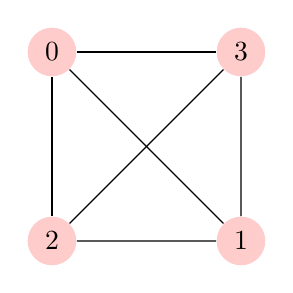
\begin{tikzpicture}
  [scale=.6,auto=left,every node/.style={circle,fill=red!20}]
  \node (n1) at (0,0) {0};
  \node (n2) at (4,-4)  {1};
  \node (n3) at (0,-4)  {2};
   \node (n4) at (4,0)  {3};

  \foreach \from/\to in { n1/n2,n1/n3,n1/n4,n2/n3,n2/n4,n3/n4}
    \draw (\from) -- (\to);

\end{tikzpicture}
\caption{A graph with four vertices and six edges}\label{1g1}
\end{center}
\end{figure}
\begin{newpage}
\end{newpage}

In our next example [Figure \ref{1g2}], we have five vertices representing five people, namely Bob, William, James, Chris, and Ajur. The edges in the graph represent friendship. Chris is friends with William, James, and Ajur. Bob is friends with William and James. These friendship relations are depicted as a graph with five vertices and five edges.
\begin{figure}
\begin{center}
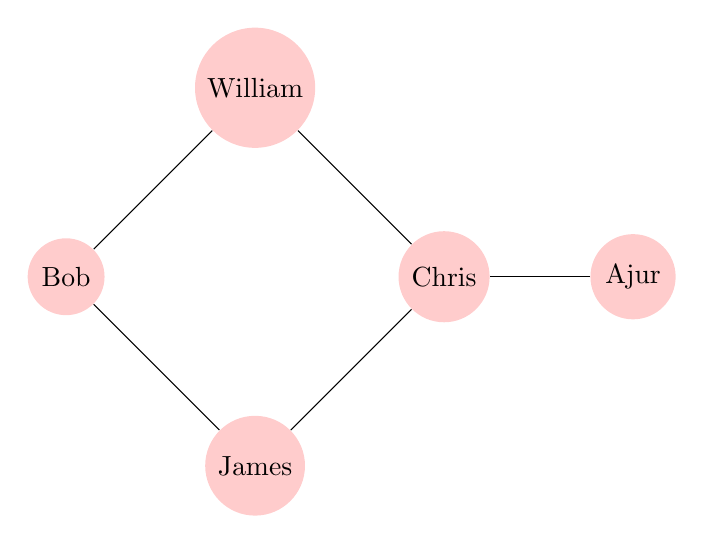
\begin{tikzpicture}
  [scale=.6,auto=left,every node/.style={circle,fill=red!20}]
  \node (n1) at (0,0) {Bob};
  \node (n2) at (4,4)  {William};
  \node (n3) at (4,-4)  {James};
   \node (n4) at (8,0)  {Chris};
    \node (n5) at (12,0) {Ajur};
  \foreach \from/\to in { n1/n2,n1/n3,n3/n4,n2/n4,n4/n5}
    \draw (\from) -- (\to);

\end{tikzpicture}
\caption{A friendship graph with five vertices and five edges}\label{1g2}
\end{center}
\end{figure}


\begin{newpage}
\end{newpage}
In our third example [Figure \ref{1g3}], we have seven Northeastern states in the United States, namely New York (NY), Connecticut (CT), Vermont (VT), Maine (ME), Massachusetts (MA), Rhode Island (RI), and New Hampshire (NH). The relationship represented in this graph is the sharing of a border with another state. Therefore, NY borders CT, VT, and MA. CT additionally borders RI and MA. VT additionally borders MA and NH. ME only borders NH. MA additionally borders RI and NH. These state-border relations are depicted as a graph with seven vertices and 10 edges.

\begin{figure}
\begin{center}
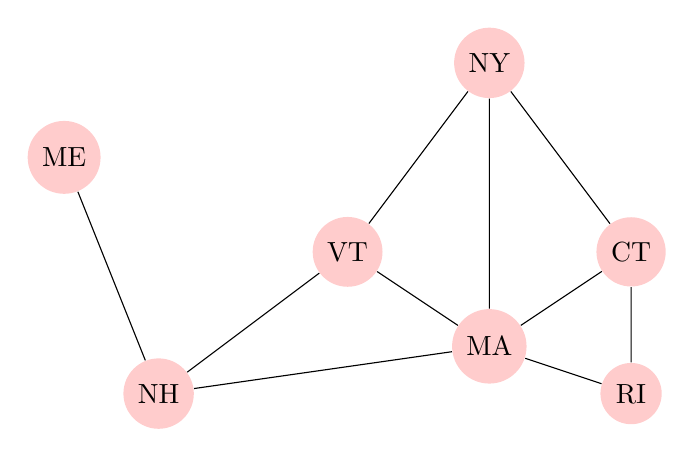
\begin{tikzpicture}
  [scale=.6,auto=left,every node/.style={circle,fill=red!20}]
  \node (n1) at (0,1) {ME};
  \node (n2) at (2,-4)  {NH};
  \node (n3) at (6,-1)  {VT};
   \node (n4) at (9, -3) {MA};
   \node (n5) at (9,3)  {NY};
    \node (n6) at (12,-1) {CT};
    \node (n7) at (12, -4) {RI};
  \foreach \from/\to in { n1/n2,n2/n3,n2/n4, n3/n4,n3/n5,n4/n5,n4/n6,n4/n7,n5/n6,n6/n7}
    \draw (\from) -- (\to);

\end{tikzpicture}
\caption{A graph representing seven Northeastern states in the United States, with seven vertices and 10 edges}\label{1g3}
\end{center}
\end{figure}

One other term to introduce here. If there is an edge between two vertices (e.g.,~between NY and VT in Figure~\ref{1g3}), we say that these two vertices are \textbf{adjacent}. More specifically, NY is adjacent to VT. And VT is adjacent to NY.

%\chapter{Introduction}
   

\chapter{A Trip to the Cemetery}
It was Halloween, a cold and dreary fall afternoon. Ajur was interested in visiting the famous cemetery in Royt as any teenager with an adventurous spirit would be wont to do. His pet dog Jura, a Labrador, was eager to follow. As Ajur examined the old headstones, he lost track of time, and it grew dark. He felt tired, so he and Jura sat under a tree and fell asleep.

Deep in sleep, they were awakened by a loud noise. The noise was from Rishnak, a ghost who lived in the cemetery. Rishnak had died many years ago; he used to teach mathematics and graph theory to talented high school students all throughout the area. When Rishnak spotted Ajur in the cemetery, he thought to himself, ``Here is an unusual teenager.'' Perhaps he could test whether this youngster was proficient in mathematics. And if he was indeed proficient, Rishnak could reward him with his magical powers. When Rishnak appeared in front of Ajur, Jura jumped up and started barking. Ajur sat up with a start.

Rishnak was afraid he would intimidate Ajur by being brusque. Jura's barking became louder and louder, so Rishnak started talking in a soft voice. He gently asked what grade Ajur was in. Ajur replied that he was in the 8th grade. Rishnak asked what subjects Ajur liked most in school, to which Ajur proudly said, ``mathematics.'' Rishnak smiled. He told the boy that he had been cursed to live as a ghost, and his curse could only be lifted if he could reward a youngster who could answer all of his questions.

Ajur was intrigued by Rishnak's plight. Standing up now, Ajur was excited for the possibility of rewards and the opportunity to help lift the curse on Rishnak, a poor ghost. Ajur also thought he would be able to tell his friends about his adventure.
\chapter{Degrees}
Rishnak asked Ajur whether he knew about graphs and trees in mathematics. Ajur jumped up and down and proclaimed that he knew all about graph theory. He continued that graphs are often used to  represent relations of a set of objects. He enthusiastically stated that the famous mathematician Euler was the father of graph theory. He was eager to show off his knowledge and described the famous  K\"{o}nigsberg bridge problem.  K\"{o}nigsberg (in modern day Russia) was on the banks of the Pregel river.  There were seven bridges across this river, connecting the two sides of the river and two islands. Ajur drew a graph of this on a piece of paper he was carrying.
\begin{figure}
\begin{center}
\includegraphics[width=0.6\textwidth]{konigsberg.JPG}
\caption{A Graph representing K\"{o}nigsberg Bridge. Vertices 1 and 3 are islands and 0 and 2 are the two riverbanks.}\label{kon}
\end{center}
\end{figure}

He continued that the problem was to start from the vertex labeled 0 and go through all bridges once and only once and return to the starting vertex 0. Ajur could not contain his enthusiasm and asked Rishnak how to do it. Rishnak gently reminded Ajur that he was the one asking questions and Ajur just had to respond with correct responses. Ajur nodded his head enthusiastically.

 Since this was the first time, Rishnak told Ajur that he was going to ask Ajur a series of questions and observe whether his curses could be lifted.
 
 Rishnak then asked Ajur, ``in a class of 33 students, what is the maximum and minimum number of friends a student can have?"\footnote{Being friend is a mutual relation, i.e. if A is a friend of B, then B is a friend of A. A student cannot be a friend to herself!}
 
 Ajur nonchalantly replied that the maximum number is 32 and the minimum number is 0.
 
 Rishnak then asked Ajur ``will there be a student in a class having 32 friends and a student having 0 friends?"
 
 Ajur smiled to himself that Rishnak seems like a clever ghost; Ajur replied, ``how is that possible --- if a student has 32 friends, so she is friends with everyone else, then everyone else has at least one friend. 
 So there cannot be a 
 student with 0 friends. Similarly if there is a student with 0 friends, there are only 32 students remaining and another student can have at most 31 friends."
 
 Rishnak was pleased to have found someone who seemed to have the ability to help him and the questioning continued. ``Can all the 33 students have a distinct number of friends?"
 
 Ajur responded immediately saying it is not possible because there are 33 distinct students, and the distinct number of friends the class can have is $\{0,1,2,\cdots,32\}$. There are 33 numbers in this, but alas it contains both students with 32 friends and with 0 friends. Ajur just had told Rishnak that it is not possible to have a student with 32 friends and another student with 0 friends.
 
 Rishnak asked Ajur, ``can there be just two students having the same number of friends, with the others all having distinct numbers of friends?" Rishnak further added that all of the students have at least one friend.
 
Ajur wanted to reason it out. He knew that the maximum number can only be 32, and the minimum has to be 1, so there are 32 distinct numbers. But there are 33 students. So by the pigeon hole principle --- if there are more pigeons than boxes, then one box contains at least two pigeons --- there have to be two students with the same number of friends.  He then reasoned about what the numbers could be. He matched 32 with 1: that is, the student having one friend has to be a friend of a student with 32 friends. Then he matched 2 with 31: the student with 2 friends has to be a friend of a student with 32 friends and a student with 31 friends. Continuing this argument, he matched 3 with 30, 4 with 29, $\cdots$, 15 with 18 and 16 with 17. We have an even number of students accounted for but an odd number of total students. That means there are two students having the same number of friends.

Rishnak posed the next question: He asked 5 students in a class of 6 students how many friends each of them have and they all gave distinct numbers greater than 0. How many friends does the student who was not asked have?

Ajur thought about this. If all the five students had given distinct numbers and they were greater than 0, they had to be $\{1,2,3,4,5\}$. Let the students be A(pu), B(art), C(arla), D(uma), E(rnie) having 5, 4, 3, 2 and 1 friends respectively. Let F(ermat) be the sixth student. A is friends with B, C, D, E and F. B is friends with C, D and F. B is already friends with A and E has only one friend, namely A. Now C is friends with F. C is already friends with A and B, and D and E have their friends quota counted already. 
Now it is easy to see that F(ermat) has exactly 3 friends, namely A, B and C.

Ajur drew the following graph as in Figure \ref{dg2}.

\begin{figure}
\begin{center}
\includegraphics[width=0.6\textwidth]{graphstory1-1.JPG}
\caption{A Graph with 6 students and 5 students having 5, 4, 3, 2 and 1 friends}\label{dg2}
\end{center}
\end{figure}

Rishnak was impressed, but wanted to test Ajur further. He asked whether there can an be odd number of students having odd number of friends. Ajur said that it is impossible as the sum of all numbers of friends across all students has to be even. He reasoned that if A is a friend of B, then this friendship is counted twice. Hence the sum of all friends of students is even. We know that the students having an even number of friends will contribute an even number of friendships. This in turn implies that the number of students having an odd number of friends has to be even.


Rishnak started asking, ``can you draw a graph of a class with 5 students respectively having 1, 2, 2, 2 and 1 friends?"

Ajur whipped up the graph drawn in Figure \ref{dg3}. 

\begin{figure}
\begin{center}
\includegraphics[width=0.6\textwidth]{graphstory1-2.JPG}
\caption{A Graph with 5 students having 2, 2, 2, 1 and 1 friends}\label{dg3}
\end{center}
\end{figure}

Rishnak asked whether one can draw another graph having the given friends list.\footnote{Hakimi has given a method of constructing a graph with a given degree sequence}

Ajur took no time to respond and drew another graph as in Figure \ref{dg4}.

\begin{figure}
\begin{center}
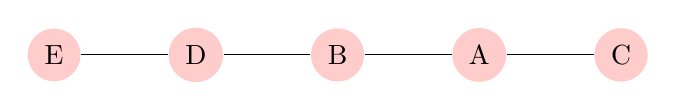
\begin{tikzpicture}
  [scale=.6,auto=left,every node/.style={circle,fill=red!20}]
  \node (n1) at (0,0) {E};
  \node (n2) at (3,0)  {D};
  \node (n3) at (6,0)  {B};
   \node (n4) at (9,0)  {A};
  \node (n5) at (12,0)  {C};
  \foreach \from/\to in { n1/n2,n2/n3,n3/n4,n4/n5}
    \draw (\from) -- (\to);

\end{tikzpicture} %\includegraphics[width=0.6\textwidth]{graphstory1-3.JPG}
\caption{Another Graph with 5 students having 2, 2, 2, 1 and 1 friends}\label{dg4}
\end{center}
\end{figure}

Jura was waking up and wanted to play with Ajur. Rishnak was happy to see the answers that Ajur gave. He saw a ray of hope that his curse could be lifted. 

\textbf{Question for the first day:}  Provide a degree sequence that is the degree sequence of only one graph? (You can ignore the labels on vertices.)

\textbf{Answer:} Ajur said that the degree sequence of all 0's have only one graphical realization!

\textbf{Followup Question:}Rishnak said he agreed to Ajur's answer. Is there a degree sequence with only one graph realizing it and having one or mode edges?

\textbf{Answer:} Ajur responded for a sequence of even length, a degree sequence, of $1,1,\cdots, 1$ will be realized by a unique graph.

He showed an example with $1,1,1,1,1,1,1,1$ in the following Figure \ref{daya1}

\begin{figure}
\begin{center}
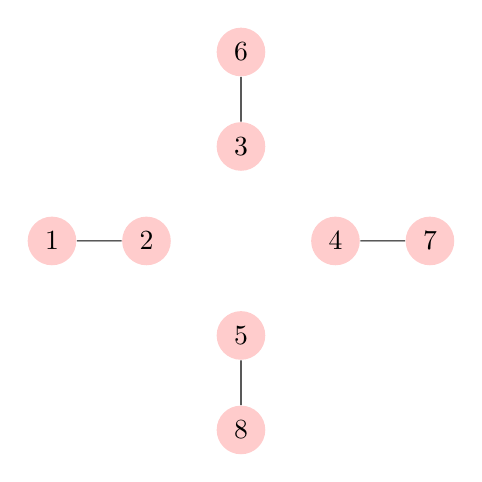
\begin{tikzpicture}
  [scale=.6,auto=left,every node/.style={circle,fill=red!20}]
  \node (n1) at (1,7) {1};
  \node (n2) at (3,7)  {2};
  \node (n4) at (7,7) {4};
  \node (n7) at (9,7)  {7};
  \node (n6) at (5,11)  {6};
   \node (n3) at (5,9) {3};
   \node (n5) at (5,5) {5};
   \node (n8)  at (5,3) {8};
  \foreach \from/\to in {n1/n2,n3/n6,n4/n7,n5/n8}
   \draw (\from) -- (\to);

\end{tikzpicture}
\caption{ Unique Graph with degree sequence 1,1,1,1,1,1,1,1 }\label{daya1}
\end{center}
\end{figure}

Rishnak told Ajur to come back the next night, and he disappeared in a cold mist.
%\chapter{Puzzle 2}
\chapter{Rooted Trees and Trees}

Rishnak found Ajur and his dog Jura walking along a row of graves. Ajur was reading the inscriptions on the tombstones. Each headstone had the names of the family (parents, wife, husband) and the dates of birth and of death. Ajur did not know so many relatives could be buried in such a small area. He then thought of how different cultures honor their departed ones. \footnote{He remembered seeing the movie Coco in 2017 about how people in Mexico remember their departed ones. He had also heard how Hindus in India go to the city of Banaras/Varanasi to perform rituals to thank and honor their deceased forefathers.} 
Ajur remembered the definition of a tree and a rooted tree. He was talking to Jura, saying that a rooted tree in graph theory/mathematics looks like a normal tree with a distinguished vertex. A rooted tree in real life has a root at the bottom whereas a rooted tree in graph theory is drawn with a root at the top. Both of them convey the same information.

``Here are two drawings of the same information." Ajur further explained that each vertex in a rooted tree has just one parent vertex (except the root vertex, which has no parent). A rooted tree can also be thought of as a graph with a collection of vertices and edges. There are some restrictions. But that will become clearer, as the story proceeds.


\begin{figure}
\begin{center}
\includegraphics[width=\textwidth]{tree1.JPG}
\caption{A Tree drawn with a root at the bottom}\label{rg1}
\end{center}
\end{figure}

\begin{figure}
\begin{center}
\includegraphics[width=\textwidth]{tree2.JPG}
\caption{Same Tree drawn with a root at the top}\label{rg2}
\end{center}
\end{figure}

Rishnak caught up with Ajur and Jura as he had been following them quietly. Rishnak asked Ajur: ``How many edges does a rooted tree with 7 vertices have?" Ajur reasoned that since each vertex other than the root has exactly one parent vertex and there are no other edges, then number of edges will be 6. Rishnak then asked how many edges a rooted tree with 1000 vertices has. Ajur shot back with his answer 999. Impressed, but not unduly, Rishnak asked how many edges there are in a rooted tree with $n$ vertices. Nonchalantly, Ajur replied it is $n-1$ by the same argument (each of the $n-1$ vertices have just one edge connected to its parent).  

For each vertex other than a root vertex, there is a parent vertex and zero or more child vertices.  The descendants of a vertex are all its children, grandchildren, great grandchildren vertices, etc. Analogously, for each vertex the ancestors of that vertex are its parent, grandparent, great grandparent vertices, etc. 
A vertex with no child vertices is known as a leaf vertex. Rishnak asked Ajur ``What is the largest number of leaf vertices a tree with 6 vertices can have?" Ajur immediately responded that the number is 5, and he drew a rooted tree as in Figure \ref{t1}.

\begin{figure}
\begin{center}
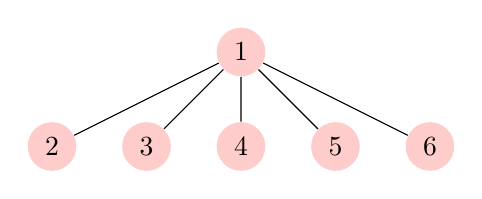
\begin{tikzpicture}
  [scale=.6,auto=left,every node/.style={circle,fill=red!20}]
  \node (n6) at (5,5) {1};
  \node (n4) at (1,3)  {2};
  \node (n5) at (3,3)  {3};
  \node (n1) at (5,3) {4};
  \node (n2) at (7,3)  {5};
  \node (n3) at (9,3)  {6};

  \foreach \from/\to in {n6/n1,n6/n2,n6/n3,n6/n4,n6/n5}
    \draw (\from) -- (\to);

\end{tikzpicture}
\caption{A Tree with 6 vertices and 5 leaf vertices. The vertex labeled 1 is the root vertex}\label{t1}
\end{center}
\end{figure}

Rishnak asked, ``What is the smallest number of leaf vertices a tree with 6 vertices can have?" Ajur knew this answer too. So he drew a rooted tree as in Figure~\ref{t2}.

\begin{figure}
\begin{center}
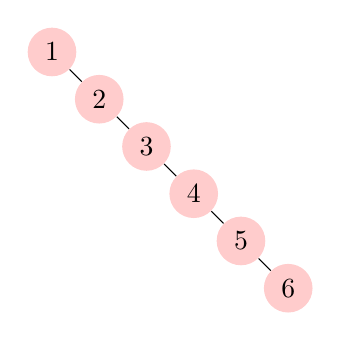
\begin{tikzpicture}
  [scale=.6,auto=left,every node/.style={circle,fill=red!20}]
  \node (n6) at (3,7) {1};
  \node (n4) at (4,6)  {2};
  \node (n5) at (5,5)  {3};
  \node (n1) at (6,4) {4};
  \node (n2) at (7,3)  {5};
  \node (n3) at (8,2)  {6};

  \foreach \from/\to in {n6/n4,n4/n5,n5/n1,n1/n2,n2/n3}
    \draw (\from) -- (\to);

\end{tikzpicture}

\caption{A Tree with 6 vertices and one leaf vertex labeled 6. The vertex labeled 1 is the root vertex.}\label{t2}
\end{center}
\end{figure}

Rishnak said, ``We get a lot of lightning and thunderstorms here, especially during summer months. Lightning affects tall objects, especially objects that conduct electricity in an open area.\footnote{Benjamin Franklin had demonstrated the electrical nature of lightning.} Lightning conductors are usually at the top of the buildings and have less resistance than the building and hence lightning passes through the conductor." Rishnak drew a rooted tree with 3 vertices as shown in Figure~\ref{t3}.

\begin{figure}
\begin{center}

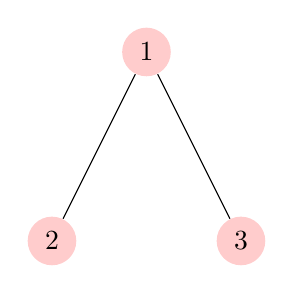
\begin{tikzpicture}
  [scale=.6,auto=left,every node/.style={circle,fill=red!20}]
  \node (n1) at (3,7) {1};
  \node (n2) at (1,3)  {2};
  \node (n3) at (5,3)  {3};


  \foreach \from/\to in {n1/n2,n1/n3}
    \draw (\from) -- (\to);

\end{tikzpicture}

\caption{A resistance  Tree with 3 vertices and two leaf vertices at the ground. }\label{t3}
\end{center}
\end{figure}


Rishnak said that the each edge has a resistance of 1 ohm, and vertices labeled 2 and 3 are grounded. What is the effective resistance of the resistance tree in Figure~\ref{t3}? Ajur remembered his physics and he realized two resistances are in parallel. So he immediately replied that the effective resistance is $\frac{1}{2}$ ohms. (Intuitively, there are two paths the current can take and hence the resistance splits evenly between the two paths).

Rishnak asked the same question, effective resistance, for the following rooted tree shown in Figure \ref{t4}.
\begin{figure}
\begin{center}

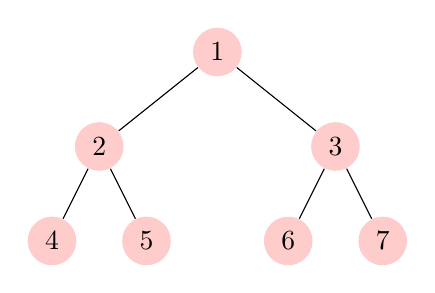
\begin{tikzpicture}
  [scale=.6,auto=left,every node/.style={circle,fill=red!20}]
  \node (n1) at (5.5,7) {1};
  \node (n2) at (3,5)  {2};
  \node (n3) at (8,5)  {3};
  \node (n4) at (2,3) {4};
  \node (n5) at (4,3)  {5};
  \node (n6) at (7,3)  {6};
  \node (n7) at (9,3)  {7};

  \foreach \from/\to in {n1/n2,n1/n3,n2/n4,n2/n5,n3/n6,n3/n7}
    \draw (\from) -- (\to);

\end{tikzpicture}

\caption{A resistance  Tree with 7 vertices and four leaf vertices at the ground. }\label{t4}
\end{center}
\end{figure}

Ajur said that he had computed the effective resistances for trees rooted at vertex labeled 2 and 3 to be $\frac{1}{2}$. There are two parallel paths with equal resistance of $1+\frac{1}{2}$ (There is a series connection from root vertex 1 and vertices labeled 2 and 3 respectively). Hence the effective resistance is $\frac{3}{4}$ ohms. Ajur further said that there is a pattern here. For the resistance tree with 15 vertices (adding one more level or increasing the height), the effective resistance will be $\frac{7}{8}$. Rishnak then asked what happens if the tree is of infinite height! (A really tall lightning conductor.) Ajur was perplexed - But, then, he reasoned that this could be formulated as a recurrence relation. Let R be the effective resistance of this infinite tree. The root has two children, each of which will have a resistance of R ohms. The root vertex is connected to the child vertex with a resistance of 1 ohm. Hence he wrote an equation $$R= \frac{R+1}{2}$$ Simplifying this, he got the resistance of 1 ohm. A tree of infinite height with its very low resistance is like a really tall and effective lightning conductor.\footnote{Because of a large number of joints, this solution may not be a practical one!} Rishnak responded that there is another way of getting the same result. From an earlier example, you can generalize the resistance to be $\frac{2^h-1}{2^h}$ , $h$ being height (longest among path lengths from the root vertex to all leaf vertices) of the rooted tree. This can be further simplified to be $1-\frac{1}{2^h}$. As $h$ goes to infinity the term $\frac{1}{2^h}$ goes to 0 and hence the resistance is 1. Ajur learned an important lesson that there are multiple ways of getting a solution and each one may provide a new insight. Ajur asked Rishnak: ``Can you construct an infinite height tree (with edge resistances being 1 ohm) so that the effective resistance is $\frac{1}{2}$, $\frac{1}{3}$, $\frac{1}{4}$ or more generally any fraction $\leq$~1?" Rishnak replied to Ajur that he was the one who could ask questions and not Ajur.\footnote{Of course, Rishnak knew the answer and suggests others to think of every vertex having more than 2 child vertices!}

A tree is like a rooted tree but with no root vertex. A tree can be drawn in any manner. The degree of a vertex is the number of edges incident on that vertex. The leaf (pendant) vertex has a degree of 1. So in Figure~\ref{t2} both vertices labeled 1 and 6 are leaf/pendant vertices and all other vertices have degree 2. 

Rishnak told Ajur that one important property of a tree is that there are no cycles in it. Ajur could easily understand it from a genealogy perspective - a person cannot be an ancestor as well as a descendant of himself/herself.  Ajur added that there is only one path between any two vertices in a tree (Of course, Ajur assumed that the edges are undirected - which Rishnak knew). Rishnak asked ``how did you infer that there is a unique path between two vertices in a tree?" Ajur promptly replied that if there are two paths between any two vertices, there will be a cycle (which cannot exist in a tree). Since there is a unique path between two vertices, one can compute the distance between two vertices as the number of edges in that path. Ajur provided clarifications with examples.  As an example in Figure~\ref{t1}, the distance between the vertex labeled 1 and any other vertex is 1. The distance between the vertex labeled 2 and the vertex labeled 6 is 2. In Figure~\ref{t2}, the distance between the vertex labeled 1 and the vertex labeled 6 is 5 and the distance between the vertex labeled 2 and the vertex labeled 4 is 2.
%(Dad: you could also add the fact that every finite tree has a center of mass! it's in this vein, and not especially well known (Boris hadn't realized it!))

\textbf{Question for the second day:} Construct an infinite tree with resistance of $\frac{3}{5}$.

\textbf{Answer:} Ajur said a way to think about this is to consider an infinite tree in which vertex has 6 children and each edge is of resistance 3 ohms (We can add a series of three 1 ohm edges to get 3 ohms).
With this we will get a recurrence equation $R=\frac{R+3}{6}$ - that is, each child vertex will have a resistance of R ohms (by symmetry as they look like the original tree). Simplifying this, we will get a $\frac{5R}{6}=\frac{3}{6}$ which simplifies to a resistance, R, of $\frac{3}{5}$ ohms.

Rishnak was very pleased. They called it a day.
\chapter{Subgraphs}
Rishnak wandered the cemetery, looking for Ajur. As he searched, he saw a headstone with the name Schossow. Rishnak recognized the name from the ``Instant Insanity'' puzzle{\footnote{This is also known as Katzenjammer, (Great) Tantalizer, Face-4, Cube-4, Bognar Balls, Taktikolor, Frantic, Diabolical, Damblocks, and Symington's Puzzle. A patent was awarded to Schossow in 1990.}}, and just as Rishnak was thinking it would be an interesting topic to discuss with Ajur, Jura the dog, eager to explore, nudged Ajur awake from a nap.

Before long, Ajur and Jura were strolling along the path when Rishnak startled Ajur (as ghosts tend to do).

Rishnak asked Ajur what he knew about subgraphs. Ajur said that he was familiar with subsets. ``And since a graph has both a vertex set and an edge set, I think I can deduce what a subgraph is. Given some graph~$G=(V,E)$ with vertex set~$V$ and edge set~$E$, then take any subset~$X$ of~$V$ and consider all edges in~$E$ for which both end vertices are in~$X$.''

Ajur picked up a stick and drew a graph in the dirt [Figure~\ref{3g}].

He said, ``From this first graph, I could define a separate vertex subset~$V'=\{1,2,3,5\}$ to form another graph, say~$G'=(V',E')$, which is a subgraph of the first.''

He drew a second graph [Figure~\ref{3g1}].

\begin{figure}
\begin{center}
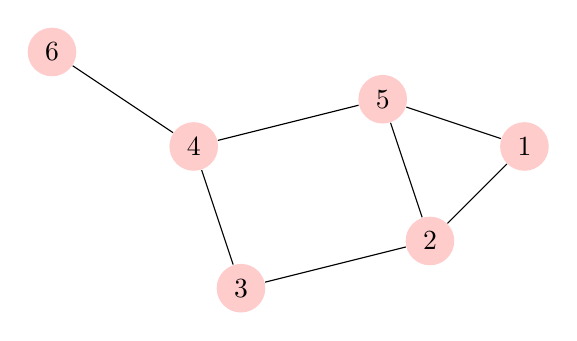
\begin{tikzpicture}
  [scale=.6,auto=left,every node/.style={circle,fill=red!20}]
  \node (n6) at (1,10) {6};
  \node (n4) at (4,8)  {4};
  \node (n5) at (8,9)  {5};
  \node (n1) at (11,8) {1};
  \node (n2) at (9,6)  {2};
  \node (n3) at (5,5)  {3};

  \foreach \from/\to in {n6/n4,n4/n5,n5/n1,n1/n2,n2/n5,n2/n3,n3/n4}
    \draw (\from) -- (\to);

\end{tikzpicture}
\caption{Example graph with six vertices and seven edges}\label{3g}
\end{center}
\end{figure}


\begin{figure}
\begin{center}
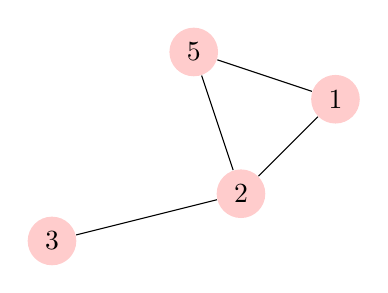
\begin{tikzpicture}
  [scale=.6,auto=left,every node/.style={circle,fill=red!20}]
  %\node (n6) at (1,10) {6};
  %\node (n4) at (4,8)  {4};
  \node (n5) at (8,9)  {5};
  \node (n1) at (11,8) {1};
  \node (n2) at (9,6)  {2};
  \node (n3) at (5,5)  {3};

  \foreach \from/\to in {n5/n1,n1/n2,n2/n5,n2/n3}
    \draw (\from) -- (\to);
\end{tikzpicture}
\caption{Induced subgraph of the graph shown in Figure~\ref{3g}, with vertices in set $V'=\{1,2,3,5\}$ and all edges between these vertices present from the original graph}\label{3g1}
\end{center}
\end{figure}

Rishnak laughed and said that the subgraph Ajur drew was called an \textit{induced subgraph}. He said, ``It is called that because all of the edges are included in the vertex subset. You do have the flexibility of choosing only a subset of these edges, but there is one condition: for each edge in the chosen subset of edges, the end vertices must be in the chosen vertex subset. Let me show you.''

Rishnak drew a graph in the air in a dazzling light display [Figure~\ref{3g2}]. ``Here is a subgraph of your original graph. And note that a subgraph with no vertices and no edges is also an induced subgraph (and subgraph) of any graph.''

\begin{figure}
\begin{center}
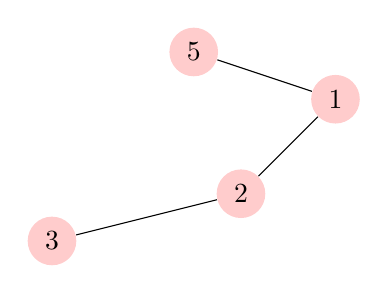
\begin{tikzpicture}
  [scale=.6,auto=left,every node/.style={circle,fill=red!20}]
  %\node (n6) at (1,10) {6};
  %\node (n4) at (4,8)  {4};
  \node (n5) at (8,9)  {5};
  \node (n1) at (11,8) {1};
  \node (n2) at (9,6)  {2};
  \node (n3) at (5,5)  {3};

  \foreach \from/\to in {n5/n1,n1/n2,n2/n3}
    \draw (\from) -- (\to);

\end{tikzpicture}
\caption{A subgraph of Figure~\ref{3g}}\label{3g2}
\end{center}
\end{figure}


%Rishnak said that in a graph having $n$ vertices where the vertices are labeled (have a number/name associated with them), then there are at least $2^n$ subgraphs and exactly $2^n$ induced subgraphs.  There are ${n \choose i}$ ways of choosing $i$ vertices from a given set of $n$ vertices. Once the vertices are chosen, the edges are fixed for an induced subgraph. Since $i$ can vary from 0 to $n$, we get $2^n$ induced subgraphs. Since every induced subgraph is a subgraph (and not every subgraph is not an induced subgraph), we have at least $2^n$ subgraphs.  

Ajur nodded his head and yawned.
Rishnak scowled and said, ``Time to learn something new, Ajur, then see if you can still answer my questions.''

Ajur straightened as Rishnak continued. ``A walk from a vertex~$i$ to a vertex~$j$ is an alternating sequence of vertices and edges. Every edge in that walk is incident between vertices preceding and succeeding that edge. For example, in that graph that you drew''---he pointed down to the dirt [Figure~\ref{3g}]---``a walk from vertex~6 to vertex~1 could be $6-(6,4)-4-(4,3)-3-(3,2)-2-(2,1)-1$. The edges are represented as a vertex pair. And if those edges have names as labels, we could use that label instead. Another walk from vertex~6 to vertex~1 could be $6-(6,4)-4-(4,5)-5-(5,1)-1$.''

Ajur listened intently, then asked, ``Can a walk use the same edge more than once?''

Rishnak said, ``No. The only other condition that a walk has (besides an edge being incident on a preceding and a succeeding vertex) is that all edges must be distinct. The vertices in a walk can be repeated, though. Have a look at this graph.'' In a flash of light, Rishnak drew another graph [Figure~\ref{3g3}]. ``A walk from vertex~1 to vertex~8 could be $1-(1,2)-2-(2,4)-4-(4,6)-6-(6,8)-8-(8,2)-2-(2,3)-3-(3,4)-4-(4,5)-5-(5,6)-6-(6,7)-7-(7,8)-8$.''

Ajur tried to pay attention but was naturally getting bored. He interjected, ``In your walk, you have visited all the edges in the graph, much like the K\"{o}nigsberg Bridge Problem.''\footnote{As mentioned earlier in Chapter 3 [Figure~\ref{kon}].}

\begin{figure}
\begin{center}
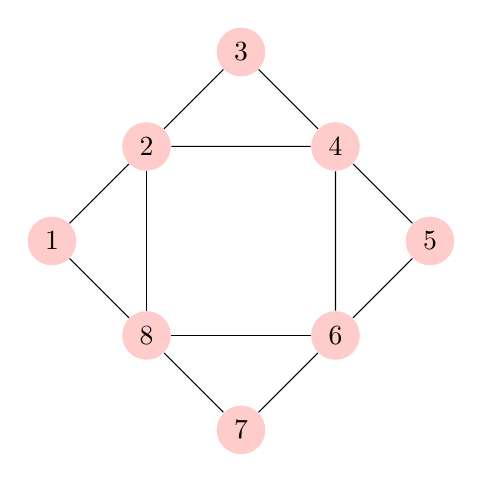
\begin{tikzpicture}
  [scale=.6,auto=left,every node/.style={circle,fill=red!20}]
  \node (n1) at (1,7) {1};
  \node (n2) at (3,9)  {2};
  \node (n3) at (5,11)  {3};
  \node (n4) at (7,9) {4};
  \node (n5) at (9,7)  {5};
  \node (n6) at (7,5)  {6};
  \node (n7) at (5,3)  {7};
  \node (n8) at (3,5)  {8};

  \foreach \from/\to in {n1/n2,n1/n8,n2/n3,n2/n4,n2/n8,n3/n4,n4/n5,n4/n6,n5/n6,n6/n7,n6/n8,n7/n8}
    \draw (\from) -- (\to);

\end{tikzpicture}
\caption{Example graph with eight vertices and 12 edges}\label{3g3}
\end{center}
\end{figure}

Rishnak smiled and nodded. ``And if the starting and ending vertices in a walk are the same, it is known as a closed walk. If all of the edges in a closed walk are distinct, then it is known as a cycle.''

Ajur remembered the idea of a cycle from yesterday's discussion of trees.

Rishnak asked Ajur to list two cycles from the graph that sparkled in front of him [Figure~\ref{3g3}].

Ajur had no trouble at all in listing two cycles as $1-(1,2)-2-(2,8)-8-(8,1)-1$ and $2-(2,4)-4-(4,6)-6-(6,8)-8-(8,2)-2$. Rishnak taught Ajur that often the edges are omitted when describing a walk, so the cycles could be written simply as $(1,2,8,1)$ and $(2,4,6,8,2)$. And even simpler, we can state that a walk is a cycle and omit the repetitive last vertex, so we have cycles $(1,2,8)$ and $(2,4,6,8)$.

Rishnak beamed as he went on.  ``Of course a cycle and a walk are examples of subgraphs with some added conditions. These added conditions make the study of subgraphs very interesting. If in a cycle, all the vertices of the original graph are present, then that cycle is known as a Hamiltonian Cycle. For example, in this graph''---he again referred to the graph that shone in front of him [Figure~\ref{3g3}]---``the cycle $(1,2,3,4,5,6,7,8,1)$ is a Hamiltonian Cycle of this other graph''---he whisked his hands through the air to produce another graph [Figure~\ref{3g4}]---``And if all the edges in a walk are distinct then it is known as a path.''

\begin{figure}
\begin{center}
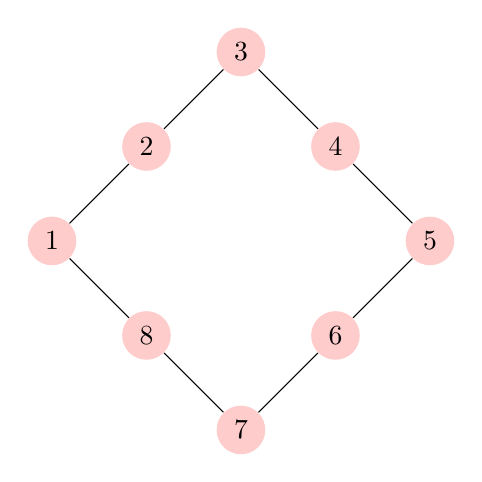
\begin{tikzpicture}
  [scale=.6,auto=left,every node/.style={circle,fill=red!20}]
  \node (n1) at (1,7) {1};
  \node (n2) at (3,9)  {2};
  \node (n3) at (5,11)  {3};
  \node (n4) at (7,9) {4};
  \node (n5) at (9,7)  {5};
  \node (n6) at (7,5)  {6};
  \node (n7) at (5,3)  {7};
  \node (n8) at (3,5)  {8};

  \foreach \from/\to in {n1/n2,n1/n8,n2/n3,n3/n4,n4/n5,n5/n6,n6/n7,n7/n8}
    \draw (\from) -- (\to);

\end{tikzpicture}
\caption{A subgraph of Figure~\ref{3g3}, which forms a Hamiltonian Cycle}\label{3g4}
\end{center}
\end{figure}


Ajur tried to keep up.  ``Okay, so in that first graph''---he pointed to the graph [Figure~\ref{3g3}]---``an example path is $1-(1,2)-2-(2,3)-3$ or simply $(1,2,3)$. Let me draw this path.'' He drew the path in the dirt [Figure~\ref{3g5}].

\begin{figure}
\begin{center}
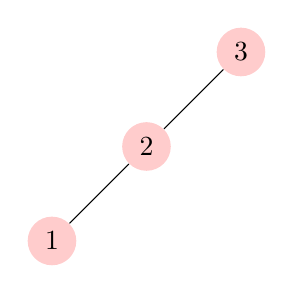
\begin{tikzpicture}
  [scale=.6,auto=left,every node/.style={circle,fill=red!20}]
  \node (n1) at (1,7) {1};
  \node (n2) at (3,9)  {2};
  \node (n3) at (5,11)  {3};

  \foreach \from/\to in {n1/n2,n2/n3}
    \draw (\from) -- (\to);

\end{tikzpicture}
\caption{A subgraph of Figure~\ref{3g3}, which forms a tree}\label{3g5}
\end{center}
\end{figure}

Rishnak nodded, then continued, ``If there is a path between every pair of vertices in a subgraph, then the subgraph is said to be connected. If a subgraph contains no cycles and is connected, the subgraph is a tree. And if such a tree contains all of the vertices then it is known as a spanning tree since it spans all vertices. Watch closely, here's a spanning tree.''

Rishnak transformed the original graph [Figure~\ref{3g3}] into a new one with fewer edges [Figure~\ref{3g6}].

\begin{figure}
\begin{center}
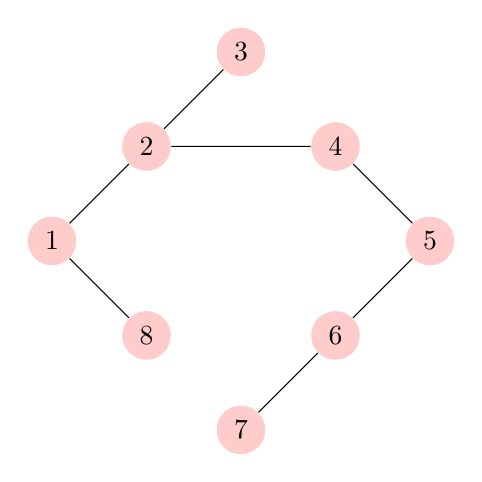
\begin{tikzpicture}
  [scale=.6,auto=left,every node/.style={circle,fill=red!20}]
  \node (n1) at (1,7) {1};
  \node (n2) at (3,9)  {2};
  \node (n3) at (5,11)  {3};
  \node (n4) at (7,9) {4};
  \node (n5) at (9,7)  {5};
  \node (n6) at (7,5)  {6};
  \node (n7) at (5,3)  {7};
  \node (n8) at (3,5)  {8};

  \foreach \from/\to in {n1/n2,n1/n8,n2/n3,n2/n4,n4/n5,n5/n6,n6/n7}
    \draw (\from) -- (\to);

\end{tikzpicture}
\caption{A subgraph of Figure~\ref{3g3}, which forms a spanning tree}\label{3g6}
\end{center}
\end{figure}

Rishnak continued, ``A subgraph in which the degree of every vertex is~1 is said to be a matching. An example of a subgraph that is a matching for this original graph''---he again showed the original graph [Figure~\ref{3g3}]---``is this other graph that contains pairs of vertices.'' Rishnak moved his hands and the graph reduced to one with only three edges [Figure~\ref{3g7}].

``If the subgraph contains all vertices and the degree of every vertex is~1, then it is called a perfect matching. Here's an example of a subgraph that is a perfect matching.'' A new graph appeared, this time with all of the original vertices but only four edges [Figure~\ref{3g8}].

Rishnak asked Ajur how many perfect matchings there were in the original graph [Figure~\ref{3g3}].

Ajur thought for a bit, his brain catching up with everything Rishnak was showing him. He saw that vertices~1, 3, 5, and~7 have degree~2. Therefore, one of those incident on~1, 3, 5, and~7 would have to be selected. ``There are exactly two perfect matchings.''

\begin{figure}
\begin{center}
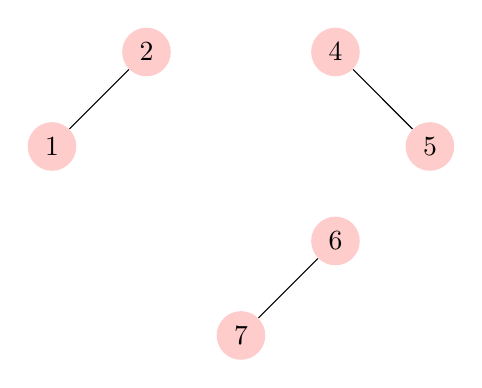
\begin{tikzpicture}
  [scale=.6,auto=left,every node/.style={circle,fill=red!20}]
  \node (n1) at (1,7) {1};
  \node (n2) at (3,9)  {2};
  %\node (n3) at (5,11)  {3};
  \node (n4) at (7,9) {4};
  \node (n5) at (9,7)  {5};
  \node (n6) at (7,5)  {6};
  \node (n7) at (5,3)  {7};
  %\node (n8) at (3,5)  {8};

  \foreach \from/\to in {n1/n2,n4/n5,n6/n7}
    \draw (\from) -- (\to);

\end{tikzpicture}
\caption{A subgraph of Figure~\ref{3g3}, which forms a matching}\label{3g7}
\end{center}
\end{figure}

\begin{figure}
\begin{center}
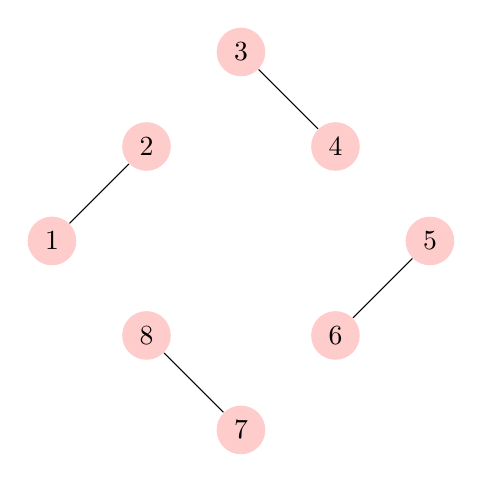
\begin{tikzpicture}
  [scale=.6,auto=left,every node/.style={circle,fill=red!20}]
  \node (n1) at (1,7) {1};
  \node (n2) at (3,9)  {2};
  \node (n3) at (5,11)  {3};
  \node (n4) at (7,9) {4};
  \node (n5) at (9,7)  {5};
  \node (n6) at (7,5)  {6};
  \node (n7) at (5,3)  {7};
  \node (n8) at (3,5)  {8};

  \foreach \from/\to in {n1/n2,n3/n4,n5/n6,n7/n8}
    \draw (\from) -- (\to);

\end{tikzpicture}
\caption{A subgraph of Figure~\ref{3g3}, which forms a perfect matching}\label{3g8}
\end{center}
\end{figure}

Rishnak had more to teach Ajur.  He said, ``A graph is connected if there is a path between every pair of vertices in that graph. Otherwise the graph is disconnected. Watch closely as here are two graphs, the first being a connected graph [Figure~\ref{3g9}], the second a graph that is not connected [Figure~\ref{3g10}].''

\begin{figure}
\begin{center}
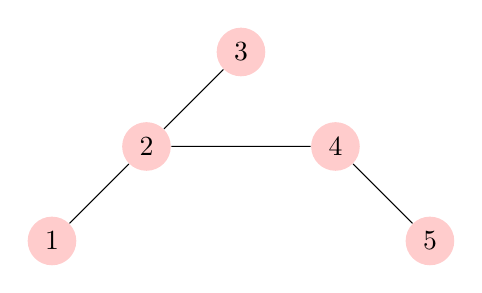
\begin{tikzpicture}
  [scale=.6,auto=left,every node/.style={circle,fill=red!20}]
  \node (n1) at (1,7) {1};
  \node (n2) at (3,9)  {2};
  \node (n3) at (5,11)  {3};
  \node (n4) at (7,9) {4};
  \node (n5) at (9,7)  {5};
\foreach \from/\to in {n1/n2,n2/n3,n2/n4,n4/n5}
    \draw (\from) -- (\to);

\end{tikzpicture}
\caption{A connected graph}\label{3g9}
\end{center}
\end{figure}

\begin{figure}
\begin{center}
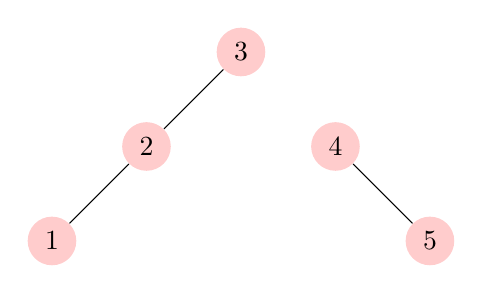
\begin{tikzpicture}
  [scale=.6,auto=left,every node/.style={circle,fill=red!20}]
  \node (n1) at (1,7) {1};
  \node (n2) at (3,9)  {2};
  \node (n3) at (5,11)  {3};
  \node (n4) at (7,9) {4};
  \node (n5) at (9,7)  {5};
\foreach \from/\to in {n1/n2,n2/n3,n4/n5}
    \draw (\from) -- (\to);

\end{tikzpicture}
\caption{A graph that is not connected}\label{3g10}
\end{center}
\end{figure}
\vspace{3in}

\subsection*{Question for the third day}
Rishnak said, ``At last we come to the question for the third day.  Can you list the cycles in this graph? And state the length of each cycle?'' He splayed his hands and a new graph appeared in front of him [Figure~\ref{day3g1}]

\begin{figure}
\begin{center}
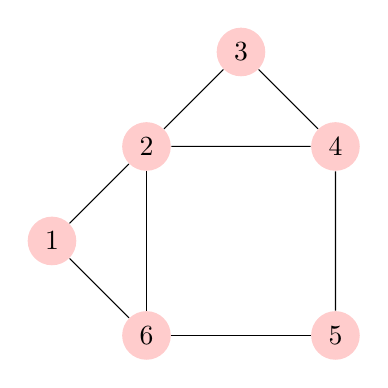
\begin{tikzpicture}
  [scale=.6,auto=left,every node/.style={circle,fill=red!20}]
  \node (n1) at (1,7) {1};
  \node (n2) at (3,9)  {2};
  \node (n3) at (5,11)  {3};
  \node (n4) at (7,9) {4};
  \node (n5) at (7,5)  {5};
  \node (n6) at (3,5)  {6};

  \foreach \from/\to in {n1/n2,n1/n6,n2/n3,n2/n4,n2/n6,n3/n4,n4/n5,n5/n6}
    \draw (\from) -- (\to);

\end{tikzpicture}
\caption{Can you list the cycles in this graph?}\label{day3g1}
\end{center}
\end{figure}

\textit{Before you turn the page, try to come up with an answer of your own!}

\newpage
\subsection*{Answer for the third day}
Ajur scratched his head and studied the graph that Rishnak showed him.  At length, he said, ``I think I see six cycles in the graph.'' He proceeded to list them.
\begin{itemize}
    \item Two cycles of length 3: $(1,2,6), (2,3,4)$
    \item One cycle of length 4: $(2,4,5,6)$
    \item Two cycles of length 5: $(2,3,4,5,6), (1,2,4,5,6)$
    \item One cycle of length 6: $(1,2,3,4,5,6)$
\end{itemize}

Rishnak was again pleased as this was the correct answer. He smiled and noticed that Ajur was getting restless, and so was Jura, so they called it a night.
\chapter{Euler Paths/Cycles}

Ajur was tired after listening to so many definitions and examples. He complained to Jura that the recent conversations with Rishnak were too similar to a math class and that he preferred to solve fun problems based on math concepts instead.  Rishnak overheard this conversation. Rishnak had to agree that that the previous day's exchange was dry. His small friends were right -- he was making the beautiful subject of graph theory dull and monotonous.

So, for the next session, Rishank chose a more interesting problem - the existence of an Eulerian walk. 

Recall that a connected graph is a graph where there is a path between every two vertices. Then an \emph{Eulerian walk} in a connected graph is a walk that includes every edge exactly once. If the starting vertex and the ending vertex are the same then the walk is called a \emph{closed Eulerian walk}. The problem is named in honor of was Leonhard Euler, who was the first person to state it.

The question of whether or not a given connected graph has an Eulerian walk or a closed Eulerian walk are among the oldest problems in graph theory. Rishnak caught up with Ajur and Jura walking along a desolate road in a far corner of the cemetery. Rishnak asked Ajur the following question: in the graph of Figure \ref{4g1}, is there is a walk starting from vertex 2 and ending at vertex 4 passing all of the edges \textbf{exactly once}? (This is what is known as an Eulerian walk. This is exactly like can you trace all the edges once and only once without lifting your pen.) Ajur saw there is a cycle (2,3,4,1,2). After this cycle, there is just one edge (2,4) left. Hence Ajur constructed an Eulerian walk by combining the two as (2,(2,3),3,(3,4),4,(4,1),1,(1,2),2,(2,4),4) or written simply as (2,3,4,1,2,4) by omitting the edges. Ajur illustrated this Figure \ref{4g15} Ajur further added that there is no closed Eulerian walk as that would necessarily imply that every vertex had even degree!


\begin{figure}
\begin{center}
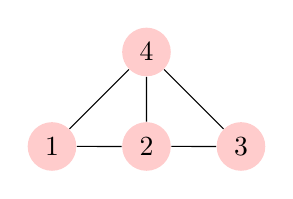
\begin{tikzpicture}
  [scale=.6,auto=left,every node/.style={circle,fill=red!20}]
  \node (n1) at (1,7) {1};
  \node (n2) at (3,7)  {2};
  \node (n3) at (5,7)  {3};
  \node (n4) at (3,9)  {4};

  \foreach \from/\to in {n1/n2,n2/n3,n2/n4,n1/n4,n3/n4}
    \draw (\from) -- (\to);

\end{tikzpicture}
\caption{ Example Graph with 4 vertices and 5 edges}\label{4g1}
\end{center}
\end{figure}

\begin{figure}
\begin{center}
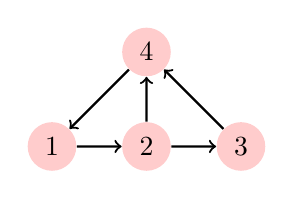
\begin{tikzpicture}
  [scale=.6,auto=left,every node/.style={circle,fill=red!20}]
  \node (n1) at (1,7) {1};
  \node (n2) at (3,7)  {2};
  \node (n3) at (5,7)  {3};
  \node (n4) at (3,9)  {4};

\path [->,draw,thick]
(n2) edge  (n3)
(n3) edge   (n4)
(n4) edge   (n1)
(n1) edge   (n2)
(n2) edge  (n4)
;
\end{tikzpicture}
\caption{ Eulerian Path from vertex 2 to vertex 4 2-3-4-1-2-4 of Figure \ref{4g1}}\label{4g15}
\end{center}
\end{figure}
\vspace{2cm}
Rishnak decided to make the problem more challenging and asked Ajur the following: in the graph of Figure \ref{4g2}, is there a walk from vertex 1 and end at vertex 9 and that traverses every edges exactly once? (This is also known as an Eulerian walk from vertex 1 to vertex 9).
Ajur was perplexed. Then he tried to reason - he can break them into cycles. (2,3,7),(7,6,5,4), (3,4,8)  - None of these cycles had any edge in common. So he constructed a walk as (1, (1,2), 2, (2,3),
3, (3,4), 4, (4,8), 8, (8,3), 3, (3,7), 7, (7,6), 6, (6,5), 5, (5,4), 4, (4,7) ,7,
(7,2), 2, (2,8), 8, (8,9), 9). Ajur explained that he obtained this Eulerian walk by essentially by combining these cycles. He illustrated his walk in Figure \ref{4g25}. Ajur added that there is no closed Eulerian walk in this graph Figure \ref{4g2} as \textbf{not} all the vertices have even degree. An Eulerian walk starts from a vertex with odd degree and ends at a vertex with odd degree (There have to be exactly two such vertices and all other vertices have even degrees - all other vertices have been intermediate vertices in a walk meaning that for every edge coming into the vertex there is a corresponding edge leaving that vertex).

\begin{figure}
\begin{center}
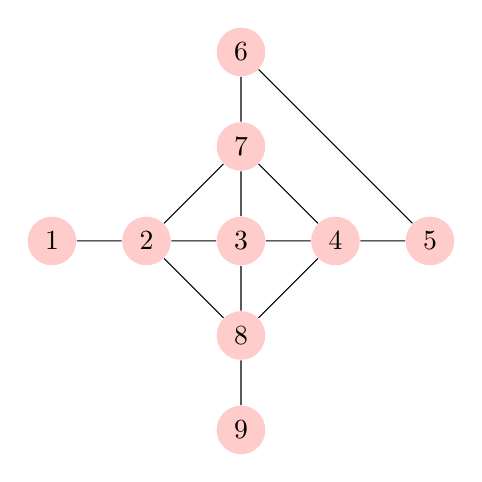
\begin{tikzpicture}
  [scale=.6,auto=left,every node/.style={circle,fill=red!20}]
  \node (n1) at (1,7) {1};
  \node (n2) at (3,7)  {2};
  \node (n3) at (5,7)  {3};
  \node (n4) at (7,7) {4};
  \node (n5) at (9,7)  {5};
  \node (n6) at (5,11)  {6};
   \node (n7) at (5,9) {7};
   \node (n8) at (5,5) {8};
   \node (n9)  at (5,3) {9};
  \foreach \from/\to in {n1/n2,n2/n3,n3/n4,n4/n5,n6/n7,n7/n3,n3/n8,n8/n9,n2/n7,
  n4/n7,n4/n8,n8/n2,n6/n5}
    \draw (\from) -- (\to);

\end{tikzpicture}
\caption{ Example Graph with 9 vertices and 13 edges}\label{4g2}
\end{center}
\end{figure}

\begin{figure}
\begin{center}
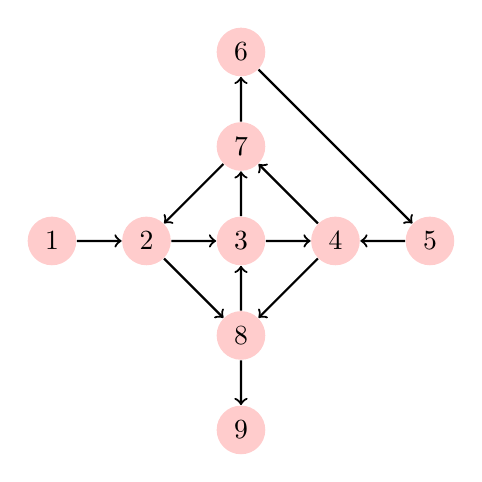
\begin{tikzpicture}
  [scale=.6,auto=left,every node/.style={circle,fill=red!20}]
  \node (n1) at (1,7) {1};
  \node (n2) at (3,7)  {2};
  \node (n3) at (5,7)  {3};
  \node (n4) at (7,7) {4};
  \node (n5) at (9,7)  {5};
  \node (n6) at (5,11)  {6};
   \node (n7) at (5,9) {7};
   \node (n8) at (5,5) {8};
   \node (n9)  at (5,3) {9};
 \path [->,draw,thick] 
  (n1) edge  (n2)
  (n2) edge (n3)
  (n3) edge (n4)
  (n4) edge (n8)
  (n8) edge (n3)
  (n3) edge (n7)
  (n7) edge (n6)
  (n6) edge (n5)
  (n5) edge (n4)
  (n4) edge (n7)
  (n7) edge (n2)
  (n2) edge (n8)
  (n8) edge (n9)
;
\end{tikzpicture}
\caption{ Eulerian walk from vertex 1 to vertex 9  1-2-3-4-8-3-7-6-5-4-7-2-8-9 of Figure \ref{4g2}}\label{4g25}
\end{center}
\end{figure}

\vspace{3in}
Rishnak asked Ajur how he would modify the graph shown in Figure \ref{4g2} to have a closed Eulerian Walk. Ajur reasoned that there are exactly two vertices of odd degrees, namely, vertices 1 and 9. If we were to join an edge between 1 and 9, then every vertex would have an even degree and hence a closed Eulerian Walk and that walk will be 1-2-3-4-8-3-7-6-5-4-7-2-8-9-1. Ajur also drew a graph.
as in Figure \ref{4g255}.
\begin{figure}
\begin{center}
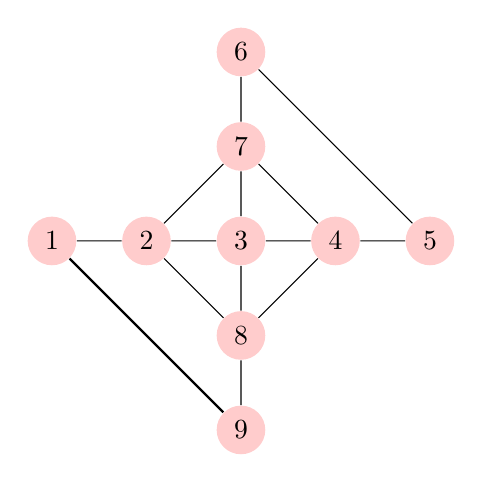
\begin{tikzpicture}
  [scale=.6,auto=left,every node/.style={circle,fill=red!20}]
  \node (n1) at (1,7) {1};
  \node (n2) at (3,7)  {2};
  \node (n3) at (5,7)  {3};
  \node (n4) at (7,7) {4};
  \node (n5) at (9,7)  {5};
  \node (n6) at (5,11)  {6};
   \node (n7) at (5,9) {7};
   \node (n8) at (5,5) {8};
   \node (n9)  at (5,3) {9};
  \foreach \from/\to in {n1/n2,n2/n3,n3/n4,n4/n5,n6/n7,n7/n3,n3/n8,n8/n9,n2/n7,
  n4/n7,n4/n8,n8/n2,n6/n5}
    \draw (\from) -- (\to);
\path[thick] (n1) edge (n9);
\end{tikzpicture}
\caption{ Closed Eulerian Walk with edge (1,9) added to Figure \ref{4g2}}\label{4g255}
\end{center}
\end{figure}

Rishnak asked how he would modify the graph shown in Figure \ref{4g1} to have a closed Eulerian walk. Ajur now had a problem. The two vertices which have odd degrees, 2 and 4, already have an edge between them. However, he remembered the definition of a \emph{multigraph}, where there may be multiple edges between any given pair of vertices. So he added another edge between 2 and 4 and exclaimed that there is a closed Eulerian walk 2-3-4-1-2-4-2. Ajur again drew a graph as shown in Figure \ref{4g155}
%Ajur added that if a graph is not connected, there is neither Eulerian walk nor a closed Eulerian walk (as there is no walk from some vertex to some other vertex - In an Eulerian walk,.
\begin{figure}
\begin{center}
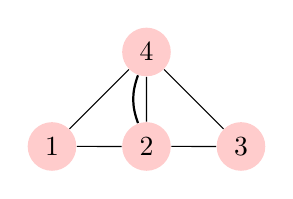
\begin{tikzpicture}
  [scale=.6,auto=left,every node/.style={circle,fill=red!20}]
  \node (n1) at (1,7) {1};
  \node (n2) at (3,7)  {2};
  \node (n3) at (5,7)  {3};
  \node (n4) at (3,9)  {4};

  \foreach \from/\to in {n1/n2,n2/n3,n2/n4,n1/n4,n3/n4}
    \draw (\from) -- (\to);
\path[thick] (n2) edge[bend left=20] (n4);
\end{tikzpicture}
\caption{ Graph in Figure \ref{4g1} with edge (2,4) added to have a closed Eulerian Walk}\label{4g155}
\end{center}
\end{figure}

\vspace{3in}
Rishnak then asked Ajur whether he knew about multi graphs and directed graphs. Ajur realized he essentially learnt about multigraphs  by doing the Eulerian walks and completion  example. \textbf{which example is the completion example?} Ajur added that in a directed graph an edge $(x,y)$ goes from vertex $x$ to $y$ and he drew an example graph to show Rishnak that he understood. See Figure \ref{4g5}. 
Ajur mentioned that instead of \emph{the} degree of a vertex, there is an in-degree and an out-degree of a vertex. The number of edges coming to a vertex is the in-degree of that vertex and the number of edges going out of a vertex is the out-degree of a vertex. For example, in the directed graph shown in Figure \ref{4g5}, vertex 1 has in-degree 2 and out-degree 1. Each of Vertex 3 and 4 has in-degree  and out-degree 1. A directed graph is strongly connected if there is a directed path from every vertex to every other vertex. For example, the directed graph shown in Figure \ref{4g5} is strongly connected. Rishnak said that an Eulerian walk will only exist on strongly connected directed graphs.

\begin{figure}
\begin{center}
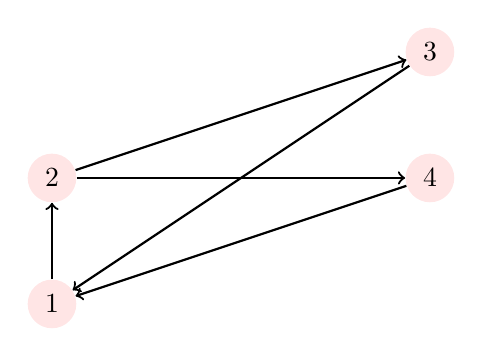
\begin{tikzpicture}
  [scale=.8,auto=left,every node/.style={circle,fill=red!10}]
  \node (n1) at (1,7) {1};
  \node (n2) at (1,9)  {2};
  \node (n3) at (7,11)  {3};
  \node (n4) at (7,9) {4};
 \path[->, draw,thick] 
        (n1) edge (n2)
         (n3) edge (n1)
        (n2) edge (n3)
        (n2) edge (n4)
        (n4) edge  (n1);

\end{tikzpicture}
\caption{ Example Directed Graph with 4 vertices and 5 edges}\label{4g5}
\end{center}
\end{figure}


Anticipating Rishnak's question, Ajur responded that there was no closed Eulerian walk in this directed graph. Rishnak reminded Ajur that he wanted to know whether there was an Eulerian walk from vertex 2 to vertex 1. Ajur reasoned in a  manner similar to before. Ajur saw a directed cycle (1,(1,2),2,(2,3),3,(3,1),1) or simply (1,2,3,1). So Ajur was able to write the Eulerian walk as 2-3-1-2-4-1. Ajur said to have a closed Eulerian walk, you should have a collection of edge-disjoint cycles (no edge is common between these cycles). In such a case, the in-degree of each vertex should be the same as its out-degree (this is related to the condition for an undirected graph to admit an Eulerian cycle: the degree of every vertex has to be an even number). For an Eulerian walk, it has to start from a vertex which has one more out-degree than in-degree and end in a vertex which has one more in-degree than out-degree (For all other vertices, the in-degree should be equal to the out-degree).

It was getting late - but Rishank wanted to share several exciting applications of Eulerian walks. 

Consider the following problem: construct a string of 0's and 1's such that all four two-bit strings occur as a substring (there are 4 two-bit strings consisting of 0's and 1's: 00,01,10 and 11). For example in the string 00110, all two-bit strings occur. Suppose instead we wanted to build a \emph{circular} string that contained all two-bit substrings. Such a string is known as DeBruijn sequence. Rishnak added that this problem is closely related to constructing a closed Eulerian walk. If we construct an Eulerian walk on the directed graph of Figure \ref{4g55}, we would get such a string.

For this directed graph, there are two vertices with labels 0 and 1. There is a directed edge with label 0 from vertex labeled 0 to itself. There is a directed edge with a label 1 from the vertex labeled 0 to the vertex labeled 1. (The idea behind the first edge is to consider appending 0 (the edge label) to 0 (the starting vertex label) to get 00. Then omit the first character 0. The result is 0 which is the vertex labeled 0 - hence a self loop). \textbf{This last part is somewhat unclear...can you rewrite it?} Similarly there is an edge with a label 1 from a vertex labeled 1 to itself and there is a vertex an edge with 
a label 0 from vertex labeled 1 to a vertex labeled 0.
Each vertex has an in-degree of 2 and an out-degree if 2. Hence it has a closed Eulerian walk from the vertex labeled 0 to itself and that walk is 0110 (here, each character is an \emph{edge label}!) From this, we get all the four substrings of length 2, namely 01,11,10,00 (the last one is taking the last character and the first character as it is a closed walk).

\begin{figure}
\begin{center}
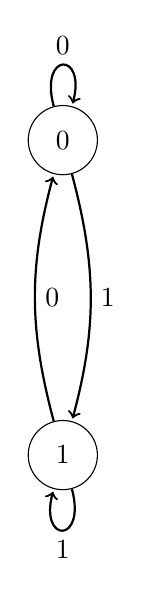
\begin{tikzpicture}[shorten >=1pt,node distance=4cm,on grid,auto] 
 
   \node[state] (q_1)  {$0$}; 
   \node[state] (q_2) [below =of q_1] {$1$}; 
    \path[->,draw,thick] 
    
    (q_1) edge [bend left=15] node  {1} (q_2)
          edge [loop above] node {0} ()
    (q_2) edge [bend left=15] node [swap] {0} (q_1) 
          edge [loop below] node {1} ();
   
\end{tikzpicture}
\caption{ An Eulerian walk on this directed graph will yield a DeBruijn sequence that contains  all substrings of length 2 over a binary alphabet 0 and 1}\label{4g55}
\end{center}
\end{figure}
Rishnak then asked Ajur to construct a DeBruijn Sequence that contains all substrings of length 3.
Ajur thought that the question was to obtain a string 0's and 1's such that all eight three-bit strings occur as a substring; the 8 three bit strings consisting of 0's and 1's are 
$$000, 001, 010, 011, 100, 101, 110, 111.$$ Ajur wanted to construct a graph from which an Eulerian walk would naturally yield such a sequence. 

Consider a directed graph with 4 vertices, labeled 00, 01, 10 and 11.
There is an edge from vertex labeled 00 to itself with a label 0 (if you get a 0, you append 0 to the vertex label (00) and drop the first character). There is an edge with label 1 from
vertex labeled 00 to a vertex labeled 01. Vertex labeled 00 has an out-degree of 2. Similarly there is an edge with label 0 from vertex labeled 01 to vertex with label 10. There is an edge with label 1 from vertex labeled 01 to vertex with label 11. 


\textbf{For the next paragraph you could cut the rest of the description and just go to the graph} We continue to build the graph following the natural pattern. Draw an edge with label 0 from a  vertex labeled 10 to a vertex labeled 00. Draw an edge with label 1 from a vertex labeled 10 to a vertex labeled 01.
Draw an edge with label 0 from a vertex labeled 11 to a vertex labeled 10. Draw an edge with label 1 from a vertex labeled 11 to itself.
The resulting directed graph is as shown in Figure \ref{4g6}. An Eulerian walk starting from a vertex labeled 00 is $0 1 0 1 1 1 0 0$  (We start with a vertex labeled 00 and the label of the edges traversed in an Eulerian Walk). This walk is also a closed Eulerian Walk as we start and end with the same vertex (labeled $00$).
From the walk, we get all the strings of length 3 (over 0 and 1) as substrings in the Eulerian Walk.
001, 010,101,011,111,110,100 and 000 (000 by knowing this is a closed Eulerian walk and we get 000, by taking two characters and the first character of the Eulerian Walk.).\\
\vspace{0.2in}
\begin{figure}
\begin{center}
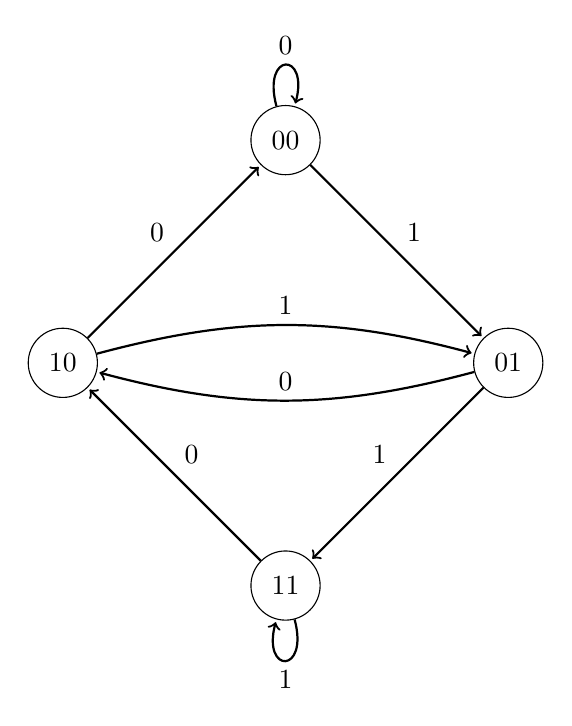
\begin{tikzpicture}[shorten >=1pt,node distance=4cm,on grid,auto] 
   \node[state] (q_0)   {$10$}; 
   \node[state] (q_1) [above right=of q_0] {$00$}; 
   \node[state] (q_2) [below right=of q_0] {$11$}; 
   \node[state](q_3) [below right=of q_1] {$01$};
    \path[->,draw,thick] 
    (q_0) edge  node {0} (q_1)
          edge [bend left=15] node  {1} (q_3)
    (q_1) edge  node  {1} (q_3)
          edge [loop above] node {0} ()
    (q_2) edge  node [swap] {0} (q_0) 
          edge [loop below] node {1} ()
    (q_3) edge [bend left=15] node [swap] {0} (q_0) 
          edge  node [swap] {1} (q_2);
\end{tikzpicture}
\caption{ An Eulerian walk on this directed graph will yield a DeBruijn sequence that contains all substrings of length 3 over a binary alphabet 0 and 1}\label{4g6}
\end{center}
\end{figure}
%\vspace{0.1in}
%\noindent

Rishnak said that another application of Eulerian Walk is in the creation of mazes or labyrinths (as known in Greece) or bhul bulaiyah (as known in India).  It is easy to enter a maze but it is difficult to get out of one. There are large walls which prevent one from seeing where the corridors lead to. Rishnak told Ajur that there were reports of people dying in mazes because they were unable to find their way out. One was the angel Kinaja who was a human trapped in a maze. She had figured out how to get out but was too exhausted to walk and died. Kinaja had told Rishnak people who studied graph theory and understood Eulerian walks could find their way out of a maze. Jura said he knew too about mazes, having seen a YouTube video of a psychology lab experiment with mice running in a maze. Jura had also been in one as a child when his parents took him to a corn field maze. Ajur was also eager to show off his knowledge of poetry and quoted from Robert Frost's poem \emph{The Road not Taken} which is related to traversing a maze: \begin{quotation}\noindent Two roads diverged in a wood, and I--\\ 
I took the one less traveled by,\\ And that has made all the difference.
\end{quotation}

\noindent Rishnak was getting impatient, as poltergeists tend to, and he wanted to stay focused on the maze. Rishnak showed his two friends a picture of the maze in Figure \ref{4g7}.
\begin{figure}
\begin{center}
\includegraphics{maze11.jpg}
\caption{A Maze with a start and goal and intermediate vertices marked for clarity}\label{4g7}
\end{center}
\end{figure}

He said that one could construct a graph from the maze by putting a vertex at each place where there is an open space in the wall or where you have choices to make it. \textbf{Can you clarify construction of the maze in this text?} Join the vertices if there is a corridor connecting them (and there are no vertices between them). This will result in a tree (no cycle will be present). Now you can make this graph Eulerian by going over each edge twice. One uses bread crumbs to mark the edge traversed. If an edge has two bread crumbs, that means you don't traverse that edge any more.

That was precisely the strategy Kinaja had told Rishank for one to get out of the maze.  In the beginning all the paths are free of bread crumbs. When ever one takes a path (if there are bread crumb free paths available), you put bread crumbs along that edge; and if there are no bread crumb free paths are available, take the path in which there is only one bread crumb present and walk through that path putting bread crumbs. Eventually you will reach the end goal as there is an Eulerian walk present in the underlying graph of the maze. \textbf{I don't exactly understand this: can you rewrite it?}

\begin{figure}
\begin{center}
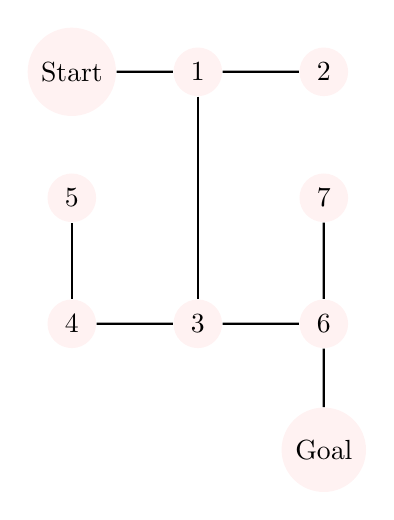
\begin{tikzpicture}
[scale=.8,auto=left,every node/.style={circle,fill=red!5}]
   \node (q_0)   at (1,7) {Start}; 
   \node (q_1) at  (3,7) {1}; 
   \node (q_2) at (5, 7) {2}; 
   \node(q_3) at (3,3) {3};
   \node (q_4) at (1,3) {4};
   \node (q_5) at (1,5) {5};
   \node(q_6) at (5,3) {6};
   \node(q_7) at (5,5) {7};
   \node(q_8) at (5,1) {Goal};
    \path[-,draw,thick] 
    (q_0) edge   (q_1)
    (q_1) edge (q_2)
    (q_1) edge (q_3)
    (q_3) edge  (q_4)
    (q_4) edge (q_5)
    (q_3) edge (q_6)
    (q_6) edge (q_7)
    (q_6) edge (q_8);

\end{tikzpicture}
\caption{ A graph/tree of Figure \ref{4g7}}\label{4g8}
\end{center}
\end{figure}

Ajur took another maze and in that he drew the graph Figure \ref{4g9} to show Rishnak that he has understood.

\begin{figure}
\begin{center}
\includegraphics{anothermaze.jpg}
\caption{A Maze with a Start and Goal and the graph drawn inside the maze}\label{4g9}
\end{center}
\end{figure}
Ajur was truly impressed by the power of Eulerian walk and he wanted a walk named after himself too! The sun was setting and it was time to go to go home.
\chapter{Hamiltonian Path/Cycle}
Ajur was walking with Jura thinking what he could do to inspire a problem to be named after himself. Rishnak found Ajur to be an interesting youngster to discuss puzzles based on Graph Theory. After the discussion of the Eulerian Walk, Rishnak decided to introduce a closely related graph-theoretic construction: Hamiltonian Paths and Hamiltonian Cycles. Rishank approached Ajur and Jura and began defining the notion of a Hamiltonian path and Hamiltonain walk.
In a Hamiltonian path each of the vertices are visited exactly once. 
The length of a path is the number of edges in that path. A Hamiltonian path in a graph with $n$ vertices will have a path length of $n-1$. A Hamiltonian cycle is a cycle that visits each vertex once and only once. The length of a Hamiltonian Cycle in a graph with $n$ vertices is $n$. Rishnak asked Ajur whether there is a Hamiltonian cycle in the graph of Figure \ref{5g1},
\begin{figure}
\begin{center}
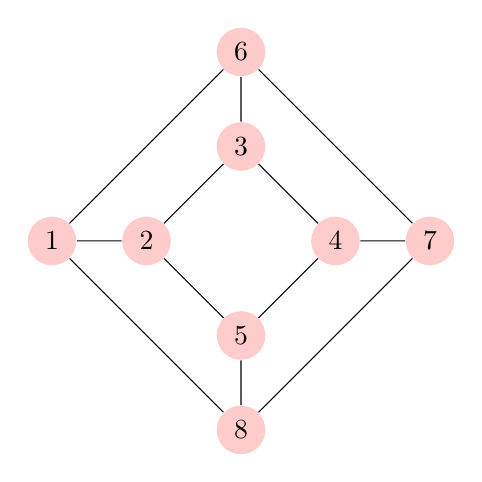
\begin{tikzpicture}
  [scale=.6,auto=left,every node/.style={circle,fill=red!20}]
  \node (n1) at (1,7) {1};
  \node (n2) at (3,7)  {2};
  \node (n4) at (7,7) {4};
  \node (n7) at (9,7)  {7};
  \node (n6) at (5,11)  {6};
   \node (n3) at (5,9) {3};
   \node (n5) at (5,5) {5};
   \node (n8)  at (5,3) {8};
  \foreach \from/\to in {n1/n2,n2/n3,n3/n4,n4/n5,n5/n2,n1/n6,
  n6/n7, n7/n8, n8/n1, n3/n6, n4/n7, n5/n8}
    \draw (\from) -- (\to);

\end{tikzpicture}
\caption{ Cube Graph }\label{5g1}
\end{center}
\end{figure}

Ajur thought about for a few seconds and he drew the Hamiltonian cycle of Figure \ref{5g1} in Figure \ref {5g2}. Krishnak told Ajur that his solution is not unique and there are more solutions!\footnote{Try to find a Hamiltonian Cycle distinct from the one described by Ajur!}

\begin{figure}
\begin{center}
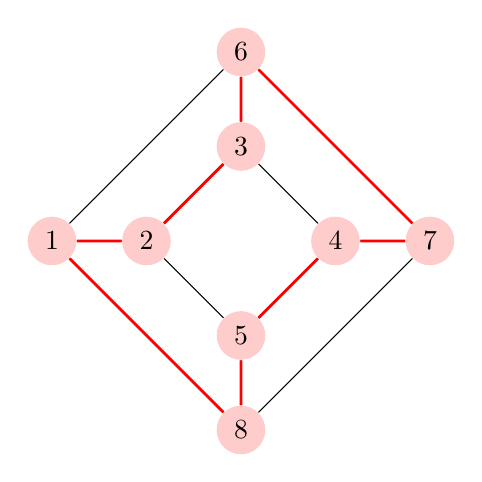
\begin{tikzpicture}
  [scale=.6,auto=left,every node/.style={circle,fill=red!20}]
  \node (n1) at (1,7) {1};
  \node (n2) at (3,7)  {2};
  \node (n4) at (7,7) {4};
  \node (n7) at (9,7)  {7};
  \node (n6) at (5,11)  {6};
   \node (n3) at (5,9) {3};
   \node (n5) at (5,5) {5};
   \node (n8)  at (5,3) {8};
  \foreach \from/\to in {n1/n2,n2/n3,n3/n4,n4/n5,n5/n2,n1/n6,
  n6/n7, n7/n8, n8/n1, n3/n6, n4/n7, n5/n8}
    \draw (\from) -- (\to);
\path[line width=0.35mm,red] (n1) edge (n2)
(n2) edge (n3)
(n3) edge (n6)
(n6) edge (n7)
(n7) edge (n4)
(n4) edge (n5)
(n5) edge (n8)
(n8) edge (n1);
\end{tikzpicture}
\caption{ Cube Graph with Hamiltonian  Cycle marked in thick edges}\label{5g2}
\end{center}
\end{figure}

Rishnak then told Ajur what led Hamilton to the statement of the Hamiltonian cycle problem. The mathematician Hamilton wanted a cycle to visit 
all the vertices of a dodecahedron (one of the five platonic solids) which has 20 vertices and 30 edges. 
Rishnak asked Ajur whether there is a Hamiltonian Cycle in the graph of Figure \ref{5g3}. Rishnak added that this is a well-known graph, called the Petersen Graph.

\begin{figure}
\begin{center}
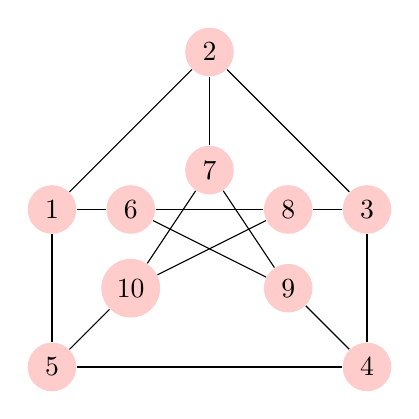
\begin{tikzpicture}
  [scale=.5,auto=left,every node/.style={circle,fill=red!20}]
  \node (n1) at (1,7) {1};
  \node (n2) at (5,11)  {2};
  \node (n3) at (9,7)  {3};
  \node (n4) at (9,3) {4};
  \node (n5) at (1,3) {5};
  \node (n6) at (3,7)  {6};
  \node (n7) at (5,8) {7};
  \node (n8)  at (7,7) {8};
  \node (n9) at (7,5) {9};
  \node (n10) at  (3,5) {10};
 
  \foreach \from/\to in {n1/n2,n2/n3,n3/n4,n4/n5,n5/n1,n1/n6,
  n2/n7, n3/n8, n4/n9, n5/n10, n6/n8, n8/n10, n10/n7,n7/n9,n9/n6}
    \draw (\from) -- (\to);

\end{tikzpicture}
\caption{ Petersen Graph with 10 vertices and 15 edges }\label{5g3}
\end{center}
\end{figure}
Ajur thought for a while and he was not able to construct a Hamiltonian cycle. He however, was able to find a 
Hamiltonian path. So he drew the following Figure \ref{5g4}. Rishnak mentioned to Ajur that this Hamiltonian path is not unique and there are other Hamiltonian paths.\footnote{Find a Hamiltonian path distinct from the one shown here.}


\begin{figure}
\begin{center}
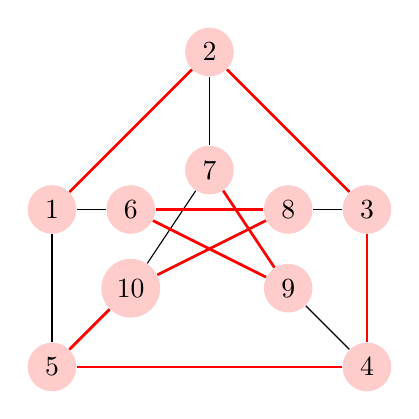
\begin{tikzpicture}
  [scale=.5,auto=left,every node/.style={circle,fill=red!20}]
  \node (n1) at (1,7) {1};
  \node (n2) at (5,11)  {2};
  \node (n3) at (9,7)  {3};
  \node (n4) at (9,3) {4};
  \node (n5) at (1,3) {5};
  \node (n6) at (3,7)  {6};
  \node (n7) at (5,8) {7};
  \node (n8)  at (7,7) {8};
  \node (n9) at (7,5) {9};
  \node (n10) at  (3,5) {10};
 
  \foreach \from/\to in {n1/n2,n2/n3,n3/n4,n4/n5,n5/n1,n1/n6,
  n2/n7, n3/n8, n4/n9, n5/n10, n6/n8, n8/n10, n10/n7,n7/n9,n9/n6}
    \draw (\from) -- (\to);
\path[line width=0.35mm,red]
(n1) edge (n2)
(n2) edge (n3)
(n3) edge (n4)
(n4) edge (n5)
(n5) edge (n10)
(n10) edge (n8)
(n8) edge (n6)
(n6) edge (n9)
(n9) edge (n7);

\end{tikzpicture}
\caption{ Petersen Graph with a Hamiltonian Path}\label{5g4}
\end{center}
\end{figure}
Rishnak assured Ajur that Petersen Graph indeed does not have a Hamiltonian cycle. Whether a graph has an Eulerian Cycle or not can easily be tested (the degree of every vertex has to be even), however, there is no easy way for test whether a given graph has a Hamiltonian cycle. 

Rishnak continued that there is a special class of graphs called bipartite graphs where every cycle is of even length. The vertex set can be partitioned into two sets $A$ and $B$, such that every edge in such a graph has one end vertex in $A$ and the other end vertex in $B$. Rishnak showed an example Figure \ref{5g5}. Ajur immediately said that all the cycles are of even lengths (4 and 6).\footnote{Every edge in the cycle must go from one partition to the other partition (as they are the only possible edges). Hence the length of a cycle must be even.} Rishnak asked Ajur what the two vertex partitions are (all the edges go from one partition to the other). After a little thought Ajur said one partition contains 1, 3, 5 and the other partition contains the vertices 2, 4 and 6. Ajur drew a graph (see Figure \ref{5g55}) to illustrate  what he meant. Ajur also mentioned that this graph has a Hamiltonian cycle.\footnote{Ajur exclaimed that every tree is a bipartite graph too, as a tree contains no cycles (or cycles of length 0 - we know that 0 is an even number!). Rishnak reminded Ajur that since tree does not have cycles and hence no Hamiltonian cycles.} 
Ajur wanted to show that he had understood the concept of a bipartite graph. So he drew a graph that does not have a Hamiltonian cycle - see Figure \ref{5g6}. Ajur explained why this graph does not have a Hamiltonian cycle. If there were a Hamiltonian cycle, the vertices in the cycle have to alternate between the two vertex partitions. But one vertex partition has two vertices and the other vertex partition has three vertices. Rishnak smiled and appreciated Ajur's logical thinking.

\begin{figure}
\begin{center}
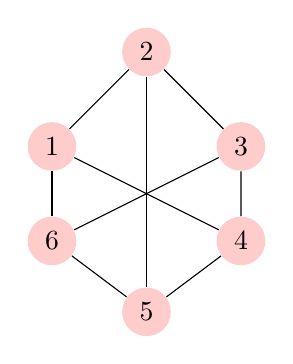
\begin{tikzpicture}
  [scale=.3,auto=left,every node/.style={circle,fill=red!20}]
  \node (n1) at (1,7) {1};
  \node (n2) at (5,11)  {2};
  \node (n3) at (9,7)  {3};
  \node (n4) at (9,3) {4};
  \node (n5) at (5,0)  {5};
  \node (n6) at (1,3) {6};
  
   \foreach \from/\to in {n1/n2,n2/n3,n3/n4,n4/n5,n5/n6,n1/n6,
  n2/n5, n6/n3,n1/n4}
    \draw (\from) -- (\to);
    \end{tikzpicture}
\caption{ A Bipartite Graph with 6 vertices and 9 edges}\label{5g5}
\end{center}
\end{figure}
\begin{figure}
\begin{center}
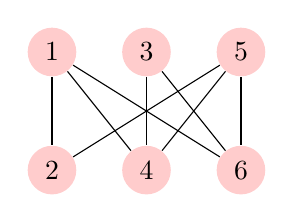
\begin{tikzpicture}
  [scale=.3,auto=left,every node/.style={circle,fill=red!20}]
  \node (n1) at (1,7) {1};
  \node (n3) at (5,7)  {3};
  \node (n5) at (9,7) {5};
  \node (n2) at (1,2)  {2};
  \node (n4) at (5,2) {4};
  \node (n6) at (9,2)  {6};
 
  
   \foreach \from/\to in {n1/n2,n1/n4,n1/n6,n3/n4,n3/n6,n5/n2,n5/n4,n5/n6}
    \draw (\from) -- (\to);
    \end{tikzpicture}
\caption{ Graph in \ref{5g5} drawn with vertex partition}\label{5g55}
\end{center}
\end{figure}
\begin{figure}
\begin{center}
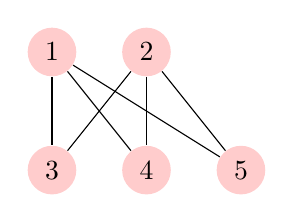
\begin{tikzpicture}
  [scale=.3,auto=left,every node/.style={circle,fill=red!20}]
  \node (n1) at (1,7) {1};
  \node (n2) at (5,7)  {2};
  \node (n3) at (1,2)  {3};
  \node (n4) at (5,2) {4};
  \node (n5) at (9,2)  {5};
 
  
   \foreach \from/\to in {n1/n3,n1/n4,n1/n5,n2/n3,n2/n4,n2/n5}
    \draw (\from) -- (\to);
    \end{tikzpicture}
\caption{ A Bipartite Graph with 5 vertices and 6 edges}\label{5g6}
\end{center}
\end{figure}

Rishnak decided to tell Ajur a simplified version of a puzzle\footnote{attributed to Bruce Robinson, a professor of civil and environmental engineering at the University of Tennessee} he had heard in the radio program Car Talk (broadcast on public radio). There are 9 jealous people who live in the squares of a three-by-three grid (see Figure \ref{5g7}. The squares are numbered, starting on the upper left-hand corner, 1 through 9 (first going across). Each person is jealous of his adjacent neighbor; we emphasize not his diagonal neighbor, but only the people above or below or to the right or to the left of him. Each aspires to move into the apartment of an adjacent neighbor.
The question is very simple: What is the fewest number of total moves that can accomplish this?
\begin{figure}
\begin{center}
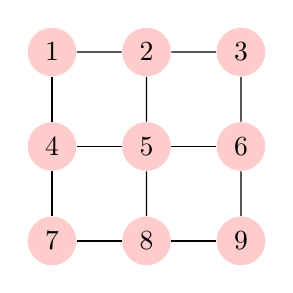
\begin{tikzpicture}
  [scale=.3,auto=left,every node/.style={circle,fill=red!20}]
  \node (n1) at (1,11) {1};
  \node (n2) at (5,11)  {2};
  \node (n3) at (9,11) {3};
  \node (n4) at (1,7)  {4};
  \node (n5) at (5,7) {5};
  \node (n6) at (9,7)  {6};
  \node (n7) at (1,3)  {7};
  \node (n8) at (5,3) {8};
  \node (n9) at (9,3)  {9};
  
  
   \foreach \from/\to in {n1/n2,n1/n4,n2/n3,n2/n5,n3/n6,n4/n5,n4/n7,n5/n6,n5/n8,n6/n9,n7/n8,
   n8/n9}
    \draw (\from) -- (\to);
    \end{tikzpicture}
\caption{ A three by three grid with nine apartments. Apartments are modeled as vertices and an edge denotes adjacency relation between apartments (up, down, two sides - not all apartments have all of the adjacent apartments} \label{5g7}
\end{center}
\end{figure}

Ajur immediately figured  this is a bipratite graph and the partitions are not of equal size. Hence immediately he responded that this is not possible. Rishnak asked Ajur to write down the argument to make sure it is correct. Ajur promised that he would do it by next day. This graph has a Hamiltonian path but not a Hamiltonian cycle. Ajur said that instead of three by three grid of apartments, if we had a four by three grid (or three by four grid) of apartments, it is easy for all of them to transfer to the adjacent apartments. Such a graph has a Hamiltonian cycle. \textbf{why?}

Rishnak continued with other related puzzles. Euler proposed the \emph{Knight's tour} problem on a chessboard. A chessboard is an eight by eight square grid. Place a knight in any square. From that square, the knight has to move\footnote{knight may only move either two squares vertically up/down and one square horizontally left or right or one square vertically up or down and two squares horizontally left or right. More coloquially, a knight moves in a 2x1 L shape} visiting all of the squares squares exactly. One may think of this as finding a Hamiltonian path in a 64-vertex graph with two vertices adjacent if there is a knight move from one vertex to the other. There is no easy method of finding a knight's tour other than exhaustive search.\footnote{The usual method of exhaustive search is through backtracking - a systematic method of exploring all possibilities.} Here is a solution in Table \ref{5t1} for a five by five chess board with the knight's tour starting from bottom left.
\begin{table}
\centering
\begin{tabular}{|c |c |c| c| c|} 
 \hline
3&10&21&16& 5\\
\hline
20&15& 4&11&22\\
\hline
 9& 2&23& 6&17\\
 \hline
14&19& 8&25&12\\
\hline
 1&24&13&18& 7\\
 \hline
\end{tabular}
\caption{Knight's Tour on five by five chess board starts at the bottom left}
\label{5t1}
\end{table}
Rishnak asked Ajur to find the message is encoded here in Table \ref{5t2}.
\begin{table}
\centering
\begin{tabular}{c c c c cc}
i& t& t& t& b& l\\
r& h &d &e& u& s\\
h& a& y& e& d& o\\
a& o& e& p& r& n\\
s& n& f& o& l& l\\
f& v& d &i& e& u\\
\end{tabular}
\caption{What is the Message is encoded here}
\label{5t2}
\end{table}
Rishnak added that there are poems from different cultures (including India and China) based on Knight's tour. Ajur was intrigued and resolved to read and understand the poems. Rishnak added that one needs to verify that a knight's tour is impossible for a three by three chessboard or a four by four chessboard and warned that checking whether a knight's tour is impossible may take a long time.

There are many methods to check whether a given graph has a Hamiltonian cycle. Unfortunately these conditions are \textbf{not} exhaustive. Rishnak taught Ajur a simple test to know whether a graph has a Hamiltonian cycle.

Rishnak stated a well-known theorem that if the degree of every vertex in a graph with $n$ vertices is at least$\frac{n}{2}$, then the graph has a Hamiltonian cycle. The main proof argument consists of three parts.
\begin{enumerate}
    \item The graph is connected.
    \item If one gives the longest path, one can find a Hamiltonian cycle or the given path is not the longest path.
    \item Every graph has a longest path with a path length of $\le n-1$.
\end{enumerate}


First the graph has to be connected - Otherwise there will be at least two connected components, one of which will have size at most $\frac{n}{2}$, violating the degree condition. In this connected graph, find the longest path. Let it be $v_1,v_2,\cdots, v_k$. Since this is the longest path, all the neighbors of the starting vertex $v_1$ and the ending vertex $v_k$ have  to be in this path. Otherwise we could have extended that path and hence the path we started with is not the longest path. Hence at least $\frac{n}{2}$ vertices in the path $v_2,v_3,\cdots,v_k$ are adjacent to $v_0$. Let those adjacent vertices of $v_1$ be a set $S_1$= $\{v_i,v_j,\cdots v_m\}$. The size of this set is at least $\frac{n}{2}$. For each of these vertices, consider their preceding vertices in the Path. Let that set be $S_2$. The size of that set is also $\frac{n}{2}$. The vertices adjacent $v_k$ has to be of size $\frac{n}{2}$ and they are among $v_1,v_2,\cdots v_{k-1}$. If none of the vertices adjacent to $v_k$ are in set $S_2$, then the vertices adajcent to $v_k$ will be size < $\frac{n}{2}$ because $k-1-\frac{n}{2} <\frac{n}{2}$. Hence we will have a situation as shown in Figure \ref{5g100}
\begin{figure}
\begin{center}
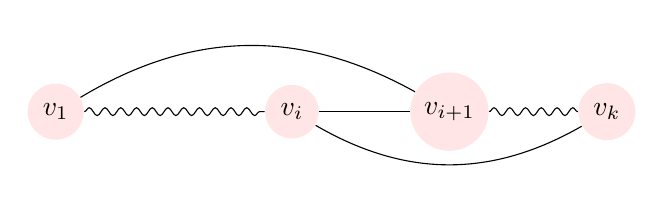
\begin{tikzpicture}
  [scale=.5,auto=left,every node/.style={circle,fill=red!10}]
  \node (n1) at (-1,11) {$v_1$};
  \node (n2) at (5,11)  {$v_i$};
  \node (n3) at (9,11) {$v_{i+1}$};
  \node (n4) at (13,11) {$v_k$};
  
  

    \draw (n2) -- (n3);
   \path (n1) edge[bend left=30] (n3);
    \path (n2) edge[bend right=30] (n4);
    \tikzset{decoration={snake,amplitude=.5mm,segment length=2mm,
                       post length=0mm,pre length=0mm}}
  \draw[decorate] (n1) -- (n2);
  \draw[decorate] (n3) -- (n4);
    \end{tikzpicture}
\caption{ Pictorial Description of the argument; solid lines represent edges, squiggly lines represent paths} \label{5g100}
\end{center}
\end{figure}
 
This creates a cycle $v_k,v_i,\cdots,v_1,v_{i+1}\cdots, v_k$ as shown in \ref{5g100}. Claim is that this is a Hamiltonian Cycle. If not there is at least one vertex in this cycle that will be adjacent to some other vertex. This will result in a path longer than the path we originally started - a contradiction.
Ajur was able to follow along and loved the subtle and the clever arguments used in the proof. But Jura who was patiently waiting was beginning to get restless so Ajur called it a day.

\chapter{Graph Isomorphism, Subgraph Isomorphism}

Rishnak was eagerly looking for Ajur because he wanted to share with him a new concepts and found Ajur and Jura walking along the bank of a (presumably haunted) pond in the cemetery. Rishnak started this session with a small variant on what they had been discussing. A graph whose vertices are labeled is called a labeled graph and one without labels for vertices is called an unlabeled graph. Two labeled graphs are equivalent if they are identical. The labeled graphs in Figures \ref{8g1} and \ref{8g11} are equivalent. The graph in Figure \ref{8g2} is not equivalent to the graph in Figures \ref{8g1} or \ref{8g11} or  \ref{8g2} as there is no edge between vertices 4 and 5.
\begin{figure}
\begin{center}
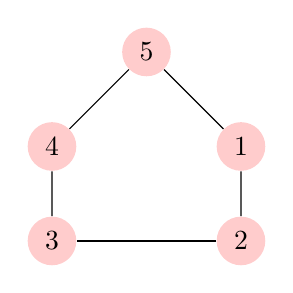
\begin{tikzpicture}
  [scale=.6,auto=left,every node/.style={circle,fill=red!20}]
  \node (n1) at (5,5) {1};
  \node (n4) at (1,5)  {4};
  \node (n3) at  (1,3) {3};
  \node (n2) at (5,3)  {2};
  \node (n5) at (3,7)  {5};

  \foreach \from/\to in {n1/n2,n2/n3,n3/n4,n4/n5,n1/n5}
    \draw (\from) -- (\to);

\end{tikzpicture}
\caption{Labeled Graph}\label{8g1}
\end{center}

\end{figure}
\begin{figure}
\begin{center}
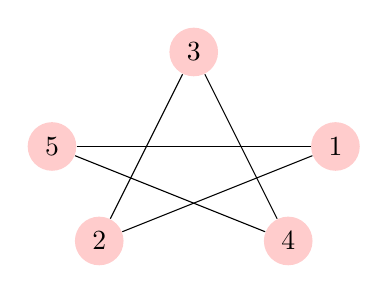
\begin{tikzpicture}
  [scale=.6,auto=left,every node/.style={circle,fill=red!20}]
   \node (n1) at (6,5) {1};
  \node (n5) at (0,5)  {5};
  \node (n2) at  (1,3) {2};
  \node (n4) at (5,3)  {4};
  \node (n3) at (3,7)  {3};

  \foreach \from/\to in {n1/n2,n2/n3,n3/n4,n4/n5,n5/n1}
    \draw (\from) -- (\to);

\end{tikzpicture}
\caption{ Another labeled graph with five vertices equivalent to Figure \ref{8g1}}\label{8g11}
\end{center}
\end{figure}

\begin{figure}
\begin{center}
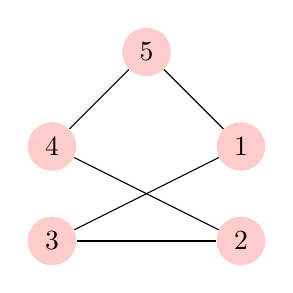
\begin{tikzpicture}
  [scale=.6,auto=left,every node/.style={circle,fill=red!20}]
   \node (n1) at (5,5) {1};
  \node (n4) at (1,5)  {4};
  \node (n3) at  (1,3) {3};
  \node (n2) at (5,3)  {2};
  \node (n5) at (3,7)  {5};


  \foreach \from/\to in {n1/n3,n2/n4,n3/n2,n1/n5,n5/n4}
    \draw (\from) -- (\to);

\end{tikzpicture}
\caption{ Another labeled graph with five vertices which is not equivalent to Graphs \ref{8g1} and \ref{8g11} as the edge labels are distinct from either of the two graphs}\label{8g2}
\end{center}
\end{figure}

Rishnak continued rhetoricaly: ``when are two graphs the same"? Two graphs are isomorphic (\emph{structurally the same}), if they are equivalent under a vertex relabeling. For example, if in the graph of Figure \ref{8g2} vertex 2 is relabeled as 3 and vertex 3 is relabeled as 2, then two graphs in Figures \ref{8g2} and \ref{8g1} are equivalent. If a graph, $G$, is equivalent to a graph $H$ and $H$ is equivalent to another graph $P$, then $G$ is equivalent to graph $P$\footnote{In other words, the relation of being equivalent graphs is transitive.}. To test whether two graphs are isomorphic are not is a hard problem\footnote{Not as hard as finding a Hamiltonian Cycle in a graph} .

If two graphs are isomorphic, they should have the same number of vertices, the same number of edges, the same degree sequences, the same length of the longest cycle, and the same length of the shortest cycle.  These properties of graphs are called graph invariants. By no mean are these invariants are exhaustive. We do not know of a single easily computable invariant that can be used to test whether or not two given graphs are isomorphic. 

Rishnak asked Ajur, to provide two graphs which have the same number of vertices and same number of edges but they are not isomorphic. Ajur thought a bit and he was able to produce the following two graphs which have 6 vertices and 9 edges. Ajur added that one graph is bipartite (all cycles are of even length) \ref{8g3} and the other one is not bipartite (it has cycle of length 3) \ref{8g4} and hence these two graphs are not isomorphic.

\begin{figure}

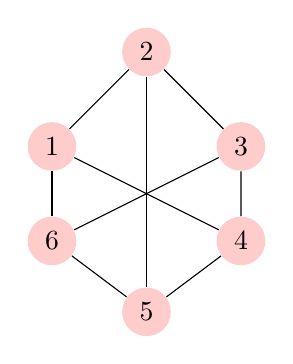
\begin{tikzpicture}
  [scale=.3,auto=left,every node/.style={circle,fill=red!20}]
  \node (n1) at (1,7) {1};
  \node (n2) at (5,11)  {2};
  \node (n3) at (9,7)  {3};
  \node (n4) at (9,3) {4};
  \node (n5) at (5,0)  {5};
  \node (n6) at (1,3) {6};
  
   \foreach \from/\to in {n1/n2,n2/n3,n3/n4,n4/n5,n5/n6,n1/n6,
  n2/n5, n6/n3,n1/n4}
    \draw (\from) -- (\to);
    \end{tikzpicture}
\caption{ A Bipartite Graph with 6 vertices and 9 edges same as Graph in \ref{5g5}}\label{8g3}

\end{figure}

\begin{figure}

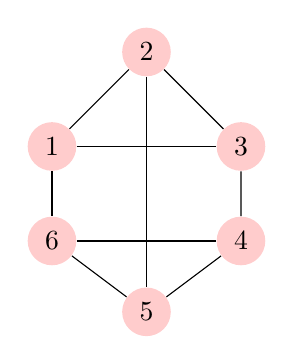
\begin{tikzpicture}
  [scale=.3,auto=left,every node/.style={circle,fill=red!20}]
  \node (n1) at (1,7) {1};
  \node (n2) at (5,11)  {2};
  \node (n3) at (9,7)  {3};
  \node (n4) at (9,3) {4};
  \node (n5) at (5,0)  {5};
  \node (n6) at (1,3) {6};
  
   \foreach \from/\to in {n1/n2,n2/n3,n3/n4,n4/n5,n5/n6,n1/n6,
  n2/n5, n6/n4,n1/n3}
    \draw (\from) -- (\to);
    \end{tikzpicture}
\caption{ A nonbipartite Graph with 6 vertices and 9 edges}\label{8g4}

\end{figure}

Ajur thought for a while and said that partial solutions to the isomorphism problem would be very useful when you want to test whether a given graph is in a collection of graphs, a problem that comes up in chemistry. Rishnak was pleased to notice that Ajur's was thinking about practical applications of graph theory. 

Ajur wanted to kmow if there is an easier method for testing isomorphism between rooted trees. Rishnak smiled and said there is a faster method for rooted trees. First, Rishnak explained a certain canonical representation for a labeled tree, called a Pr\"ufer code. The construction is iterative, and the Pr\"ufer code of a labeled tree with $n$ vertices is a code of length $n-2$. First, we recall that a leaf of a tree is a vertex that is connected to only one other vertex.

\begin{enumerate}
\item let Pr{\"u}fer code be an empty set,

\item Start with a leaf vertex of smallest label, say v. Find the vertex connecting it to the rest of tree say w.  Remove v from the tree and add w to the Pr{\"u}fer Code
 
\item Repeat the previous step until we are left with two vertices.
\end{enumerate}

We implement this procedure for the following tree, in Example \ref{8g5}. The smallest leaf vertex is 4. Its adjacent vertex is labeled 2. So 2 is added to the Pr{\"u}fer code and vertex 4 is removed. Next smallest vertex is 5 and its adjacent vertex is 2. Hence 2 is added to the Pr{\"u}fer code and vertex labeled 5 is removed. Now 2 is the smallest leaf vertex and its adjacent vertex is 1 and  1 is added to Pr{\"u}fer code and vertex 2 is removed. Currently Pr{\"u}fer code is \textbf{221}. Now 1 is the smallest labeled vertex and its adjacent vertex is 3 and vertex 1 is removed. Hence 3 is added to Pr{\"u}fer code which becomes \textbf{2213}. The next smallest leaf vertex is 6 and its adjacent vertex is 3. 3 is added to Pr{\"u}fer code. There are only two vertices left and we are done. The Pr{\"u}fer code for tree in Example \ref{8g5} is \textbf{22133}. From this Pr{\"u}fer code, one can conclude that there are 7 vertices in the tree (as the Pr{\"u}fer code is of length $n-2$ for a tree with $n$ vertices). Further, we can also conclude that vertices labeled 4,5,6 and 7 are leaf vertices as they do not appear in the given Pr{\'u}fer code. 
\begin{figure}
\begin{center}

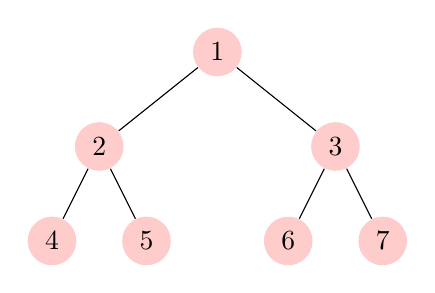
\begin{tikzpicture}
  [scale=.6,auto=left,every node/.style={circle,fill=red!20}]
  \node (n1) at (5.5,7) {1};
  \node (n2) at (3,5)  {2};
  \node (n3) at (8,5)  {3};
  \node (n4) at (2,3) {4};
  \node (n5) at (4,3)  {5};
  \node (n6) at (7,3)  {6};
  \node (n7) at (9,3)  {7};

  \foreach \from/\to in {n1/n2,n1/n3,n2/n4,n2/n5,n3/n6,n3/n7}
    \draw (\from) -- (\to);

\end{tikzpicture}

\caption{Tree with 7 vertices and four leaf vertices at the ground. }\label{8g5}
\end{center}
\end{figure}

Ajur then wanted to know if one could have a code for unlabeled trees. Rishnak replied with a resounding yes and explained the basic steps for a rooted tree. For any tree, one needs to choose an appropriate root vertex \footnote{Center of a tree is chosen as the root vertex \textbf{Raju: be careful, not every tree has a center which is a vertex!}} 
\begin{enumerate}
    \item  Label the leaf vertices as 01.
    \item Let $x$ be a non-leaf vertex. If all the children of $x$, sort these labels in alphabetical order. \footnote{0 comes before 1} The label of vertex $x$ is 0 followed by concatenation of the (sorted) labels of the children followed by 1.
    \item Stop after you label the root vertex.
\end{enumerate}

For example for the tree in \ref{8g5} leaf vertices 4,5,6,7 are all labeled \textbf{01}. Vertex 2 is labeled \textbf{001011} and vertex 3 has a similar label \textbf{001011}. Finally root vertex has the label \textbf{00101100101111}. This \textbf{00101100101111} becomes the code for the tree.

Rishnak continued that closely related to Graph Isomorphism is a problem that has plenty of uses in real life - and not just in the ghoulish realm. Ajur chuckled at the bad joke but politely retrained from interrupting. Rishank continued with the statement of the next problem.  Instead of asking whether two graphs are structurally similar, given two graphs $G$ and $H$, the subgraph isomorphism problem asks if there is a subgraph of $G$ that is isomorphic to H. Ajur responded immediately saying this approach can be used to test if a graph $G$ with $n$ vertices has a Hamiltonian cycle by choosing $H$ to be a cycle of length $n$ and asking whether there is a subgraph of $G$ isomorphic to $H$. Rishnak nodded in agreement and said that is the reason the subgraph Isomorphism problem is hard. On the other hand, if both $G$ and $H$ are labeled graphs, there are heuristics to test whether $H$ occurs in $G$ as a subgraph. This type of labeled subgraph isomorphism problem has many applications in medical imaging and chemical structure identifications.


\chapter{Planar Graphs}
Ajur was so enamored by Hamiltonian cycles, he was eager to meet Rishnak and hear more about them. Rishnak wanted to introduce a different concept: drawing graphs.
A planar drawing of a graph is one in which no edges cross each other (except at
the vertices). By definition, a \emph{planar graph} is a graph for which there exists at least one planar drawing.
If a graph does not admit any planar drawings, we call it a \emph{non-planar graph}.
For example here are two drawings of a complete graph on four vertices $K_4$. Since Figure \ref{9g2} has no edges crossing, we can call $K_4$ a planar graph.
\begin{figure}
\begin{center}
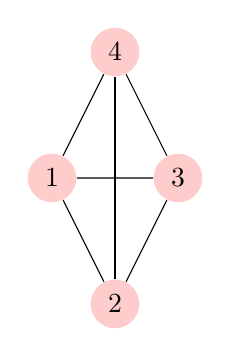
\begin{tikzpicture}
  [scale=.4,auto=left,every node/.style={circle,fill=red!20}]
  \node (n1) at (1,7) {1};
  \node (n2) at (3,3)  {2};
  \node (n3) at (5,7)  {3};
  \node (n4) at (3,11)  {4};

  \foreach \from/\to in {n1/n2,n2/n3,n2/n4,n1/n4,n3/n4,n1/n3} 
  \draw (\from) -- (\to);

\end{tikzpicture}
\caption{ Drawing of $K_4$ in which edges cross}\label{9g1}
\end{center}
\end{figure}
\begin{figure}
\begin{center}
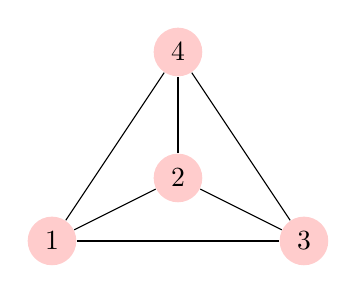
\begin{tikzpicture}
  [scale=.4,auto=left,every node/.style={circle,fill=red!20}]
  \node (n1) at (-1,7) {1};
  \node (n2) at (3,9)  {2};
  \node (n3) at (7,7)  {3};
  \node (n4) at (3,13)  {4};

  \foreach \from/\to in {n1/n2,n2/n3,n2/n4,n1/n4,n3/n4,n1/n3}
    \draw (\from) -- (\to);

\end{tikzpicture}
\caption{ Planar drawing of $K_4$}\label{9g2}
\end{center}
\end{figure}
 Rishnak asked Ajur whether he could draw the graph in Figure \ref{9g3} with no edges crossing.
 \begin{figure}
\begin{center}
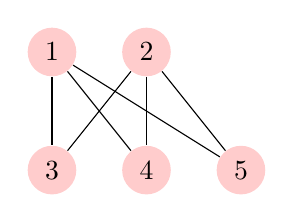
\begin{tikzpicture}
  [scale=.3,auto=left,every node/.style={circle,fill=red!20}]
  \node (n1) at (1,7) {1};
  \node (n2) at (5,7)  {2};
  \node (n3) at (1,2)  {3};
  \node (n4) at (5,2) {4};
  \node (n5) at (9,2)  {5};
 
  
   \foreach \from/\to in {n1/n3,n1/n4,n1/n5,n2/n3,n2/n4,n2/n5}
    \draw (\from) -- (\to);
    \end{tikzpicture}
\caption{ A bipartite graph with 5 vertices and 6 edges, denoted by $K_{2,3}$, where the edges cross}\label{9g3}
\end{center}
\end{figure}
Ajur thought for a while and found it a bit challenging. Then he thought of moving the vertex 2 down in which case no edges will cross. He drew the graph as shown in Figure \ref{9g4}
\begin{figure}
\begin{center}
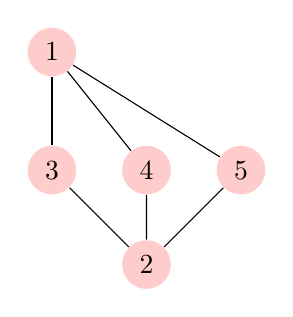
\begin{tikzpicture}
  [scale=.3,auto=left,every node/.style={circle,fill=red!20}]
  \node (n1) at (1,7) {1};
  \node (n2) at (5,-2)  {2};
  \node (n3) at (1,2)  {3};
  \node (n4) at (5,2) {4};
  \node (n5) at (9,2)  {5};
 
  
   \foreach \from/\to in {n1/n3,n1/n4,n1/n5,n2/n3,n2/n4,n2/n5}
    \draw (\from) -- (\to);
    \end{tikzpicture}
\caption{ Planar drawing of a bipartite graph $K_{2,3}$ with 5 vertices and 6 edges, with no edge crossings}\label{9g4}
\end{center}
\end{figure}

Impressed, Rishnak then asked Ajur whether the graph in Figure \ref{9g5} has a planar representation. Ajur struggled and tried to get a planar drawing --- but ended up with one edge crossing, see Figure \ref{9g6}. 

\begin{figure}
\begin{center}
\begin{tikzpicture}
  [scale=.3,auto=left,every node/.style={circle,fill=red!20}]
  \node (n1) at (1,7) {1};
  \node (n2) at (5,7)  {2};
  \node (n3) at (9,7) {3};
  \node (n4) at (1,2)  {4};
  \node (n5) at (5,2) {5};
  \node (n6) at (9,2)  {6};
 
  
   \foreach \from/\to in {n1/n6,n1/n4,n1/n5,n2/n6,n2/n4,n2/n5,n3/n4,n3/n5,n3/n6}
    \draw (\from) -- (\to);
    \end{tikzpicture}
\caption{ A bipartite graph with 6 vertices and 9 edges, denoted by $K_{3,3}$, where the edges cross}\label{9g5}
\end{center}
\end{figure}
\begin{figure}
\begin{center}
\begin{tikzpicture}
  [scale=.4,auto=left,every node/.style={circle,fill=red!10}]
  \node (n1) at (1,7) {1};
  \node (n2) at (5,-2)  {2};
  \node (n3) at (7,3) {3};
  \node (n4) at (1,2)  {4};
  \node (n5) at (4,1) {5};
  \node (n6) at (11,3)  {6};
 
  
   \foreach \from/\to in {n1/n6,n1/n4,n1/n5,n2/n6,n2/n4,n2/n5,n3/n4,n3/n5,n3/n6}
    \draw (\from) -- (\to);
    \end{tikzpicture}
\caption{ A  drawing of a bipartite graph with 6 vertices and 9 edges, denoted by $K_{3,3}$, where just two edges edges cross}\label{9g6}
\end{center}
\end{figure}
Rishnak then told Ajur that this graph does not have a planar representation. He added that there is a well-known related puzzle credited to Sam Loyd\footnote{Sam Loyd is a famous American recreational mathematician and puzzler.}. There are three houses (represented as circles) drawn on paper and below them three smaller circles representing gas, water, and electricity suppliers. The aim of the puzzle is to draw lines to get each utility into every house, without crossing over any line. Ajur reminded himself that he should read up on Loyd's puzzle books from his local library.

 Rishnak asked Ajur if two graphs $G$ and $H$ are isomorphic and if $G$ is planar, can you say $H$ is planar. Ajur said if $H$ is isomorphic to $G$, then each vertex corresponds to some vertex of $G$. By just relabeling the vertices of $G$ in its planar drawing, we get a planar drawing of $H$.
 
 Ajur then excitedly told Risnak that all trees have a planar representation\footnote{Ajur liked monkeys and monkeys liked trees. It followed by transitivity that Ajur liked trees.}. Rishnak answered that trees are indeed easy to embed in a plane as there are
 no cycles. He added that there are interesting space-filling planar representations of trees, for example in Figure \ref{9g7}.
\begin{figure}
\begin{center}    

 \begin{tikzpicture}[decoration=H-tree, very thick]
    \draw decorate { decorate { decorate { decorate { decorate { decorate { (0,0) -- (3,0) }}}}}};
  \end{tikzpicture}
  \caption{ A planar drawing of a tree (which is self similar)}\label{9g7}
  \end{center}
\end{figure}

One way to get a planar drawing is to embed the longest cycle in a plane and then try to place the rest of the vertices so that no edges cross each other. This cycle will divide the plane into two regions --- the inner region (inside the cycle) and the outer region (outside the cycle). So the edges have to go either inside or outside. By trying out the possibilities, you can get a planar representation of a graph (if one exists). Of course, this process is easier said than done. There is in fact an efficient method of placing the edges, without any backtracking, but Rishnak added that details are rather complicated. 

Each region in a planar representation is also referred to as a face. Euler discovered a remarkable formula concerning the number of edges, $e$, the number of vertices, $n$, and the number of faces, $f$ of a planar graph:
\begin{equation}
\label{eqn:euler}
  f-e+n=2 
\end{equation}

 

Rishnak proceeded to give an intuitive explanation of this formula \ref{eqn:euler}. Each region corresponds to a cycle and the external region (sometimes called an infinite region) also comes from a cycle. 
There are $n-1$ edges in a tree, and the rest of the $e-(n-1)$ edges in a graph will form part of a cycle. We will show in chapter 11. a spanning tree in a connected graph and how to choose one.
%\textbf{You implicitly pick a spanning tree, which you have not yet discussed! Consider saying: it turns out, as we'll learn in Chapter ***, that there exists a ``maximal tree" of any graph.} 
Each of these cycles correspond to an internal region or internal face, and there is one external face. From this, Euler's equation \ref{eqn:euler} follows.
\begin{eqnarray}
    \label{eqn:cycles}
    \text{internal faces}&=&e-(n-1)\nonumber\\
    \text{external face}&=&1 \nonumber \\
    \text{total faces}&=& \text{internal faces}~+~\text{external face} \nonumber \\
    &=&e-n+2
\end{eqnarray}

Ajur said that he has constructed Platonic solids with Zometools\footnote{Zometool is a commercial kit to make general polyhedra.}. Rishnak then explained Euler's equation applied for the five platonic solids; the graph theory in Euler's formula can be used to relate vertices, edges, and faces of the platonic solids! See Table \ref{tab:platonic} where $n$ stands for the number of vertices, $e$ stands for the number of edges and $f$ stands for the number of faces. All Platonic solids have a planar representation as shown in Figures \ref{fig:tetra}, \ref{fig:octa}, \ref{fig:cube}, \ref{fig:dod}, and \ref{fig:ico}\footnote{The reason is that every platonic solid embeds in sphere, and can be chosen such that no point or vertex passes the North pole. Then one may stereographically project the graph to the plane.}.
\begin{table}[ht]
    \centering
    \begin{tabular}{||c|c|c|c||}
    \hline
    Solid & n & e& f \\ [0.5ex] 
 \hline\hline
 Tetrahedron& 4 & 6 & 4 \\ 
 \hline
 Octohedron & 6 & 12& 8 \\
 \hline
 Cube & 8 & 12 & 6 \\
 \hline
 Dodecahedron & 20 & 30 & 12 \\
 \hline
 Icosahedron & 12 & 30 & 20 \\ [1ex] 
 \hline
 \end{tabular}
    \caption{Euler Equation for Platonic Solids}
    \label{tab:platonic}
\end{table}
\begin{figure}

  
\begin{tikzpicture}
[scale=0.7]
        \grTetrahedral
    \end{tikzpicture}
\caption{tetrahedron}
\label{fig:tetra}
\end{figure}
\begin{figure}
    \begin{tikzpicture}

        \grOctahedral[RA=5,RB=1]
    \end{tikzpicture}
\caption{Octahedron}\label{fig:octa}
\end{figure}
\begin{figure}
    \begin{tikzpicture}

        \grCubicalGraph
    \end{tikzpicture}
\caption{Cube}\label{fig:cube}
\end{figure}
\begin{figure}
    \begin{tikzpicture}
    [scale=0.8]

        \grDodecahedral[form=2] 
    \end{tikzpicture}
    \caption{Dodecahedron}\label{fig:dod}
\end{figure}
\begin{figure}
    \begin{tikzpicture}

        \grIcosahedral[form=2,RA=8]
    \end{tikzpicture}
\caption{Icosahedron}\label{fig:ico}
\end{figure}

Rishnak said each edge appears in exactly two faces. If each face is a triangle (cycle of length 3), it is called a maximal planar graph. Hence we deduce $e=\frac{3 \times f}{2}$ or $f=\frac{2 \times e}{3}$ . Substituting for $f$ in Euler's equation \ref{eqn:euler}, we get

\begin{eqnarray}
  \label{eqn:maxplanar}  
    \frac{2\times e}{3}&=&e-n+2\nonumber\\
    -\frac{e}{3} &=&-n+2\nonumber \\
    \frac{e}{3}&=&n-2 \nonumber \\
    e&=& 3 \times n - 6
\end{eqnarray}

Using Equation \ref{eqn:maxplanar}, it can be shown that the complete graph on 5 vertices, $K_5$ shown in Figure \ref{9g10}, is nonplanar. That graph has $n$=5, $e$=10. If it were planar then the number of edges would have to be at most $9$. 
Rishnak asked Ajur: can you use Euler's equation to show that $K_{3,3}$, a complete bipartite graph on 6 vertices (discussed in Figure \ref{9g5}), is nonplanar? 
Ajur was alert and he knew that the bipartite graph has only even cycle lengths. To have the maximum number of edges each face has to be of a cycle length 4. Hence $2\times e =4 \times f$ or $f=\frac{e}{2}$. Substituting for $f$ in Euler's equation \ref{eqn:euler}
$f=e-n+2$, one gets $-\frac{e}{2}=n-2$ or $e=2\times n -4$. Substituting for $n=6$, we get $e=8$. That is the maximum number possible. However, $K_{3,3}$ has 9 edges which is more than 8. Hence Ajur had proven that $K_{3,3}$ is nonplanar.
\begin{figure}
\begin{center}
\begin{tikzpicture}
  [scale=.5,auto=left,every node/.style={circle,fill=red!20}]
  \node (n1) at (1,7) {1};
  \node (n2) at (5,11)  {2};
  \node (n3) at (9,7)  {3};
  \node (n4) at (9,3) {4};
  \node (n5) at (1,3) {5};

  \foreach \from/\to in {n1/n2,n2/n3,n3/n4,n4/n5,n1/n5,n1/n3,n1/n4,n2/n4,n2/n5,n3/n5}
    \draw (\from) -- (\to);

\end{tikzpicture}
\caption{ Complete Graph, $K_5$ with 5 vertices and 10 edges }\label{9g10}
\end{center}
\end{figure}
Rishnak added another interesting fact (without adding any further details) that any planar graph has not only a plane representation but also a representation in which each edge is drawn as a straight line.

Ajur responded that every subraph of a planar graph is also a planar graph. Pleased to note that Ajur was following the concepts, Rishnak added that the operation of dividing an edge, i.e., introducing vertices of degree 2 will not change the embedding. If a graph is planar and if we subdivide an edge, it is still planar. Similarly if a graph is nonplanar, and if e subdivides any edge, the graph is still nonplanar. An example of subdivision of an edge is shown in Figure \ref{9g9}. Now Jura appeared to be getting restless and Rishnak decided that they had had enough for that session, so they parted for the night.

\begin{figure}[h]
\begin{center}
\begin{tikzpicture}
  [scale=.8,auto=left,every node/.style={circle,fill=red!20}]
  \node (n1) at (-1,7) {1};
  \node (n2) at (3,9)  {2};
  \node (n3) at (7,7)  {3};
  \node (n4) at (3,13)  {4};
  \node (n5) at (2,7) {5};
  \node (n6) at (4,7) {6};
 \foreach \from/\to in {n1/n2,n2/n3,n2/n4,n1/n4,n3/n4,n1/n5,n5/n6,n6/n3}
    \draw (\from) -- (\to);
\end{tikzpicture}
\caption{ Subdivision of edge (1,3) by adding two new vertices 5 and 6 in Figure \ref{9g2}}\label{9g9}
\end{center}
\end{figure}

\textbf{Question for the seventh day:} Rishnak asked Ajur to show that there exists at least one vertex of degree 5.
\textbf{Answer:} Ajur remembered Euler equation \ref{eqn:euler}. He said that each edge occurs exactly in two faces. The smallest face could be a cycle of length 3. Hence, substituting for $f=\frac{2 \times e}{3}$ in  
$\frac{2 \times e} {3} =e-n+2$, resulting in $\frac{e}{3}=n-2$ or $e=3\times n -6$. Thus $3 \times n-6$ is the maximum number of edges a planar graph can have (he derived Equation \ref{eqn:maxplanar} once again). Ajur reasoned that if all vertices have degree 6 or more, then $e~\ge~ 3 \times n$, contradicting that the graph is planar.

Rishnak was happy with Ajur's answer and they adjourned for the day.


\chapter{Coloring}
Rishnak was eager to meet Ajur, as he was impressed with his logical reasoning. Finally he found Ajur walking along with Jura. Rishnak caught up with Ajur. Rishnak asked Ajur whether Ajur likes coloring. Ajur responded that he really enjoyed coloring and it had a calming effect on him.

Rishnak was glad to hear that. He said that there is also a way to color the vertices of a graph. Rishnak added that a proper vertex coloring is coloring of vertices such that no adjacent vertices (i.e., vertices connected by an edge) can get the same color. To make it more interesting the question is what is the smallest number of colors to properly vertex color a graph. 
Rishnak showed an example of proper coloring of a graph \ref{10g1} with 4 colors. Ajur jumped up and down and said that he could color it three colors and showed his coloring in \ref{10g2}.
\begin{figure}[h]
\begin{center}
\begin{tikzpicture}
  [scale=.8,auto=left,every node/.style={circle}]
  \node (n1)[fill=blue] at (-1,7) {1};
  \node (n2)[fill=green] at (3,9)  {2};
  \node (n3)[fill=red] at (7,7)  {3};
  \node (n4)[fill=yellow] at (3,13)  {4};
  \node (n5)[fill=red] at (2,7) {5};
  \node (n6)[fill=blue] at (4,7) {6};
 \foreach \from/\to in {n1/n2,n2/n3,n2/n4,n1/n4,n3/n4,n1/n5,n5/n6,n6/n3}
    \draw (\from) -- (\to);
\end{tikzpicture}
\caption{ Proper Coloring the vertices of a graph with 4 colors}\label{10g1}
\end{center}
\end{figure}

\begin{figure}[h]
\begin{center}
\begin{tikzpicture}
  [scale=.8,auto=left,every node/.style={circle}]
  \node (n1)[fill=blue] at (-1,7) {1};
  \node (n2)[fill=green] at (3,9)  {2};
  \node (n3)[fill=blue] at (7,7)  {3};
  \node (n4)[fill=yellow] at (3,13)  {4};
  \node (n5)[fill=red] at (2,7) {5};
  \node (n6)[fill=yellow] at (4,7) {6};
 \foreach \from/\to in {n1/n2,n2/n3,n2/n4,n1/n4,n3/n4,n1/n5,n5/n6,n6/n3}
    \draw (\from) -- (\to);
\end{tikzpicture}
\caption{ Proper Coloring the vertices of a graph with 3 colors colors}\label{10g2}
\end{center}
\end{figure}

Ajur further stated that 3 colors are needed a vertices 1, 2 and 4 are mutually adjacent and those vertices need 3 different colors. 
Rishnak asked Ajur to properly color the graph $K_{3,3}$, a complete bipartite graph. Ajur jumped at the opportunity and showed a 2 coloring of this graph \ref{10g3}
\begin{figure}
\begin{center}
\begin{tikzpicture}
  [scale=.4,auto=left,every node/.style={circle}]
  \node (n1)[fill=red] at (1,7) {1};
  \node (n2)[fill=red] at (5,7)  {2};
  \node (n3)[fill=red] at (9,7) {3};
  \node (n4) [fill=blue] at (1,2)  {4};
  \node (n5) [fill=blue] at (5,2) {5};
  \node (n6)[fill=blue] at (9,2)  {6};
 
  
   \foreach \from/\to in {n1/n6,n1/n4,n1/n5,n2/n6,n2/n4,n2/n5,n3/n4,n3/n5,n3/n6}
    \draw (\from) -- (\to);
    \end{tikzpicture}
\caption{ Two coloring of a Bipartite Graph with 6 vertices and 9 edges, denoted by $K_{3,3}$}\label{10g3}
\end{center}
\end{figure}

Ajur further said that any bipartite graph Vertices are partitioned into two sets $A$ and $B$ and the edges always go from one set, $A$, to the other set, $B$. Ajur further stated that all the vertices in $A$ can be colored with one color, say, red and all the vertices in $B$ can be colored with another color, say blue. Since all tress are also bipartite graphs (contains cycles of even length (=0)), trees can be colored with just two colors. He showed an example \ref{10g4}. Coloring of trees reminded Ajur of the beautiful fall colors one sees in the trees!
\begin{figure}
\begin{center}

\begin{tikzpicture}
  [scale=.6,auto=left,every node/.style={circle}]
  \node (n1)[fill=red] at (5.5,7) {1};
  \node (n2)[fill=blue] at (3,5)  {2};
  \node (n3)[fill=blue] at (8,5)  {3};
  \node (n4)[fill=red] at (2,3) {4};
  \node (n5)[fill=red] at (10,3)  {5};


  \foreach \from/\to in {n1/n2,n1/n3,n2/n4,n3/n5}
    \draw (\from) -- (\to);

\end{tikzpicture}

\caption{Two coloring of a tree }\label{10g4}
\end{center}
\end{figure}

Map Coloring problem is to color the regions or faces of a planar graph (maps are usually drawn on a plane) so that no two adjacent faces or regions are colored the same.





\chapter{Spanning Trees and How to find them}
Rishnak found Ajur and Jura walking along a stretch of road with trees on either side. Recalling his previous talks with Ajur about trees, Rishnak chose a specific kind of tree in a graph for his next session with Ajur.
In a connected graph $G=(V,E)$ (connected means that there is a path between every pair of vertices in $G$), a tree (spanning all the vertices) is a subgraph =$T(V,E_1)$ of G satisfying the two conditions:
\begin{enumerate}
    \item The subgraph, T,  is a tree. (i.e., contains no cycles and of course connected; i.e., there is only one path between every pair of vertices.)
    \item Vertex set of $T$ is the same as the vertex set of $G$.
\end{enumerate}

Here is an example of Graph Figure \ref{11g1} and a subgraph of this graph which is a spanning tree shown in Figure \ref{11g2} 
\begin{figure}
\begin{center}
\begin{tikzpicture}
  [scale=.6,auto=left,every node/.style={circle,fill=red!20}]
  \node (n6) at (1,10) {6};
  \node (n4) at (4,8)  {4};
  \node (n5) at (8,9)  {5};
  \node (n1) at (11,8) {1};
  \node (n2) at (9,6)  {2};
  \node (n3) at (5,5)  {3};

  \foreach \from/\to in {n6/n4,n4/n5,n5/n1,n1/n2,n2/n5,n2/n3,n3/n4}
    \draw (\from) -- (\to);

\end{tikzpicture}
\caption{ Example Graph with 6 vertices and 7 edges}\label{11g1}
\end{center}
\end{figure}
\begin{figure}
\begin{center}
\begin{tikzpicture}
  [scale=.6,auto=left,every node/.style={circle,fill=red!20}]
  \node (n6) at (1,10) {6};
  \node (n4) at (4,8)  {4};
  \node (n5) at (8,9)  {5};
  \node (n1) at (11,8) {1};
  \node (n2) at (9,6)  {2};
  \node (n3) at (5,5)  {3};

  \foreach \from/\to in {n6/n4,n4/n5,n5/n1,n1/n2,n3/n4}
    \draw (\from) -- (\to);

\end{tikzpicture}
\caption{ Subgraph of \ref{11g1} which is a spanning tree of \ref{11g1} - Spanning tree has 6 vertices and 5 edges}\label{11g2}
\end{center}
\end{figure}
Rishnak asked Ajur if he can construct one more spanning tree for this graph \ref{11g1}. Ajur was eager to show off and drew the following graph \ref{11g3}.
\begin{figure}
\begin{center}
\begin{tikzpicture}
  [scale=.6,auto=left,every node/.style={circle,fill=red!20}]
  \node (n6) at (1,10) {6};
  \node (n4) at (4,8)  {4};
  \node (n5) at (8,9)  {5};
  \node (n1) at (11,8) {1};
  \node (n2) at (9,6)  {2};
  \node (n3) at (5,5)  {3};

  \foreach \from/\to in {n6/n4,n4/n5,n5/n1,n2/n5,n3/n4}
    \draw (\from) -- (\to);

\end{tikzpicture}
\caption{ Another Spanning Tree of Graph in \ref{11g1}}\label{11g3}
\end{center}
\end{figure}

Rishnak then asked Ajur how many distinct spanning trees (labelled non isomorphic) there are. Ajur had a quick answer this time too. There are two cycles in this graph, namely (2,3,4,5) and (1,5,2). One is of 
length 4 and the other is of length 3. But they share a common edge (2,5). There are 4 possible spanning trees to choose from the cycle of length 4 and there are 3 possibilities to choose from the other cycle - giving rise to 12 possibilities. But one of them contains a cycle (if (edge (5,2) omitted in the 4 cycle and in the 3 cycle); thus giving rise to 11  spanning trees. They are enumerated.   
The edge (4,6) has to be present in every spanning tree. The eleven spanning tree edges are given below.
\begin{enumerate}
    \item \{(4,6),(4,5),(5,2),(2,3),(5,1)\}
    \item \{(4,6),(4,5),(5,2),(2,3),(2,1)\}
    \item \{(4,6),(4,5),(4,3),(5,2),(5,1)\}
    \item \{(4,6),(4,5),(4,3),(5,2),(2,1)\}
    \item \{(4,6),(4,3),(2,3),(5,2),(5,1)\}
    \item \{(4,6),(4,3),(2,3),(5,2),(2,1)\}
    \item \{(4,6),(4,5),(4,3),(2,3),(5,1)\}
    \item \{(4,6),(4,5),(4,3),(2,3),(2,1)\}
    \item \{(4,6),(4,5),(2,3),(5,1),(1,2)\}
    \item \{(4,6),(4,5),(4,3),(5,1),(1,2)\}
    \item \{(4,6),(4,3),(3,2),(2,1),(1,5)\}
\end{enumerate}

Ajur asked what the maximum number of labeled spanning trees i is n a graph with $n$ vertices. Ajur added that the maximum number of spanning trees will be present in a complete graph as it has the maximum number of edges in a $n$ vertex graph. Rishnak agreed that complete graphs have the largest number of spanning trees. We can find the number of spanning trees in a complete graph using Pr{\"u}fer code (which we talked about a couple of days ago) in Chapter 8. Ajur remembered it and interjected for a $n$ vertex tree, one needed only a Pr{\"u}fer code of length $n-2$. Rishnak agreed and said that the Pr{\"u}fer code is of length $n-2$ for a $n$ vertex graph. Each of the $n-2$ characters in a code to be any of the $n$ vertices. Hence the number of (labeled) spanning trees in a complete graph with $n$ vertices is $n^{n-2}$.

Since there are $n-1$ edges in a spanning tree, each of the remaining $e-n+1$ edges when taken with a spanning tree will create a cycle. Thus there will be $e-n+1$ cycles. These cycles are called Fundamental cycles. Each fundamental cycle has exactly one non spanning tree edge.\footnote{Euler's equation \ref{eqn:euler} in chapter 9 uses this fact.} Rishnak showed with an example Figure \ref{11g4}.

\begin{figure}
\begin{center}
\begin{tikzpicture}
  [scale=.6,auto=left,every node/.style={circle,fill=red!20}]
  \node (n6) at (1,10) {6};
  \node (n4) at (4,8)  {4};
  \node (n5) at (8,9)  {5};
  \node (n1) at (11,8) {1};
  \node (n2) at (9,6)  {2};
  \node (n3) at (5,5)  {3};

  \foreach \from/\to in {n6/n4,n4/n5,n5/n1,n1/n2,n3/n4}
    \draw [thick] (\from) -- (\to);
  \foreach \from/\to in {n5/n2,n2/n3}
   \draw [color=red] (\from) -- (\to);
\end{tikzpicture}
\caption{ Two fundamental cycles of \ref{11g1} with respect to a spanning tree of \ref{11g2} - Spanning tree edges are shown as thick lines and non-spanning tree edges are shown in red color. Fundamental Cycles are (1,2,5) and (4,5,1,2,3)}\label{11g4}
\end{center}
\end{figure}

Ajur asked Rishnak how to find a spanning tree for a given graph. Rishnak said that the graph has to be connected.\footnote{Between every pair of vertices there is a path.} It can be done using the following steps.
\begin{figure} 
\begin{enumerate}
\item Start from any vertex. Include that vertex in a bag.
\item From the vertices in a bag, find a vertex,$v$, (not in a bag) that is adjacent to one of the vertices,$w$, in the bag. Include that edge, $(v,w)$ in the spanning tree.
\item Repeat the above step till all the vertices are in the bag.
\end{enumerate}
\caption{Finding a Spanning Tree Procedure}\label{11a1}
\end{figure}
Rishnak illustrated his procedure for the example in Figure \ref{11g1}.
Put vertex labeled 1 in the bag. Its adjacent vertices are labeled 2 and 5. Choose vertex (the choice is arbitrary) labeled 5 and put in the bag. Edge (1,5) is included in the spanning tree. From vertices in the bag find a vertex that is adjacent (but not in the bag). Choices are either vertices labeled 2 or 4. Choose the vertex labeled 2 and include edge (1,2) in the spanning tree (We could have also included (5,2) instead of (1,2) in the spanning tree.). Now the bag contains the vertices (1, 2, 5). Find a vertex that is adjacent to any of these vertices (that are not in the bag). They are namely vertices labeled 4 and 3. Choose (this choice is arbitrary) the vertex labeled 4 and include the edge (4,5) in the spanning tree. Now vertices (1,2,4,5) are in the bag. From these vertices find a vertex that is adjacent but not in the bag. They will be 6 and 3.  Choose the vertex labeled 3 and include the edge (4,3) in the spanning tree. The bag contains the vertices (1,2,3,4,5). The vertex that is adjacent to one
of the vertices in the bag is labeled 6. Choose that vertex labeled 6 and include the edge (4,6) in the spanning tree. Now the bag contains all the vertices and we have the spanning tree edges (1,5), (1,2), (5,4), (4,3) and (4,6). This is the same spanning tree shown in Figure \ref{11g2}.

If we had made different choices, we will get a different spanning tree as shown in Figure \ref{11g3}.

A graph is weighted if there are weights associated with an edge. The weight could represent the distance in miles or the cost of travel etc. Here is an example of a weighted graph with the weighted edges.
\begin{figure}
\begin{center}
\begin{tikzpicture}
  [scale=.6,auto=left,every node/.style={circle,fill=red!20}]
  \tikzstyle{weight} = [draw=blue!15,shape=rectangle]
  \node (n6) at (1,10) {6};
  \node (n4) at (4,8)  {4};
  \node (n5) at (8,9)  {5};
  \node (n1) at (11,8) {1};
  \node (n2) at (9,6)  {2};
  \node (n3) at (5,5)  {3};
  \foreach \source /\dest /\weight in {n6/n4/1,n4/n5/2,n5/n1/5,n1/n2/2,n2/n5/3,n2/n3/8,n3/n4/7} 
   \draw (\source) --node[weight] {$\weight$}  (\dest);
\foreach \source /\dest /\weight in {1/3/1} place \weight above of=\path;
  
  \end{tikzpicture}
\caption{ Example weighted Graph with 6 vertices and 7 edges - weights are associated with edges}\label{11g7}
\end{center}
\end{figure}

Rishnak then told Ajur of an interesting problems - to find a minimum spanning tree in a weighted graph. In other words find a spanning tree where the sum of all the edge weights(in a spanning tree) is the smallest. Ajur responded saying one can enumerate all spanning trees and compute for each spanning tree the sum of weights and choose the spanning tree with the smallest edge weight sum. Rishnak smiled on hearing  "Brute Force" method - a good strategy that can work for most problems. The problem is to find if there more efficient method\footnote{Informally a faster method that makes choices so that one does not have to consider at all spanning trees. Usually these run quickly in a computer.} We can adapt/modify the procedure/method described in Figure \ref{11a1} as follows.
\begin{figure} 
\begin{enumerate}
\item Start from any vertex. Include that vertex in a bag.
\item From the vertices in a bag, find a vertex , $v$, (not in a bag) that is adjacent to one of the vertices,$w$, in the bag and with the smallest edge weight $(v,w)$. Include that edge in the minimum spanning tree.
\item Repeat the above step till all the vertices are in the bag.
\end{enumerate}
\caption{Finding a  Minimum Spanning Tree Procedure}\label{11aa}
\end{figure}

Ajur chose to work through the example shown in Figure \ref{11g7}. He choose vertex labeled 1 in the bag. Then the vertex labeled 2 is put in the bag as the edge weight (1,2) is the smallest from veretx labeled 1. Now vertices labeled 1 and 2 are in the bag. Edge (2,5) is the smallest edge weight and hence (2,5) is included in the minimum spanning tree and vertex labeled 5 is put in the bag. Among vertices in the bag, namely 1, 2 and 5, the edge (5,4) has the smallest weight. Now the bag contains vertices labeled 1,2,5 and 4. The edge (4,6) is the smallest weight. Hence vertex labeled 6 is included in the bag and edge (4,6) is added to the minimum spanning tree. Edge (4,7) is the smallest weight and hence edge (4,7) is  included in the minimum spanning tree. Now the bag contains all the vertices and hence Ajur exclaimed that he found the minimum spanning tree.
Ajur drew the minimum spanning tree in the following Figure \ref{11g8}

\begin{figure}
\begin{center}
\begin{tikzpicture}
  [scale=.6,auto=left,every node/.style={circle,fill=red!20}]
  \tikzstyle{weight} = [draw=blue!15,shape=rectangle]
  \node (n6) at (1,10) {6};
  \node (n4) at (4,8)  {4};
  \node (n5) at (8,9)  {5};
  \node (n1) at (11,8) {1};
  \node (n2) at (9,6)  {2};
  \node (n3) at (5,5)  {3};
  \foreach \source /\dest /\weight in {n6/n4/1,n4/n5/2,n1/n2/2,n2/n5/3,n3/n4/7} 
   \draw[thick] (\source) --node[weight] {$\weight$}  (\dest);
\foreach \source /\dest /\weight in {1/3/1} place \weight above of=\path;
  
  \end{tikzpicture}
\caption{ Minimum spanning Tree of the weighted Graph\ref{11g7}}\label{11g8}
\end{center}
\end{figure}

Ajur could not control his enthusiasm and exclaimed that he could use this procedure to minimally connect a given set of points in a plane. The distance between these points could be the length of straight lines joining them. Ajur showed his work Figure \ref{11g9}

\begin{figure}
\begin{center}
\begin{tikzpicture}
  [scale=1,auto=left,every node/.style={circle,fill=red!20}]
  \tikzstyle{weight} = [draw=blue!5,shape=rectangle]
  \node (n1) at (1,9)  {1};
  \node (n2) at (5,9) {2};
  \node (n3) at (5,5)  {3};
  \node (n4) at (1,5)  {4};
  \foreach \source /\dest /\weight in {n1/n2/4,n2/n3/4,n3/n4/4} 
   \draw[thick] (\source) --node[weight] {$\weight$}  (\dest);
\foreach \source /\dest /\weight in {1/3/1} place \weight above of=\path;
  \foreach \source /\dest /\weight in {n1/n4/4,n1/n3/5.6,n2/n4/5.6} 
   \draw[color=blue,thick,dotted] (\source) --node[weight] {$\weight$}  (\dest);
\foreach \source /\dest /\weight in {1/3/1} place \weight below of=\path;
  \end{tikzpicture}
\caption{ Minimum spanning Tree of a set of four points- Non minimum spanning tree edges are drawn as dotted lines}\label{11g9}
\end{center}
\end{figure}

Urpur, another ghost had been eavesdropping on all these conversations. Urpur wanted to show of that he is smarter than both Rishnak and Ajur, so started talking about the spanning tree called Steiner Tree, wherein one is allowed to add Steiner points/vertices that were not present in the original given set of vertices. With a clever addition of Steiner points, one can get a spanning tree which is smaller than the one Ajur found in \ref{11g9}. Urpur then showed the following Figure \ref{11g10}

\begin{figure}
\begin{center}
\begin{tikzpicture}
  [scale=1,auto=left,every node/.style={circle,fill=red!20}]
  \tikzstyle{weight} = [draw=blue!5,shape=rectangle]
  \node (n1) at (1,9)  {1};
  \node (n2) at (5,9) {2};
  \node (n3) at (5,5)  {3};
  \node (n4) at (1,5)  {4};
  \node (n5) at (2,7) {5};
  \node (n6) at (4,7) {6};
  \foreach \source /\dest /\weight in {n1/n5/2.23,n5/n6/2,n6/n2/2.23,n6/n3/2.23,n5/n4/2.23} 
   \draw[thick] (\source) --node[weight] {$\weight$}  (\dest);
\foreach \source /\dest /\weight in {1/3/1} place \weight below of=\path;
 
  \end{tikzpicture}
\caption{ Minimum Steiner Tree of a set of four points- Steiner points/vertices are 5 and 6}\label{11g10}
\end{center}
\end{figure}

Rishnak was very impressed with Urpur's thinking. Sensing that Ajur was feeling jealous that Urpur was grabbing his attention,

\textbf{Question for the ninth day}
Rishnak asked Ajur the following question: Consider a complete graph with with 8 vertices and 28 edges. 14 of the edges have weight
1 and 14 of the edges have weight 10. Which of the edges have which weights to answer the
following  two questions: 
\begin{enumerate}
    \item Show how to assign weights to the edges so as to achieve the smallest possible weight minimum weight spanning tree. What is the smallest weight?
\item Show how to assign weights to the edges so as to achieve the \textbf{largest} possible weight \textbf{minimum weight} spanning tree. What is the largest weight of the minimum spanning tree.
 
\end{enumerate}

\textbf{Answer:} Ajur could do the first part easily if there is a cycle of length 8, with edge weight being 1, the minimum spanning tree cost will be 7.

Ajur thought the second problem is a bit more challenging. To get the maximum weight, all edges incident on a vertex have to be of weight 10. That is possible with only two vertices. Hence the maximum weight the minimum spanning tree can have will be 25.


 Rishnak called it a night. Jura was happy now to get Ajur's attention and jumping with joy, left with Ajur.
\chapter{Shortest Paths}
Ajur had found a map of the cemetery. He used it to try to find the best way to go to the water fountain. Then he remembered his recent discussions with Rishnak and excitedly told Jura that by using graph theory methods, they would be able to find a path and maybe even the shortest path to the water fountain.

Rishnak overheard Ajur and realized that a good discussion of paths and shortest paths would be an ideal topic to pursue next.

Rishnak said, ``Consider a graph\footnote{For spanning trees, we consider only undirected graphs; however, for shortest paths we can consider both undirected and directed graphs.} in which you wish to find the shortest path from a specified source vertex to a specified destination vertex. Let's look at this familiar graph.''---Rishnak waved his hands and an undirected graph appeared in front of Ajur [Figure~\ref{12g1}]---``What's the shortest path from vertex~1 to vertex~6?''

\begin{figure}
\begin{center}
\begin{tikzpicture}
  [scale=.6,auto=left,every node/.style={circle,fill=red!20}]
  \node (n6) at (1,10) {6};
  \node (n4) at (4,8)  {4};
  \node (n5) at (8,9)  {5};
  \node (n1) at (11,8) {1};
  \node (n2) at (9,6)  {2};
  \node (n3) at (5,5)  {3};

  \foreach \from/\to in {n6/n4,n4/n5,n5/n1,n1/n2,n2/n5,n2/n3,n3/n4}
    \draw (\from) -- (\to);

\end{tikzpicture}
\caption{Example undirected graph for which we want to find the shortest path from vertex~1 to vertex~6}\label{12g1}
\end{center}
\end{figure}

Ajur jumped up with excitement and said he could easily draw the shortest path from source vertex~1 to destination vertex~6. He grabbed a stick and drew the graph in the dirt, then he showed the shortest path by thickening edges~$(1,5)$, $(5,4)$, and~$(4,6)$ [Figure~\ref{12g2}].

\begin{figure}
\begin{center}
\begin{tikzpicture}
  [scale=.6,auto=left,every node/.style={circle,fill=red!20}]
  \node (n6) at (1,10) {6};
  \node (n4) at (4,8)  {4};
  \node (n5) at (8,9)  {5};
  \node (n1) at (11,8) {1};
  \node (n2) at (9,6)  {2};
  \node (n3) at (5,5)  {3};

  \foreach \from/\to in {n6/n4,n4/n5,n5/n1}
    \draw [line width=2 pt,color=blue] (\from) -- (\to);
\foreach \from/\to in {n3/n4,n3/n2,n2/n1,n2/n5}
    \draw  (\from) -- (\to);

\end{tikzpicture}
\caption{The graph from Figure~\ref{12g1} with the shortest Path (of length~3) shown from vertex~1 to vertex~6 using thick lines}\label{12g2}
\end{center}
\end{figure}

Pleased with Ajur's enthusiasm, Rishnak wanted to make sure that Ajur understood a general method for finding the shortest path from a source vertex to a destination vertex in any graph.

Rishnak said, ``Remember how to find a spanning tree for a given graph?''

Ajur said, ``Sure, yes.''

Rishnak said, ``Good. We can come up with a similar algorithm for finding the shortest path from a source vertex to a destination vertex, but first, we need to define distance \textbf{dist} of a vertex~$y$ as the number of vertices we must visit to get from the source vertex to vertex~$y$. We also define parent~\textbf{p} of a vertex as the parent vertex\footnote{You can also think of this as the \textit{previous} vertex.} that led us to vertex~$y$. Given these definitions, here is the algorithm:
\begin{enumerate}
\item Set \textbf{dist} for the source vertex to~0 (since the distance from the source vertex to itself is zero). Also set~\textbf{p} as being undefined.
\item Set both \textbf{dist} and~\textbf{p} for all other vertices as being undefined.
\item We start from the source vertex, so add that vertex to a queue.\footnote{In a queue, we can only add elements to the end and remove elements from the front, just like waiting in line at a grocery store. We can also inspect elements in the queue without changing their order.}
\item Remove the vertex from the front of the queue, calling this vertex~$w$. Find all vertices with undefined \textbf{dist} values that are adjacent to~$w$ and put them in set~$A$. Set \textbf{dist} for all of these vertices to be one more than the \textbf{dist} value for~$w$; also set~\textbf{p} to be vertex~$w$. Finally, add all vertices from set~$A$ to the queue.
\item Repeat Step~4 until the destination vertex has its \textbf{dist} value changed, meaning our algorithm has reached the destination vertex. We can then trace the shortest path back to the source vertex by following the~\textbf{p} vertices until we reach the source vertex.''
\end{enumerate}

Ajur knew this was a lot to try to understand. He used the example graph still in front of him [Figure~\ref{12g1}], tracing the algorithm from source vertex~1. He said, ``Okay, so we start by letting the distance \textbf{dist} of vertex~1 be~0, then we add vertex~1 to the queue. We remove vertex~1 from the queue. It has adjacent vertices~2 and~5, so the \textbf{dist} values of these vertices are both set to~2. And vertices~2 and~5 are added to the queue, say with vertex~2 at the end of the queue. Also, the parent~\textbf{p} vertices of vertices~2 and~5 are both set to vertex~1.''

Rishnak said, ``Correct. Keep going.''

Ajur went on, ``Next, we remove vertex~5 from the queue. The only adjacent vertex with an undefined \textbf{dist} value is vertex~4, so we add it to the end of the queue. And we set the \textbf{dist} of vertex~4 to be~2 and the parent~\textbf{p} of vertex~4 to be vertex~5.''

Ajur thought for a moment, then said, ``The first element of the queue is now vertex~2, which we remove next. Next, we add the only adjacent vertex---vertex~3---to the queue. For vertex~3, we set \textbf{dist} to~2 (because it is one more than the \textbf(dist) value of vertex~2) and the parent \textbf{p} to vertex~2. Finally, we remove vertex~4 from the queue and therefore reach vertex~6, which we add to the queue. We set the \textbf{dist} of vertex~6 to be~3 and its parent \textbf{p} to vertex~4. And since vertex~6 is the destination vertex, we're done. The distance from vertex~1 to vertex~6 is~3, and we can work backwards to determine the path since \textbf{p}$(6)=4$, \textbf{p}$(4)=5$, and~\textbf{p}$(5)=1$, which is the source vertex.''

Ajur marveled at the systematic procedure that could be applied to any graph. He also realized that this procedure could be used to find the shortest path from a single source to all other vertices in a given graph. As he thought about this further, he said, ``And we could use this same algorithm to find the shortest paths between every pair of vertices in a graph.''

Rishnak smiled and said, ``There is a graph parameter called the \textit{diameter} of a graph. The diameter is the longest path from among the shortest paths between every pair of vertices. For the example graph we have been using [Figure~\ref{12g1}], the diameter is~3 since the shortest paths between every pair of vertices are of lengths~1, 2, and~3.''

Ajur nodded.

Rishnak flashed his hands and the original graph morphed into a new graph with two fewer edges [Figure~\ref{12g3}].  He said, ``Find the diameter of this graph, Ajur.''

\begin{figure}
\begin{center}
\begin{tikzpicture}
  [scale=.6,auto=left,every node/.style={circle,fill=red!20}]
  \node (n6) at (1,10) {6};
  \node (n4) at (4,8)  {4};
  \node (n5) at (8,9)  {5};
  \node (n1) at (11,8) {1};
  \node (n2) at (9,6)  {2};
  \node (n3) at (5,5)  {3};
   
  \foreach \from/\to in {n6/n4,n4/n5,n1/n2,n2/n3,n3/n4}
    \draw (\from) -- (\to);

\end{tikzpicture}
\caption{An example graph for which we wish to find the diameter}\label{12g3}
\end{center}
\end{figure}

Ajur studied the graph and said, ``Okay, this is the same graph but without edges~$(1,5)$ and~$(2,5)$. I see that this graph is a tree since there are no cycles in the graph. The longest path among all of the shortest paths is from vertex~1 to vertex~5---no wait, there's also a longest path from vertex~1 to vertex~6. Both of them are of length~4, so that's the diameter of this graph.  And therefore, there can be more than one path representing the diameter.''

Rishnak nodded and said, ``Correct. In general, a simple path with~$n$ vertices''---he waved his hands and a new graph appeared [Figure~\ref{12g4}]---``will have a diameter of~$n-1$. And for a complete graph\footnote{Remember that in a complete graph, there is an edge between every pair of vertices.} with~$n$ vertices, the diameter is always~$1$, as the shortest path between every pair of vertices is~$1$.''

Ajur again nodded.

Rishnak asked Ajur, ``Can you construct graphs, all with~$n$ vertices, that have diameters~$n-1,n-2,\ldots,2,\text{ and }1$?''

Ajur thought about this for a few moments. He said, ``Yes, that's not too hard. We already have the graph with a diameter of~$n-1$. Here's a graph with a diameter of~$n-2$''---he drew a graph in the dirt [Figure~\ref{12g5}]---``and another with diameter~$2$.''---he quickly drew another graph [Figure~\ref{12g6}].

Ajur smiled broadly and said, ``From these two graphs, you can infer the rest!''

\begin{figure}
\begin{center}
\begin{tikzpicture}
  [scale=.6,auto=left,every node/.style={circle,fill=red!20}]
  \node (n1) at (1,8) {$1$};
  \node (n2) at (3,8)  {$2$};
  \node (n3) at (5,8)  {$.$};
  \node (n4) at (7,8) {$.$};
  \node (n5) at (9,8)  {$.$};
  \node (n6) at (11,8)  {$n$};
   
  \foreach \from/\to in {n1/n2,n2/n3,n3/n4,n4/n5,n5/n6}
    \draw (\from) -- (\to);

\end{tikzpicture}
\caption{A graph with~$n$ vertices will always have a diameter of~$n-1$}\label{12g4}
\end{center}
\end{figure}

\begin{figure}
\begin{center}
\begin{tikzpicture}
  [scale=.6,auto=left,every node/.style={circle,fill=red!20}]
  \node (n1) at (1,8) {$n$};
  \node (n2) at (3,8)  {$.$};
  \node (n3) at (5,8)  {$.$};
  \node (n4) at (7,8) {$.$};
  \node (n5) at (9,10)  {2};
  \node (n6) at (9,8)  {1};
   
  \foreach \from/\to in {n1/n2,n2/n3,n3/n4,n4/n5,n4/n6}
    \draw (\from) -- (\to);

\end{tikzpicture}
\caption{A graph with~$n$ vertices with a diameter of~$n-2$}\label{12g5}
\end{center}
\end{figure}
\begin{figure}
 \begin{center}
\begin{tikzpicture}
  [scale=.6,auto=left,every node/.style={circle,fill=red!20}]
  \node (n1) at (1,8) {$n$};
  \node (n2) at (1,10)  {$.$};
  \node (n3) at (3,8)  {$.$};
  \node (n4) at (1,6) {$.$};
  \node (n5) at (-1,6)  {2};
  \node (n6) at (-2,8)  {1};
   
  \foreach \from/\to in {n1/n2,n1/n3,n1/n4,n1/n5,n1/n6}
    \draw (\from) -- (\to);

\end{tikzpicture}
\caption{A graph with~$n$ vertices with a diameter of~$2$}\label{12g6}
\end{center}
\end{figure}

Rishnak said, ``Here is another interesting problem. Can we construct a regular undirected graph with given diameter~$k$?''

Ajur shrugged his shoulders and said, ``But how many vertices?''

Rishnak smiled as he continued, ``Yes, Ajur, an answer here is a set of graphs called \textit{Moore} graphs. In addition to diameter~$k$, we define degree~$d$ for the graph, meaning that each vertex has degree~$d$. Then we can calculate the number of vertices in the graph using this formula.''

Rishnak flashed his hands and the following formula appeared in the air in front of Ajur:
$$\text{number of vertices} = 1+\sum_{i=1}^{k-1} (d-1)^i$$

Ajur frowned as he studied the formula.

Rishnak said, ``Let me explain. We can understood this formula by drawing a graph in the shape of a rooted tree of depth~$k-1$''---Rishnak waved his hands and a new graph appeared [Figure~\ref{12g7}]---``which we have already seen.\footnote{This is the Petersen graph from Figure~\ref{5g4}.} In this graph, the root vertex has~$d$ children and every other vertex has~$d-1$ children. All of the leaf vertices break the tree properties since they are connected in such a way that every vertex has degree~$d$.''

Ajur studied this graph and said, ``Aha, and this graph's diameter is~$k$.''

Rishnak smiled and said, ``Precisely.''

\begin{figure}
\begin{center}
\begin{tikzpicture}[scale=0.7, every node/.style={circle,fill=red!10},level/.style={sibling distance=60mm/#1}]
\node [circle,draw] (z){$1$}
  child {node [circle,draw] (a) {$2$}
    child {node [circle,draw] (b) {$3$}}
    child {node [circle,draw] (c) {$7$}}}
    child {node [circle,draw] (d) {$5$}
        child {node [circle,draw] (e) {$4$}}
        child {node [circle,draw] (f) {$10$}}}
    child {node [circle,draw] (g) {$6$}
        child {node [circle,draw] (h) {$8$}}
        child {node [circle,draw] (i) {$9$}}};
\path
(b) edge [bend right] (h)
(b) edge [bend right] (e)
(c) edge [bend right] (i)
(c) edge [bend right] (f)
(e) edge [bend right] (i)
(f) edge (h)
;
\end{tikzpicture}
\caption{The Petersen graph from Figure~\ref{5g4} drawn in the shape of a rooted tree with a diameter of~$2$ and a degree of~$3$}\label{12g7}
\end{center}
\end{figure}

Ajur thought for a few moments, wondering about weighted graphs.  He said, ``Is there an algorithm to find shortest paths in weighted graphs?\footnote{Remember a weighted graph is a graph with weights or costs associated with each edge.}

Rishnak said, ``Yes, Ajur, good thinking.''  Rishnak waved his hands and a weighted graph appeared in the air [Figure~\ref{12g8}].

Rishnak continued, ``We can modify the shortest path algorithm from earlier to work for weighted graphs. Remember from that algorithm that we aim to find the shortest path from a source vertex to a destination vertex.  Then we redefine distance \textbf{dist} of a vertex~$y$ as the minimum sum of the weights along the edges we used to get from the source vertex to vertex~$y$. We still have parent~\textbf{p} of a vertex as the parent vertex that led us to vertex~$y$. Given these revised definitions, here is the algorithm:
\begin{enumerate}
\item Set \textbf{dist} for the source vertex to~0 (since the distance from the source vertex to itself is zero). Also set~\textbf{p} as being undefined.  Further, set \textbf{explored} to~$1$.
\item For all other vertices, set \textbf{dist} to~$\infty$, set \textbf{explored} to~$0$, and set~\textbf{p} as being undefined.
\item We start from the source vertex, so add that vertex to a queue.
\item Remove the vertex from the front of the queue, calling this vertex~$w$. Find all vertices with \textbf{explored} set to~$0$ that are adjacent to~$w$ and put them in set~$A$. For each vertex~$v\in A$, set its \textbf{dist} value to the minimum of the \textbf{dist} value for~$v$ and the sum of the \textbf{dist} value for~$w$ plus the weight of edge~$(w,v)$. If we use the sum here, then also set~\textbf{p} for vertex~$v$ to be~$w$ (since we found a shorter path).
\item Add the vertex with the smallest \textbf{dist} value from set~$A$ to the queue, also setting its \textbf{explored} value to~$1$.
\item Repeat Steps~4 and~5 until the destination vertex has its \textbf{dist} value changed, meaning our algorithm has reached the destination vertex. We can then trace the shortest path back to the source vertex by following the~\textbf{p} vertices until we reach the source vertex.''
\end{enumerate}


\begin{figure}
\begin{center}
\begin{tikzpicture}
  [scale=.6,auto=left,every node/.style={circle,fill=red!20}]
  \tikzstyle{weight} = [fill=none]
  \node (n6) at (1,10) {6};
  \node (n4) at (4,8)  {4};
  \node (n5) at (8,9)  {5};
  \node (n1) at (11,8) {1};
  \node (n2) at (9,6)  {2};
  \node (n3) at (5,5)  {3};
  \foreach \source /\dest /\weight in {n6/n4/1,n4/n5/2,n5/n1/5,n1/n2/2,n2/n5/2,n2/n3/8,n3/n4/7} 
   \draw (\source) --node[weight] {$\weight$}  (\dest);
\foreach \source /\dest /\weight in {1/3/1} place \weight above of=\path;
  
  \end{tikzpicture}
\caption{A weighted graph with six vertices and seven edges for which we wish to find the shortest path from vertex~1 to vertex~6}\label{12g8}
\end{center}
\end{figure}

Ajur studied the graph in front of him, then drew it in the dirt.  He said, ``Okay, let me try to use the algorithm on this graph. Initially, \textbf{dist} of vertex~1 is set to~$0$, and for the rest of the vertices, \textbf{dist} is set to~$\infty$. Also, \textbf{explore} of vertex~1 is~$1$ since we have explored that vertex and~$0$ for the rest of the vertices. Scanning from vertex~1, \textbf{dist} of vertex~5 is~5 and \textbf{dist} of vertex~2 is~2. So the \textbf{p} labels of vertices~2 and~5 are both set to refer back to vertex~$1$.''

Rishnak said, ``Good, Ajur, that is a good start, yes.''

Ajur continued, ``Then we have to choose which vertex to explore next by selecting the adjacent vertex with the smallest \textbf{dist} value. That would be vertex~2, so we set \textbf{explore} for vertex~2 to~1. Next, we update \textbf{dist} of vertex~5 to~4 (since the sum~$2+2$ is less than~5) and \textbf{dist} of vertex~3 to~10. We also set their \textbf{p} values to both be vertex~2. We then select vertex~5 and set its \textbf{explore} value to~1. From vertex~5, \textbf{dist} of vertex~4 is set to~6 and its parent label is set to vertex~5.''---Ajur sighed as this was getting quite tedious---``Okay, then we go to vertex~4 so we set its \textbf{explore} label to~1. From vertex~4, \textbf{dist} of vertex~6 becomes 7 and its \textbf{p} value refers to vertex~4. In this case, \textbf{dist} of vertex~3 does not change. So finally, we set \textbf{explore} of vertex~6 to~1 and since it is the destination vertex, the algorithm stops.''

Ajur stepped back and looked again at the graph he had drawn [Figure~\ref{12g9}].  He said, ``We then know that the shortest path from vertex~1 to vertex~6 is of length~7. The path can be traced backward from vertex~6 through the \textbf{p} values, so we have \textbf{p}$(6)=4$, \textbf{p}$(4)=5$, \textbf{p}$(5)=2$, and~\textbf{p}$(2)=1$, the source vertex.''

\begin{figure}
\begin{center}
\begin{tikzpicture}
  [scale=.6,auto=left,every node/.style={circle,fill=red!20}]
  \tikzstyle{weight} = [fill=none]
  \node (n6) at (1,10) {6};
  \node (n4) at (4,8)  {4};
  \node (n5) at (8,9)  {5};
  \node (n1) at (11,8) {1};
  \node (n2) at (9,6)  {2};
  \node (n3) at (5,5)  {3};
  \foreach \source /\dest /\weight in {n5/n1/5,n2/n3/8,n3/n4/7} 
   \draw (\source) --node[weight] {$\weight$}  (\dest);
\foreach \source /\dest /\weight in {1/3/1} place \weight above of=\path;
  \foreach \source /\dest /\weight in {n6/n4/1,n4/n5/2,n1/n2/2,n2/n5/2} 
   \draw[line width=2 pt,color=blue] (\source) --node[weight] {$\weight$}  (\dest); 
  \end{tikzpicture}
\caption{The weighted graph from Figure~\ref{12g8} with the shortest path from vertex~1 to vertex~6 shown using thick lines}\label{12g9}
\end{center}
\end{figure}

Rishnak smiled as Ajur appreciated the power of the algorithm, knowing now that he could use this algorithm to compute the shortest route from the cemetery entrance to the water fountain---or anywhere else!

\subsection*{Question for the tenth day}
Rishnak said, ``It is now time for the question for the tenth day, Ajur. There are two parts to this question. Using the graph you have just seen [Figure~\ref{12g9}], first, how can you change the weight of a single edge such that the shortest path from vertex~1 to vertex~6 must go through vertex~3? Second, what is the minimum edge weight for the changed edge to still have the shortest path go through vertex~3?''

\textit{Before you turn the page, try to come up with answers of your own!}

\newpage
\subsection*{Answer for the tenth day}
Ajur thought about changing an edge incident on vertex~1 but quickly found that the shortest path would then simply follow the other vertex (i.e.,~vertex~2 or vertex~5).
After a few moments of pondering, Ajur erased the edge weight for edge~$(5,4)$ and replaced it with a new edge weight of~1000.

Ajur said, ``If the weight of edge~$(5,4)$ is increased to 1000, then the shortest path is forced to go through vertex~3.'' He drew the new shortest path using thick lines to emphasize the path [Figure~\ref{12qa1}].

Rishnak said, ``Good, and what could the minimum edge weight be for edge~$(5,4)$ to still have the shortest path go through vertex~3?''

Ajur said quickly, ``Easy, the shortest path through vertex~3 has a length of~18, so edge~$(5,4)$ would need to have a weight of~14 for the second-shortest path to be~19.''

\begin{figure}
\begin{center}
\begin{tikzpicture}
  [scale=.6,auto=left,every node/.style={circle,fill=red!20}]
  \tikzstyle{weight} = [fill=none]
  \node (n6) at (1,10) {6};
  \node (n4) at (4,8)  {4};
  \node (n5) at (8,9)  {5};
  \node (n1) at (11,8) {1};
  \node (n2) at (9,6)  {2};
  \node (n3) at (5,5)  {3};
  \foreach \source /\dest /\weight in {n5/n1/5,n2/n5/2,n4/n5/1000} 
   \draw (\source) --node[weight] {$\weight$}  (\dest);
\foreach \source /\dest /\weight in {1/3/1} place \weight above of=\path;
  \foreach \source /\dest /\weight in {n6/n4/1,n3/n4/7,n2/n3/8,n1/n2/2} 
   \draw[line width=2 pt,color=blue] (\source) --node[weight] {$\weight$}  (\dest); 
  \end{tikzpicture}
\caption{The weighted graph from Figure~\ref{12g8} with the shortest path from vertex~1 to vertex~6 shown using thick lines, this time going through vertex~3 given the increased edge weight of edge~$(5,4)$}\label{12qa1}
\end{center}
\end{figure}

Rishnak smiled and said, ``Yes, Ajur, very good.''

Ajur wanted to learn more, but he was getting tired and wanted to find the shortest path from where he stood to a bench on which he could lie down and take a nap. So, along with Jura, Ajur walked off in that direction.
\chapter{Cliques, Independent sets, Dominating Sets  and Vertex covering }
Rishnak was getting anxious to meet Ajur and discuss other interesting problems with Ajur. Finally Rishnak spotted Ajur and Jura walking along a pond. Rishnak asked Ajur whether there were cliques in his school. This brought in a pet peeve of Ajur. Ajur always felt that the school he was going to had distinct groups. So Ajur had no trouble telling Rishnak that there were distinct cliques in his high school. Rishnak told Ajur that a clique is also a graph theoretic term. A clique is a subgraph of a graph which is complete. Rishnak added that normally we only consider maximal complete subgraphs as cliques. Rishnak added that a maximal complete subgraph of $G$, $H$, means that there is no complete subgraph of $G$ that contains $H$ as a subgraph,

Rishnak drew the following graph in Figure \ref{13g1} and asked Ajur to list the cliques(maximal complete subgraphs).
\begin{figure}
\begin{center}
\begin{tikzpicture}
  [scale=.6,auto=left,every node/.style={circle,fill=red!20}]
  \node (n6) at (1,10) {6};
  \node (n4) at (4,8)  {4};
  \node (n5) at (8,9)  {5};
  \node (n1) at (11,8) {1};
  \node (n2) at (9,6)  {2};
  \node (n3) at (5,5)  {3};

  \foreach \from/\to in {n6/n4,n4/n5,n5/n1,n1/n2,n2/n5,n2/n3,n3/n4,n4/n2,n3/n5}
    \draw (\from) -- (\to);

\end{tikzpicture}
\caption{ What are the maximal cliques (complete subgraphs) in this graph}\label{13g1}
\end{center}
\end{figure}

Ajur was tentative in his answer - as he is struggling with all the definitions. Ajur said the three maximal cliques are: 
\begin{enumerate}
    \item Induced subgraph containing vertices 4 and 6.
    \item Induced subgraph containing the vertices 2,3 4 and 5
    \item Induced subgraph containing the vertices 1, 2 and 5
\end{enumerate} 

Rishnak was happy that Ajur understood the definition of maximal cliques. Still he wanted Ajur to find about maximal cliques on another graph shown in Figure \ref{13g21}.
\begin{figure}
\begin{center}
\begin{tikzpicture}
  [scale=.6,auto=left,every node/.style={circle,fill=red!20}]
  \node (n6) at (1,10) {6};
  \node (n4) at (4,8)  {4};
  \node (n5) at (8,9)  {5};
  \node (n1) at (11,8) {1};
  \node (n2) at (9,6)  {2};
  \node (n3) at (5,5)  {3};

  \foreach \from/\to in {n6/n4,n4/n5,n5/n1,n1/n2,n2/n5,n2/n3,n3/n4,n4/n2,n3/n5,n1/n4,n1/n3,n3/n6,n5/n6}
    \draw (\from) -- (\to);

\end{tikzpicture}
\caption{ What are the maximal cliques (complete subgraphs) in this graph}\label{13g21}
\end{center}
\end{figure}

Ajur stared at the figure \ref{13g21} for a few seconds before he answered giving two maximal cliques. He listed them as: 
\begin{enumerate}
    \item Induced subgraph containing vertices 3, 4, 5 and 6.
    \item Induced subgraph containing the vertices 1, 2,3 4 and 5.
\end{enumerate} 
Ajur was frustrated as he was getting some vague definitions and examples. Rishnak admitted that it was his mistake. Graphs are usually used as models for physical or social processes. For example, when we consider the cliques in a school, you can model the students as vertices and two students belong to the same group as an edge between the associated vertices\footnote{We have a binary relation here.}. Clusters in data science are closely related to cliques. Since graphs are models of social a

Rishnak wanted Ajur to know about Independent set in a graph, An independent set in a graph is a set of vertices that are mutually nonadjacent i.e., a subset of vertices that does not include any adjacent vertices. Ajur immediately said that Independent set and Clique seem to be related. Rishnak could not control his smile. Rishnak remembered that he had not told Ajur about complement of a graph. A complement of a graph $G=(V,E)$ is another graph $H=(V,E_1)$. Both of them have the same vertex set. But if two vertices are adjacent in G, they are not adjacent in H and if two vertices are not adjacent in G, then they are adjacent in H. Ajur drew the complement of the graph shown in Figure \ref{13g1} as shown in Figure \ref{13g21}

\begin{figure}
\begin{center}
\begin{tikzpicture}
  [scale=.6,auto=left,every node/.style={circle,fill=red!20}]
  \node (n6) at (1,10) {6};
  \node (n4) at (4,8)  {4};
  \node (n5) at (8,9)  {5};
  \node (n1) at (11,8) {1};
  \node (n2) at (9,6)  {2};
  \node (n3) at (5,5)  {3};

  \foreach \from/\to in {n6/n5,n6/n3,n6/n2,n6/n1, n1/n3,n1/n4}
    \draw (\from) -- (\to);

\end{tikzpicture}
\caption{ Complement of Graph in \label{13g1}}\label{13g2}
\end{center}
\end{figure}

Ajur further said that the number of edges in the complement of the graph will be $n\times\frac{n-1}{2}-e$ where original graph has $n$ vertices and $e$ edges. Hence a maximal clique in a graph will be an independence set in the complement of the graph. For the graph shown in Figure \ref{13g2}, the maximal independence sets are $\{2,3,4,5\}, \{1,2,5\} , \{4,6\}$. These are also the maximal cliques in Figure \ref{13g1}. In a bipartite graph shown below \ref{13g3}, the independent sets are $\{1,2\}, \{3,4,5,6\}, \{2,6\}$.
\begin{figure}
\begin{center}
\begin{tikzpicture}
  [scale=.3,auto=left,every node/.style={circle,fill=red!20}]
  \node (n1) at (1,7) {1};
  \node (n2) at (5,7)  {2};
  \node (n3) at (1,2)  {3};
  \node (n4) at (5,2) {4};
  \node (n5) at (9,2)  {5};
   \node (n6) at (13,2) {6};
  
   \foreach \from/\to in {n1/n3,n1/n4,n1/n5,n2/n3,n2/n4,n2/n5,n1/n6}
    \draw (\from) -- (\to);
    \end{tikzpicture}
\caption{ A Bipartite Graph with 6 vertices and 7 edges}\label{13g3}
\end{center}
\end{figure}

\chapter{Bridges, Cut Vertices, Cutsets, Strongly Connected digraphs}

Rishnak remembered that he missed telling Ajur about some concepts related to connectedness of graphs and directed graphs. Rishnak was anxious to tell Ajur about this and he was frantically searching for Ajur. Finally he found Ajur and Jura walking on a bridge over a small brook. Rishnak gently tapped Ajur and said that 
he wanted to discuss about connectedness. Ajur said that he remembered the definition of connectedness - which means that there is a path between every pair of vertices. Rishnak smiled and said that it is correct.

A bridge is an edge in a connected graph that when that edge is deleted from that graph, it becomes disconnected. For the graph shown in Figure \ref{14g1}, every edge is bridge.
\begin{figure}
\begin{center}

\begin{tikzpicture}
  [scale=.6,auto=left,every node/.style={circle,fill=red!20}]
  \node (n1) at (5.5,7) {1};
  \node (n2) at (3,5)  {2};
  \node (n3) at (8,5)  {3};
  \node (n4) at (2,3) {4};
  \node (n5) at (4,3)  {5};
  \node (n6) at (7,3)  {6};
  \node (n7) at (9,3)  {7};

  \foreach \from/\to in {n1/n2,n1/n3,n2/n4,n2/n5,n3/n6,n3/n7}
    \draw (\from) -- (\to);

\end{tikzpicture}
\caption{ Every edge in this graph is a bridge. In a tree, every edge is bridge!}\label{14g1}
\end{center}
\end{figure}

In the graph shown in Figure \ref{14g2}, just one edge is a bridge.

\begin{figure}
\begin{center}
\begin{tikzpicture}
  [scale=.6,auto=left,every node/.style={circle,fill=red!20}]
  \node (n6) at (1,10) {6};
  \node (n4) at (4,8)  {4};
  \node (n5) at (8,9)  {5};
  \node (n1) at (11,8) {1};
  \node (n2) at (9,6)  {2};
  \node (n3) at (5,5)  {3};

  \foreach \from/\to in {n6/n4,n4/n5,n5/n1,n1/n2,n2/n5,n2/n3,n3/n4}
    \draw (\from) -- (\to);

\end{tikzpicture}
\caption{Edge (4,6) is the bridge}\label{14g2}
\end{center}
\end{figure}

Bridge is an important edge in a graph. If the bridge is deleted (if it fails), the graph becomes disconnected. A graph may not contain any bridges. For example, in a complete graph there are no
bridges. If there are no bridges, there is a less chance that a graph becomes disconnected when an edge is deleted.

Ajur asked Rishnak whether there is a vertex analog of a bridge. Rishnak answered in the affirmative. A cut-vertex is a vertex which when deleted \footnote{deleting a vertex means removing that vertex and removing all edges incident on that vertex.} makes the graph disconnected. In the graph shown in \ref{14g2}, vertex 4 is a cut vertex. If you consider the map of continental united states (with states as vertices and there is an edge between two vertices (states), if they share a common border), New Hampshire is a cut-vertex, if you delete New Hampshire, it is not possible to go from Maine to other states through United States. Similarly in India, West Bengal is  a cut vertex, as from north eastern state (like Assam), you cannot go to Kerala!

In a tree, all vertices other than leaf vertices are cut vertices. In a complete graph, there are no cut vertices. 
\chapter{Strongly Connected Directed Graphs}
Rishnak wanted to continue his discussion with Ajur on the topic of directed graphs and caught up with Ajur and jura on their stroll. Rishnak started with asking Ajur if Ajur remembered what relations are. Ajur replied that the relation could be symmetric like a facebook friend (that is if A is a friend of B, then B is also a friend of A - resulting in a friendship
undirected graph.
The relation can also be asymmetric -like a twitter follower (that is if X follows the twitter
feed of Y, Y need not follow the twitter feed of X) - resulting in a twitter directed graph.
Rishnak added that there are many relations which are asymmetric like less than or precedence relations or parent relation or winner relation. In each case, we get a directed graph representing the asymmetric relation.
Similar to path and walk in an undirected graph, we can define path and walk in directed graph (which we discussed in Chapter 6).

An undirected graph is connected if there is a path between every pair of vertices. A directed graph is strongly connected, if there is directed path between every pair of vertices. Rishnak showed the following example Figure \ref{15g1}

\begin{figure}
\begin{center}
\begin{tikzpicture}
  [scale=.8,auto=left,every node/.style={circle,fill=red!10}]
  \node (n1) at (1,7) {1};
  \node (n2) at (1,9)  {2};
  \node (n3) at (4,9)  {3};
  \node (n4) at (4,7) {4};
 \path[->, draw,thick] 
        (n1) edge (n2)
         (n3) edge (n1)
        (n2) edge (n3)
        (n2) edge (n4)
        (n4) edge  (n1);

\end{tikzpicture}
\caption{ Strongly connected digraph - there is a path between every pair of vertices}\label{15g1}
\end{center}
\end{figure}

Ajur noted that the above directed graph remains strongly connected with fewer number of edges and  drew the graph in Figure \ref{15g2}

\begin{figure}
\begin{center}
\begin{tikzpicture}
  [scale=.8,auto=left,every node/.style={circle,fill=red!10}]
  \node (n1) at (1,7) {1};
  \node (n2) at (1,9)  {2};
  \node (n3) at (4,9)  {3};
  \node (n4) at (4,7) {4};
 \path[->, draw,thick] 
         (n1) edge (n2)
        (n2) edge (n3)
        (n3) edge (n4)
        (n4) edge  (n1);

\end{tikzpicture}
\caption{ Strongly connected digraph - there is a path between every pair of vertices and has the smallest number of edges}\label{15g2}
\end{center}
\end{figure}

Pleased, Rishnak added that a strongly connected directed graph should have at least $n$ edges. But a directed graph may not be strongly connected even with $\frac{n \times (n-1)}{2}$ edges - an example is shown in Figure \ref{15g3}
\begin{figure}
\begin{center}
\begin{tikzpicture}
  [scale=.8,auto=left,every node/.style={circle,fill=red!10}]
  \node (n1) at (1,7) {1};
  \node (n2) at (1,9)  {2};
  \node (n3) at (4,9)  {3};
  \node (n4) at (4,7) {4};
 \path[->, draw,thick] 
        (n1) edge (n2)
         (n1) edge (n3)
        (n2) edge (n3)
        (n2) edge (n4)
        (n3) edge (n4)
        (n1) edge  (n4);

\end{tikzpicture}
\caption{ Not a strongly connected directed graph and as no vertex can reach vertex 1}\label{15g3}
\end{center}
\end{figure}

Rishnak then asked Ajur how many edges one needed to add to Figure \ref{15g3} to make it strongly connected. Ajur thought a bit and said if an edge from vertex 4 to vertex 1 is added then the digraph would become strongly connected. Rishnak was impressed with Ajur's immediate reponse. Probing further, Rishnak asked Ajur how many edges should be removed from Figure \ref{15g1} to make it not strongly connected. Ajur was up to task and answered that if edge from vertex 1 to 2 is deleted then the directed graph is not strongly connected (as no vertex is reachable from vertex 1.) \footnote{Edge deletion problems relate to edge failures and they have been well studied.}

Transitive closure of a directed graph $G=(V,E)$ is a directed graph $H=(V,E_1)$ that there is a directed edge between two vertices $x$ and $y$, if there is a directed path from vertex $x$ to vertex $y$ in $G$. Ajur could not contain his excitement and said that the transitive closure of a strongly connected graph will be a complete directed graph. Ajur gave the following reasons of his observation:
\begin{enumerate}
    \item In the orginal directed graph there is a directed path between very pair of vertices as it is given to be strongly connected.
    \item In the transitive closure graph there is an edge between every pair of vertices as there is a path between every pair of vertices in the original graph.
\end{enumerate}

For example, here is the transitive closure of directed graphs shown in Figures \ref{15g1} and \ref{15g2} is given in Figure \ref{15g4}

\begin{figure}
\begin{center}
\begin{tikzpicture}
  [scale=.8,auto=left,every node/.style={circle,fill=red!10}]
  \node (n1) at (1,7) {1};
  \node (n2) at (1,9)  {2};
  \node (n3) at (4,9)  {3};
  \node (n4) at (4,7) {4};
 \path[->, draw,thick] 
         (n1) edge (n2)
         (n2) edge (n1)
        (n2) edge (n3)
        (n3) edge (n2)
        (n3) edge (n4)
        (n4) edge (n3)
        (n1) edge (n4)
        (n1) edge (n3)
        (n3) edge (n1)
        (n2) edge (n4)
        (n4) edge (n2)
        (n4) edge  (n1);

\end{tikzpicture}
\caption{ Transitive closure of graphs in \ref{14g1} and \ref{14g2}}\label{15g4}
\end{center}
\end{figure}

For example in a facebook page or a twitter feed, if some one posts a message, it will be visible to his friends. If his friends share that post or tweet, then that post will be visible to all the friends of that friend. That is how transitive closure works. If you post any message in a social media, it will be seen
by almost every one!


Rishnak then told Ajur about the book "Dudney 536 Puzzles and Curious Problems" and that one particular problem in that book may be of interest to Ajur and relevant to this topic. Problem number 452 says that there are four teams Scotland, England, Wales and Ireland. The following table \ref {14t1} shows the result of their matches. Rishnak asked Ajur can he draw a directed graph for this? 
\begin{table}
\begin{center}
\begin{tabular}{ |p{3cm}||p{1.5cm}||p{1.5cm}||p{1.5cm}||p{1.5cm}||  }
 \hline
 \multicolumn{5}{|c|}{Result of Games} \\
 \hline
 Country Name & Played &Won&Lost&Drawn\\
 \hline
 Scotland  & 3    &3&0&0\\
 England& 3& 1 &1&1\\
 Wales&3 &1&1&1\\
 Ireland    &3 &0&3&0\\
 
 \hline
\end{tabular}
\caption{Results of 6 Soccer Matches}\label{14t1}
\end{center}
\end{table}

Ajur thought for a bit and he was able to draw the directed graph as Scotland won all matches and Ireland lost all matches and hence Wales and England must have drawn. His directed graph is shown in Figure \ref{15g33}.

\begin{figure}
\begin{center}
\begin{tikzpicture}
  [scale=.8,auto=left,every node/.style={circle,fill=red!10}]
  \node (n1) at (1,7) {S};
  \node (n2) at (1,9)  {E};
  \node (n3) at (4,9)  {W};
  \node (n4) at (4,7) {I};
 \path[->, draw,thick] 
         (n1) edge (n2)
         (n1) edge (n3)
         (n1) edge (n4)
        (n2) edge (n4)
        (n2) edge (n3)
        (n3) edge (n2)
        (n3) edge (n4);

\end{tikzpicture}
\caption{ A Directed Graph for Soccer Matches, S represents Scotland, E represents England, W represents Wales and I represents Ireland}\label{15g33}
\end{center}
\end{figure}

Rishnak added that Scotland defeated England by 3-0 and the rest of the goals for and against as
shown below \ref{14t2} Rishank asked Ajur whether he can get all the scores of the rest of the 5 games.
\begin{table}
\begin{center}
\begin{tabular}{ |p{3cm}||p{1.5cm}||p{1.5cm} || }
 \hline
 \multicolumn{3}{|c|}{Goals} \\
 \hline
 Country Name & For&Against\\
 \hline
 Scotland  & 7    &1\\
 England& 2&3\\
 Wales&3&3\\
 Ireland&1&6\\
 
 \hline
\end{tabular}
\caption{Goals For and Against}\label{14t2}
\end{center}
\end{table}

Ajur was challenged. He could get the scores of England immediately, England defeated Ireland by a score of 2-0 and drew with Wales 0-0. Now he reasoned Scotland defeated Wales by a score of 2-1 and defeated Ireland by a score 2-0.\footnote{Ajur tried various combinations and failed and finally got this.} These
satisfied the goals for and Against Scotland and England. Finally Wales defeated Ireland by a score of 2-1
and all things matched.
Ajur drew the following table \ref{14t3}

\begin{table}
\begin{center}
\begin{tabular}{ |p{3cm}||p{3cm}||p{1.5cm} || }
 \hline
 \multicolumn{3}{|c|}{Game Scores} \\
 \hline
 Country Name & Country Name &Score\\
 \hline
 Scotland  & England    &3-0\\
 Scotland& Wales&2-1\\
 Scotland&Ireland&2-0\\
 England&Wales&0-0\\
 England&Ireland &2-0\\
 Wales&Ireland&2-1\\
 
 
 \hline
\end{tabular}
\caption{Goal Scores in Six Soccer Games}\label{14t3}
\end{center}
\end{table}
A directed graph is acyclic (sometimes called as Directed Acyclic Graph or DAG), if there are no directed cycles in the graph. Ajur drew an example of a DAG in Fifure \ref{15g5}

\begin{figure}
\begin{center}
\begin{tikzpicture}
  [scale=.8,auto=left,every node/.style={circle,fill=red!10}]
  \node (n1) at (1,7) {1};
  \node (n2) at (1,9)  {2};
  \node (n3) at (4,9)  {3};
  \node (n4) at (4,7) {4};
 \path[->, draw,thick] 
         (n1) edge (n2)
        (n2) edge (n3)
        (n3) edge (n4);

\end{tikzpicture}
\caption{ A Directed Acyclic Graph}\label{15g5}
\end{center}
\end{figure}

Rishnak said that DAG may also contain an undirected cycle but not a directed cycle and hence it is still called a DAG. Rishnak added a few more edge to Figure \ref{15g5} and still remained acyclic as shown in Figure \ref{15g6}

\begin{figure}
\begin{center}
\begin{tikzpicture}
  [scale=.8,auto=left,every node/.style={circle,fill=red!10}]
  \node (n1) at (1,7) {1};
  \node (n2) at (1,9)  {2};
  \node (n3) at (4,9)  {3};
  \node (n4) at (4,7) {4};
 \path[->, draw,thick] 
         (n1) edge (n2)
        (n2) edge (n3)
        (n1) edge (n3)
        (n3) edge (n4)
        (n1) edge (n4)
        (n2) edge (n4);

\end{tikzpicture}
\caption{ A Directed Acyclic Graph - even though it contains undirected cycles }\label{15g6}
\end{center}
\end{figure}

\textbf{Question for thirteenth day:} Rishnak asked Ajur how he would make the digraph in Figure \ref{15g5} strongly connected. 

\textbf{Answer:} Ajur responded immediately saying  addition of a directed edge from vertex 4 to vertex 1 would make that digraph strongly connected.

It was getting dark and Jura and Ajur wanted to continue on their stroll. Rishnak bade them good night.

\chapter{Matching and Assignment Problem}

Ajur and Jura were startled to hear the footsteps behind them. They turned back and saw Rishnak standing. Rishnak said the edges analog of maximal independent set (set of non-adjacent vertices) is a maximal matching. Maximal matching is a set of edges that do not share any common end vertices. Rishnak showed a graph Figure \ref{16g1} and the maximal matching edges are colored red.
\begin{figure}
\begin{center}

\begin{tikzpicture}
  [scale=.6,auto=left,every node/.style={circle,fill=red!20}]
  \node (n1) at (-1,1) {1};
  \node (n2) at (2,3)  {2};
  \node (n3) at (2,1)  {3};
  \node (n4) at (2,-1) {4};
  \node (n5) at (2, -3) {5};
  \node (n6) at (5,1)  {6};
  \node (n7) at (8,3)  {7};
  \node (n8) at (7,1) {8};
  \node (n9) at (9,1)  {9};
  \node (n10) at (8,-3)  {10};
  \node (n11) at (11,1) {11};

  \foreach \from/\to in {n1/n2,n1/n3,n1/n4,n1/n5,n2/n6,n3/n6/n4,n4/n6,n5/n6,n6/n7,n6/n10,n7/n8,n7/n9,n7/n11,
  n8/n10,n9/n10,n10/n11}
    \draw (\from) -- (\to);
\draw[-,thick,red]
  (n1) to (n2);
  \draw[-,thick,red]
  (n4) to (n6);
  \draw[-,thick,red]
  (n7) to (n8);
  \draw[-,thick,red]
  (n9) to (n10);
  \end{tikzpicture}
\caption{Maximal Matching edges in this graph are colored red}\label{16g1}
\end{center}
\end{figure}

Since this is a maximal matching - every edge is incident at one of the end vertices of the edges in the Maximal set. Hence the vertices $\{1,2,4,6,7,8,9,10\}$ form a vertex cover. However the minimum vertex cover is $\{1,6,7,10\}$. If we find a Maximal matching we know the bound on the size of the minimum vertex cover!.


A perfect matching is a matching such that all the vertices are the end vertices of the edges in the matching. For example Figure \ref{16g1} does not have a perfect matching.  But consider the following graph Figure \ref{16g2}; this graph has a maximal matching and all the vertices are present as one of the end vertices of the edges in the maximal matching.

\begin{figure}
\begin{center}
\begin{tikzpicture}
  [scale=.3,auto=left,every node/.style={circle,fill=red!20}]
  \node (n1) at (1,7) {1};
  \node (n2) at (5,11)  {2};
  \node (n3) at (9,7)  {3};
  \node (n4) at (9,3) {4};
  \node (n5) at (5,0)  {5};
  \node (n6) at (1,3) {6};
  
   \foreach \from/\to in {n1/n2,n2/n3,n3/n4,n4/n5,n5/n6,n1/n6,
  n2/n5, n6/n3,n1/n4}
    \draw (\from) -- (\to);
     \foreach \from/\to in {n1/n2,n5/n6,n3/n4}
    \draw[thick,red] (\from) -- (\to);
    \end{tikzpicture}
\caption{ This graph has a perfect matching and the edges in the perfect matching are marked red}\label{16g2}
\end{center}
\end{figure}
Rishnak gave some interesting tidbits about Matching Problem to Ajur.
A problem related to Matching got the Nobel prize in Economics in 2012 for Prof. Llyod Shapely and 
Prof. Alvin Roth.  Prof. David Gale and Prof. Shapely introduced a problem called Stable Marriage Problem (which we will describe next) and Prof. Alvin Roth applied this for variety of applications including medical resident assignment problem, kidney transplants. 

Stable Marriage Problem may be stated as follows:
Given $n$ males and $n$ females and a list of preferences for each male and female, find a stable marriage for the whole group.
A marriage is unstable if there are a male and female who are not married to each other but prefer each other to their respective spouses. Otherwise, the marriage is stable.
Consider the preferences for males \ref{16t1}and females\ref{16t2} as follows:
\begin{table}
\begin{center}
\begin{tabular}{ |p{3cm}||p{1.5cm}||p{1.5cm} || p{1.5cm}|| }
 \hline
 \hline
 Male Name & First&Second&Third\\
 \hline
 Al  & Carla    &Ada&Bea\\
Bob&Ada&Bea&Carla\\
Caleb&Ada&Carla&Bea\\
 
 
 \hline
\end{tabular}
\caption{Male Preferences}\label{16t1}
\end{center}
\end{table}
\begin{table}
\begin{center}
\begin{tabular}{ |p{3cm}||p{1.5cm}||p{1.5cm} || p{1.5cm}|| }
 \hline
 \hline
 Female Name & First&Second&Third\\
 \hline
 Ada  & Al    &Bob&Caleb\\
Bea&Caleb&Al&Bob\\
Carla&Al&Caleb&Bob\\
 
 
 \hline
\end{tabular}
\caption{Female Preferences}\label{16t2}
\end{center}
\end{table}

For this preferences the following marriage is stable (Al, Carla), (Bob, Ada) and (Caleb, Bea) as there are no unstable pairs.
However, (Al, Carla), (Bob, Bea) and (Caleb, Ada) is unstable marriage as Bob prefers Ada than Bea and Ada prefers Bob to Caleb.
Gale and Shapely showed that there is always a stable marriage pair for any preferences and they provided an elegant algorithm.

\begin{enumerate}
    \item In the first round, each male proposes to the female he prefers most.
    \item Each female replies "maybe" to her suitor she most prefers and "no" to all other suitors. She is temporarily "engaged" to the male she most prefers so far. 
    \item In subsequent round, each unengaged male proposes to the most-preferred female \footnote{Each male starts from his most preferred female to the least preferred} to whom he has not yet proposed (regardless of whether the female is already engaged).
    \item Each female replies "maybe" if she is currently not engaged or if she prefers this male over her current provisional partner\footnote{Based on her preferences} (in this case, she rejects her current provisional partner who becomes unengaged). The provisional nature of engagements preserves the right of an already-engaged female to "trade up" (and, in the process, to "jilt" her until-then partner).
   \item Repeat steps 3 and 4 until everyone is engaged
\end{enumerate}

Applying this procedure to example \ref{16t1} and \ref{16t2}, after the first round, Al is temporarily engaged to Carla and Bob is temporarily engaged to Ada (Both Bob and Caleb opts for Ada - but Ada prefers Bob to Caleb). Next round Caleb goes to Carla (who is temporarily engaged to Al). Since Carla prefers Al to Caleb, Caleb's offer is rejected. Now Caleb goes to Bea (as his last choice) and Bea takes Caleb as she did not have a suitor so far. So the algorithm terminates with the stable marriage pair of (Al, Carla), (Bob, Ada) and (Caleb, Bea). 

Ajur mentioned Rishnak that this algorithm reminded of him  like a musical chair assignment where males are searching for the females!

Rishnak said that thre is another application of a Matching problem is an Optimal Assignment Problem. 
Problem statement: Assign jobs to a group of workers and cost of each worker doing each job is give. Find an assignment of workers to jobs so as to minimize the total cost. This problem can be viewed as a bipartite graph with workers in one partition and jobs on the other partition. The edge from worker $i$ to job $j$ gives the cost of worker $i$ doing the job $j$.
We will assume that the number of workers is equal to the number of jobs ($n$).
\begin{table}
\begin{center}
\begin{tabular}{ ||p{2cm}||p{2cm}||p{1.5cm} ||p{1.5cm}|| }
 \hline
 
  & Salesmanr&Tutor&Chef\\
 \hline
 Al  & 17   &40&45\\
 Bob& 23&60&35\\
 Caleb&21&40&25\\

 
 \hline
\end{tabular}
\caption{Cost Matrix - Rows are works and Columns are the jobs and Cost is given as a matirx }\label{16t3}
\end{center}
\end{table}

\begin{enumerate}
\item For each row of the matrix\footnote{matrix is a two dimensional array}, find the smallest element and subtract that from every element in its row.
\item Do the step 1 for all columns.
\item Cover all zeros in the matrix using minimum number of horizontal  and vertical lines.
\item If the minimum number of covering lines is n, an optimal assignment is possible and we are done. Else  proceed to step 5.
\item Determine the smallest entry not covered by any line. Subtract this entry from each uncovered row, and then add it to each covered column. Return to step 3.
\end{enumerate}

At the end of the first step we get Table \ref{16t4}
\begin{table}
\begin{center}
  \begin{tikzpicture}
    \matrix (M)[matrix of math nodes,left delimiter={[},right delimiter={]}]{
     0&23&28\\
     0&37&12\\
     0&19&4\\
     };
     %\draw[thick,black](M-1-1.west)--(M-1-4.east);
     %\draw[thick,black](M-1-1.north)--(M-4-1.south);
     %\draw[thick,black](M-1-3.north)--(M-4-3.south);
  \end{tikzpicture}

\caption{At the end of first step }\label{16t4}
\end{center}
\end{table}
At the end of second step we get Table  \ref{16t5}
\begin{table}
\begin{center}
  \begin{tikzpicture}
    \matrix (M)[matrix of math nodes,left delimiter={[},right delimiter={]}]{
     0&4&24\\
     0&18&8\\
     0&0&0\\
     };
     %\draw[thick,black](M-1-1.west)--(M-1-4.east);
     %\draw[thick,black](M-1-1.north)--(M-4-1.south);
     %\draw[thick,black](M-1-3.north)--(M-4-3.south);
  \end{tikzpicture}

\caption{At the end of second step }\label{16t5}
\end{center}
\end{table}

Since two lines cover all the zeros as shown in  Table \ref{16t6}
\begin{table}
\begin{center}
  \begin{tikzpicture}
    \matrix (M)[matrix of math nodes,left delimiter={[},right delimiter={]}]{
     0&4&24\\
     0&18&8\\
     0&0&0\\
     };
     \draw[thick,black](M-3-1.west)--(M-3-3.east);
     \draw[thick,black](M-1-1.north)--(M-3-1.south);
     %\draw[thick,black](M-1-3.north)--(M-4-3.south);
  \end{tikzpicture}

\caption{Two lines cover all 0's}\label{16t6}
\end{center}
\end{table}

So we resort to step 5, taking the smallest entry among uncovered entries and do step 5 resulting in the following Tables \ref{16t7} and \ref{16t8} 
\begin{table}
\begin{center}
  \begin{tikzpicture}
    \matrix (M)[matrix of math nodes,left delimiter={[},right delimiter={]}]{
     -4&0&20\\
     -4&14&4\\
     0&0&0\\
     };
     \draw[thick,black](M-3-1.west)--(M-3-3.east);
     \draw[thick,black](M-1-1.north)--(M-3-1.south);
     %\draw[thick,black](M-1-3.north)--(M-4-3.south);
  \end{tikzpicture}

\caption{Subtracting 4 from uncovered rows}\label{16t7}
\end{center}
\end{table}
\begin{table}
\begin{center}
  \begin{tikzpicture}
    \matrix (M)[matrix of math nodes,left delimiter={[},right delimiter={]}]{
     0&0&20\\
     0&14&4\\
     4&0&0\\
     };
     \draw[thick,black](M-3-1.west)--(M-3-3.east);
     \draw[thick,black](M-1-1.north)--(M-3-1.south);
     %\draw[thick,black](M-1-3.north)--(M-3-3.south);
     %\draw[thick,black](M-1-1.north)--(M-3-1.south);
     %\draw[thick,black](M-1-2.north)--(M-3-2.south);
  \end{tikzpicture}

\caption{Adding 4 to covered columns }\label{16t8}
\end{center}
\end{table}

Now we have exactly three lines to cover all 0's as shown in Table \ref{16t9} and we are done. The assignment of Al to Tutor,
Bob to Salesman and Caleb to Chef with a total cost of 40+23+25=88. Ajur is more interested in why and how these procedures work. Rishnak said that it is way beyond even his knowledge and Ajur would learn it in college. Ajur nodded and Ajur and Jura left for a stroll. Rishnak was unhappy with himself that he did not study these things properly! 

\begin{table}
\begin{center}
  \begin{tikzpicture}
    \matrix (M)[matrix of math nodes,left delimiter={[},right delimiter={]}]{
     0&0&20\\
     0&14&4\\
     4&0&0\\
     };
     %\draw[thick,black](M-3-1.west)--(M-3-3.east);
     %\draw[thick,black](M-1-1.north)--(M-3-1.south);
     \draw[thick,black](M-1-3.north)--(M-3-3.south);
     \draw[thick,black](M-1-1.north)--(M-3-1.south);
     \draw[thick,black](M-1-2.north)--(M-3-2.south);
  \end{tikzpicture}

\caption{Adding 4 to covered columns }\label{16t9}
\end{center}
\end{table}
\chapter{Operations on Graphs}

Rishnak caught up with Ajur, who was walking with Jura. Rishnak started the session, saying it was about various graph operations.
Ajur asked whether they were similar to arithmetical operations (like addition, subtraction, multiplication) on numbers or set operations (such as union, intersection, complement). Rishnak said that there are a number of binary operations and since graphs are represented as sets, many of the operations were similar to set operations. Rishnak added that with graph operations one can generate more graphs and one can also see how graphs evolve.

Rishnak listed the following binary graph operations:
\begin{enumerate}
    \item Graph Union: Let graph $G_3=(V_3,E_3)$ denote the union of two graphs $G_1=(V_1,E_1)$ and $G_2=(V_2,E_2)$. Then $V_3= V_1 \cup V_2$ and
    $E_3=E_1\cup E_2$. Naturally this graph $G_3$ is not connected.
    \item Graph Complement: Complement of a Graph $H=(V_2,E_2)$ of $G=(V_1,E_1)$, where $V_2$ = $V_1$ and $E_2$=$\{e| e \notin E_1\}$ Please see Figures \ref{17g1} \ref{17g2}.
    \item Vertex Addition: Vertex Addition to a graph $G_1=V_1,E_1)$ is a graph $G_2=(V_2,E_2)$  where $V_2=V_1 \cup \{x| \notin V_1\}$ and $E_2=E_1 \cup \{(x,y)  |$ for some  $y  \in Y \subset~ of~ V_1\}$ Please see Figure \ref{17g3} of adding a vertex to \ref{17g1}. Barabassi-Albert used a version of this to generate graphs.\footnote {In Barabassi-Albert model the new vertex adds an edge to an existing vertex with a probability related to the degree of that vertex to generate graphs.}
    \item  The Cartesian product $G_1$ $ \square $  $G_2$ is a graph $G_3$ such that
the vertex set of $G_3$  is the Cartesian product $V(G_1) × V(G_2)$; and
two vertices $(u,u' )$ and $(v,v' )$ are adjacent in $G_3$ if and only if either
$u = v$ and $u'$ is adjacent to $v'$ in $G_2$, or
$u' = v'$ and $u$ is adjacent to $v$ in $G_1$. Please see Graphs in Figures \ref{17g4} \ref{17g5} and \ref{17g6}
\item Given a graph $G$, the line graph  of $G$ denoted by $L(G)$ is a graph such that
each vertex of $L(G)$ represents an edge of $G$; and
two vertices in $L(G)$ are adjacent the corresponding edges share a common end vertex. Please see Figures \ref{17g7} and \ref{17g8}
\end{enumerate}
\begin{figure}
\begin{center}
\begin{tikzpicture}
  [scale=.6,auto=left,every node/.style={circle,fill=red!20}]
  \node (n1) at (1,7) {1};
  \node (n2) at (3,7)  {2};
  \node (n4) at (1,1)  {4};
  \node (n3) at (3,1)  {3};

  \foreach \from/\to in {n1/n2,n2/n3,n3/n4,n1/n4}
    \draw (\from) -- (\to);

\end{tikzpicture}
\caption{ Example graph}\label{17g1}
\end{center}
\end{figure}
\begin{figure}
\begin{center}
\begin{tikzpicture}
  [scale=.6,auto=left,every node/.style={circle,fill=red!20}]
  \node (n1) at (1,7) {1};
  \node (n2) at (3,7)  {2};
  \node (n4) at (1,1)  {4};
  \node (n3) at (3,1)  {3};

  \foreach \from/\to in {n1/n3,n2/n4}
    \draw (\from) -- (\to);

\end{tikzpicture}
\caption{ Complement of graph \ref{17g1}}\label{17g2}
\end{center}
\end{figure}
\begin{figure}
\begin{center}
\begin{tikzpicture}
  [scale=.6,auto=left,every node/.style={circle,fill=red!20}]
  \node (n1) at (1,7) {1};
  \node (n2) at (3,7)  {2};
  \node (n4) at (1,1)  {4};
  \node (n3) at (3,1)  {3};
  \node (n5) at (2,10) {X};
  \foreach \from/\to in {n1/n2,n2/n3,n3/n4,n1/n4,n3/n5,n2/n5}
    \draw (\from) -- (\to);

\end{tikzpicture}
\caption{ Adding a vertex and adding edges from that vertex to some subset of vertices to the graph \ref{17g1}}\label{17g3}
\end{center}
\end{figure}

\begin{figure}
\begin{center}
\begin{tikzpicture}
  [scale=.6,auto=left,every node/.style={circle,fill=red!20}]
  \node (n1) at (1,7) {1};
  \node (n2) at (3,7)  {2};

  \foreach \from/\to in {n1/n2}
    \draw (\from) -- (\to);

\end{tikzpicture}
\caption{ Example of a  Graph $G_1$ for Cartesian Product}\label{17g4}
\end{center}
\end{figure}

\begin{figure}
\begin{center}
\begin{tikzpicture}
  [scale=.6,auto=left,every node/.style={circle,fill=red!20}]
  \node (n1) at (1,7) {x};
  \node (n2) at (3,7)  {y};

  \foreach \from/\to in {n1/n2}
    \draw (\from) -- (\to);

\end{tikzpicture}
\caption{ Example of graph $G_2$ for Cartesian Product}\label{17g5}
\end{center}
\end{figure}

\begin{figure}
\begin{center}
\begin{tikzpicture}
  [scale=.6,auto=left,every node/.style={circle,fill=red!20}]
  \node (n1) at (1,7) {(1,x)};
  \node (n2) at (7,7)  {(1,y)};
   \node (n3) at (1,1) {(3,x)};
   \node (n4) at (7,1) {(3,y)};
   
  \foreach \from/\to in {n1/n2,n1/n3,n2/n4,n3/n4}
    \draw (\from) -- (\to);

\end{tikzpicture}
\caption{ Cartesian Product $G_3$ of $G_1$ Figure \ref{17g4} and $G_2$ Figure \ref{17g5}}\label{17g6}
\end{center}
\end{figure}
\begin{figure}
\begin{center}

\begin{tikzpicture}
  [scale=.6,auto=left,every node/.style={circle,fill=red!20}]
  \tikzstyle{weight} = [draw=blue!5,shape=rectangle]
  \node (n1) at (-1,5) {1};
  \node (n2) at (4,5)  {2};
  \node (n3) at (9,5)  {3};
  \node (n4) at (4,-1) {5};
 
\foreach \source /\dest /\weight in {n1/n4/e1,n2/n4/e2,n3/n4/e3} 
   \draw (\source) --node[weight] {$\weight$}  (\dest);
 
  \end{tikzpicture}
\caption { Example of a graph for line graph example}\label {17g7}
\end{center}
\end{figure}

\begin{figure}
\begin{center}

\begin{tikzpicture}
  [scale=.6,auto=left,every node/.style={circle,fill=red!20}]
  \tikzstyle{weight} = [draw=blue!5,shape=rectangle]
  \node (n1) at (-1,5) {e1};
  \node (n2) at (4,5)  {e2};
  \node (n3) at (4,-1) {e3};
 
\foreach \source /\dest  in {n1/n2,n2/n3,n3/n1} 
   \draw (\source) -- (\dest);
 
  \end{tikzpicture}
\caption { A line graph for a graph in Figure \ref{17g7}}\label {17g8}
\end{center}
\end{figure}

Then Rishnak pointed out that Petersen Graph they had discussed earlier was the complement of the line graph of $K_5$. Ajur knew $K_5$ has 10 edges and Petersen graph has 10 edges and mentally verified that they matched. Ajur calculated that the line graph of $K_5$ is regular graph of degree 6 and hence its complement will be regular graph of degree 3 and that matched. But still he had to verify Rishnak's assertion. He decided to work on it later.

Rishnak realising that it was getting late, spent a few minutes talking about Paul Erd\H{o}s and Renyi construction of a graph. In this method for a graph with $n$ vertices and $e$ edges, for every unordered pair of vertices  an edge is present with a probability of $\frac{e}{\frac{n \times (n-1)}{2}}$. 


Rishnak showed a graph generated by Erd\H{o}s-Renyi model with 5 vertices 5 edges (so edge probability is 0.5  =$ \frac{5}{10}$) shown in Figure \ref {17g9} \footnote{Generated using Sage Math (CoCALC) \url{https://cocalc.com/}}
\begin{figure}
\begin{center}
\begin{tikzpicture}
  [scale=.6,auto=left,every node/.style={circle,fill=red!20}]
  \node (n1) at (1,7) {0};
  \node (n2) at (3,7)  {1};
  \node (n4) at (1,1)  {2};
  \node (n3) at (3,1)  {3};
  \node (n5) at (2,10) {4};
  \foreach \from/\to in {n1/n5,n1/n2,n2/n5,n2/n4,n2/n3}
    \draw (\from) -- (\to);

\end{tikzpicture}
\caption{ Randomly Generated Graph using Erd\H{o}s-Renyi Model with 5 vertices and 5 edges (so edge probability is 0.5  =$ \frac{5}{10}$)  }\label{17g9}
\end{center}
\end{figure}

\textbf{Question for fifteenth day:} Draw the complement of the line graph of a complete graph with 5 vertices ($K_5$).

\textbf{Answer:} Ajur reasoned that there would be 10 vertices in the line graph (as $K_5$ has 10 edges). The complement will also have 10 vertices and it will be a regular graph of degree 3 (as the line graph will be a regular graph of degree 6!). Ajur was able to draw the graph Figure \ref{15ga1}

\begin{figure}
\begin{center}
\begin{tikzpicture}
  [scale=.8,auto=left,every node/.style={circle,fill=red!20}]
  \node (n1) at (1,7) {(1,2)};
  \node (n2) at (5,11)  {(3,5)};
  \node (n3) at (9,7)  {(1,4)};
  \node (n4) at (9,3) {(2,3)};
  \node (n5) at (1,3) {(4,5)};
  \node (n6) at (3,7)  {(3,4)};
  \node (n7) at (5,8) {(2,4)};
  \node (n8)  at (7,7) {(2,5)};
  \node (n9) at (7,5) {(1,5)};
  \node (n10) at  (3,5) {(1,3)};
 
  \foreach \from/\to in {n1/n2,n2/n3,n3/n4,n4/n5,n5/n1,n1/n6,
  n2/n7, n3/n8, n4/n9, n5/n10, n6/n8, n8/n10, n10/n7,n7/n9,n9/n6}
    \draw (\from) -- (\to);


\end{tikzpicture}
\caption{ Petersen graph - Complement of the line graph of $K_5$}\label{15ga1}
\end{center}
\end{figure}

Ajur needed time to digest all the material. So Ajur and Jura drifted away and Rishnak proceeded to meet his ghost friends.

\chapter{Dominating Set}

Rishank was pleased to see Ajur and Jura, who were on the lookout for a water fountain, and told them that placing a water fountain is an interesting graph theoretic problem. Rishnak started with a definition of a Dominating Set. A dominating set of a graph $G=(V,E)$ is a subset of vertices, $D$, such that every vertex in $V-D$ (that is a vertex $x~in ~V $ but $\notin~ D$) is adjacent to some vertex in $D$. Rishnak realized that his definition was a bit dense and so he drew the 
 following graph and its dominating set Figure \ref{18g1}.
\begin{figure}
\begin{center}
\begin{tikzpicture}
  [scale=.8,auto=left,every node/.style={circle,fill=black!20}]
  \node (n1) at (-1,7) {1};
  \node (n2)[fill=red] at (3,9)  {2};
  \node (n3) at (7,7)  {3};
  \node (n4) at (3,13)  {4};
  \node (n5)[fill=red] at (2,7) {5};
  \node (n6) at (4,7) {6};
 \foreach \from/\to in {n1/n2,n2/n3,n2/n4,n1/n4,n3/n4,n1/n5,n5/n6,n6/n3}
    \draw (\from) -- (\to);
\end{tikzpicture}
\caption{ Dominating vertices are colored red. Every vertex not colored red is adjacent to one of the red vertices}\label{18g1}
\end{center}
\end{figure}

Rishnak added that Dominating set and vertex cover may seem similar, but they are not. In a vertex cover, every edge is incident on one of the vertices in the vertex cover. In general, we want to find the minimum dominating set. Ajur saw the connection between placing a water fountain and the dominating set.

Here is a street map of Royt shown in Figure \ref{18g2}. Rishnak asked Ajur where would he place the water fountains with a condition that every junction/corner has either a water fountain or is adjacent to a water fountain (we assume people walk less than two edges to reach a water fountain).
\begin{figure}
\begin{center}

\begin{tikzpicture}
  [scale=.6,auto=left,every node/.style={circle,fill=black!20}]
  \node (n1) at (6,-3) {1};
  \node (n2) at (0,3)  {2};
  \node (n3) at (2,3)  {3};
  \node (n4) at (4,1) {4};
  \node (n5) at (8,1)  {5};
  \node (n6) at (12,3)  {6};
  \node (n7) at (6,3)  {7};
 \node (n8) at (10,3) {8};
  \node (n9) at (4,5)  {9};
  \node (n10) at (8,5)  {10};
  \node (n11) at (6,8)  {11}; 

  \foreach \from/\to in {n1/n2,n1/n4,n1/n5,n1/n6,n2/n3,n2/n11,n3/n4,n3/n9,n4/n7,n5/n7,n5/n8,n6/n8,n6/n11,n7/n9,n7/n10,n8/n10,n9/n11,n10/n11}
    \draw (\from) -- (\to);

\end{tikzpicture}
\caption{Street Map of Royt. Where to place the water fountains}\label{18g2}
\end{center}
\end{figure}

Ajur felt challenged and he had to think hard. He knew that placing minimum number of water fountains is the same as finding the dominating set. He placed water fountains in vertices 2, 6 and 7 as shown in Figure \ref{18g3}.

\begin{figure}
\begin{center}

\begin{tikzpicture}
  [scale=.6,auto=left,every node/.style={circle,fill=red!20}]
  \node (n1) at (6,-3) {1};
  \node (n2)[fill=red] at (0,3)  {2};
  \node (n3) at (2,3)  {3};
  \node (n4) at (4,1) {4};
  \node (n5) at (8,1)  {5};
  \node (n6)[fill=red] at (12,3)  {6};
  \node (n7)[fill=red] at (6,3)  {7};
 \node (n8) at (10,3) {8};
  \node (n9) at (4,5)  {9};
  \node (n10) at (8,5)  {10};
  \node (n11) at (6,8)  {11}; 

  \foreach \from/\to in {n1/n2,n1/n4,n1/n5,n1/n6,n2/n3,n2/n11,n3/n4,n3/n9,n4/n7,n5/n7,n5/n8,n6/n8,n6/n11,n7/n9,n7/n10,n8/n10,n9/n11,n10/n11}
    \draw (\from) -- (\to);

\end{tikzpicture}
\caption{Water Fountains are placed in vertices 2, 6 and 7 }\label{18g3}
\end{center}
\end{figure}

Rishnak then introduced the total dominating set problem, a variation of a dominating set problem. A total dominating set $TD$, of a graph $G=(V,E)$, such that every vertex $v~\in~V$ is adjacent to some vertex in $TD$. For example, the dominating set $\{2,6,7\}$ shown in Figure \ref{18g3} is not a total dominating set as vertex 2 is not adjacent to any of $\{2,6,7\}$.\footnote{A vertex is not adjacent to itself.} Rishnak asked Ajur what the total dominating set for Figure \ref{18g2} is.

Ajur had to think hard and responded that vertices 3, 4, 7, 8, 10 form a total dominating set. He was not sure if that was the minimum total dominating set. Rishnak said that if one did not include vertex 7, then it would still be total dominating set and drew the graph in Figure \ref{18g4}.

\begin{figure}
\begin{center}

\begin{tikzpicture}
  [scale=.6,auto=left,every node/.style={circle,fill=red!20}]
  \node (n1) at (6,-3) {1};
  \node (n2) at (0,3)  {2};
  \node (n3)[fill=red] at (2,3)  {3};
  \node (n4)[fill=red] at (4,1) {4};
  \node (n5) at (8,1)  {5};
  \node (n6) at (12,3)  {6};
  \node (n7) at (6,3)  {7};
 \node (n8) [fill=red]at (10,3) {8};
  \node (n9) at (4,5)  {9};
  \node (n10)[fill=red] at (8,5)  {10};
  \node (n11) at (6,8)  {11}; 

  \foreach \from/\to in {n1/n2,n1/n4,n1/n5,n1/n6,n2/n3,n2/n11,n3/n4,n3/n9,n4/n7,n5/n7,n5/n8,n6/n8,n6/n11,n7/n9,n7/n10,n8/n10,n9/n11,n10/n11}
    \draw (\from) -- (\to);

\end{tikzpicture}
\caption{Total Dominating set of vertices 3, 4, 8 and 10 (filled red) }\label{18g4}
\end{center}
\end{figure}

\textbf{Question for sixteenth day:} Find the vertices, where the water fountains be placed so that every vertex has a water fountain adjacent to it for the following graph Figure \ref{18q1}? 

\begin{figure}
\begin{center}
\begin{tikzpicture}
  [scale=.5,auto=left,every node/.style={circle,fill=red!10}]
  \node (n1) at (0,0) {1};
  \node (n2) at (2,3)  {2};
  \node (n3) at (4,0)  {3};
  \node (n4) at (2,-3) {4};
  \node (n5) at (7,0) {5};
  \node (n6) at (9,3)  {6};
  \node (n7) at (11,0)  {7};
  \node (n8) at (9,-3) {8};



  \foreach \from/\to in {n1/n2,n1/n3,n1/n4,n2/n3,n2/n6, n3/n4, n3/n5, n4/n8, n5/n6,n5/n8,n5/n7,n6/n7,n7/n8}
    \draw (\from) -- (\to);

\end{tikzpicture}

\caption{Where will the water fountains go? }\label{18q1}
\end{center}
\end{figure}

\textbf{Answer:} Ajur had no trouble in putting water fountains in vertices 1 and 7 as shown in Figure \ref{18qa1}

\begin{figure}
\begin{center}
\begin{tikzpicture}
  [scale=.5,auto=left,every node/.style={circle,fill=red!10}]
  \node (n1)[fill=blue!10] at (0,0) {1};
  \node (n2) at (2,3)  {2};
  \node (n3) at (4,0)  {3};
  \node (n4) at (2,-3) {4};
  \node (n5) at (7,0) {5};
  \node (n6) at (9,3)  {6};
  \node (n7)[fill=blue!10] at (11,0)  {7};
  \node (n8) at (9,-3) {8};



  \foreach \from/\to in {n1/n2,n1/n3,n1/n4,n2/n3,n2/n6, n3/n4, n3/n5, n4/n8, n5/n6,n5/n8,n5/n7,n6/n7,n7/n8}
    \draw (\from) -- (\to);

\end{tikzpicture}

\caption{Water fountains in vertices 1 and 7 - Colored blue }\label{18qa1}
\end{center}
\end{figure}

By this time, they found the water fountain. Ajur and Jura went to play and Rishnak went back to chatting with his ghost friends.
\chapter{Graceful Numbering}

Rishnak found Ajur and Jura playing near the water fountain. Continuing the conversation from the previous day, Rishnak reminded Ajur about vertex coloring and edge coloring as types of graph labeling schemes with constraints defined such that adjacent vertices and edges are not colored the same.

Rishnak said, ``There are other labeling schemes. One such scheme in particular is called the \textit{graceful numbering} of a graph. Given graph~$G=(V,E)$ with~$n$ vertices and~$e$ edges, we assign distinct numbers to the vertices from~$0,1,2,\ldots,e$ such that all edge labels are distinct from~$1,2,\ldots,e$. The edge label is the absolute value of the difference between the numbers associated with the end vertices.''

\begin{figure}
\begin{center}
\begin{tikzpicture}
  [scale=.6,auto=left,every node/.style={circle,fill=red!20}]
  \tikzstyle{weight} = [fill=none]
  \node (n1) at (5,5) {0};
  \node (n2) at (1,5)  {1};
  \node (n3) at (5,1)  {2};
  \node (n4) at (9,5) {3};
  \node (n5) at (5,9)  {4};
\foreach \source /\dest /\weight in {n1/n2/1,n1/n3/2,n1/n4/3,n1/n5/4} 
   \draw (\source) --node[weight] {$\weight$}  (\dest);

\end{tikzpicture}
\caption{A star tree that is gracefully numbered since each of the edges has a distinct weight that is the absolute value of the difference between the endpoint vertex labels}\label{19g1}
\end{center}
\end{figure}

Ajur scratched his head, so Rishnak waved his hands and a graph appeared [Figure~\ref{19g1}].

Rishnak said, ``Here is an example of a star tree. It consists of a center vertex connected to many leaves.  Each edge weight is the absolute value of the difference between the two endpoint vertex labels. Can you draw such a graph that is a simple path of six vertices?''

Ajur picked up a stick and tried to draw such a graph in the dirt [Figure~\ref{19g2}].  He smiled and said, ``Yes, here is a gracefully numbered graph for a path of length~5.''

Rishnak smiled and said, ``Good, Ajur. And like a star tree, your snake graph can also be generalized to an arbitrary number of vertices.\footnote{Can you generalize each of these problems?} Next, try a binary tree with seven vertices.''

\begin{figure}
\begin{center}
\begin{tikzpicture}
  [scale=.6,auto=left,every node/.style={circle,fill=red!20}]
  \tikzstyle{weight} = [fill=none]
  \node (n1) at (1,1) {0};
  \node (n2) at (4,1)  {5};
  \node (n3) at (7,1)  {1};
  \node (n4) at (10,1) {4};
  \node (n5) at (13,1)  {2};
  \node (n6) at (16,1) {3};
\foreach \source /\dest /\weight in {n1/n2/5,n2/n3/4,n3/n4/3,n4/n5/2,n5/n6/1} 
   \draw (\source) --node[weight] {$\weight$}  (\dest);


\end{tikzpicture}
\caption{A gracefully numbered path (snake) in which each of the edges has a distinct number that is the absolute value of the difference between the labels of the endpoint vertices}\label{19g2}
\end{center}
\end{figure}

Ajur drew a binary tree with seven vertices in the dirt, then slowly labeled each vertex and each edge [Figure~\ref{19g3}]. He said, ``Here is a graceful numbering!''

\begin{figure}
\begin{center}

\begin{tikzpicture}
  [scale=.6,auto=left,every node/.style={circle,fill=red!20}]
  \tikzstyle{weight} = [fill=none]
  \node (n1) at (5.5,7) {4};
  \node (n2) at (3,5)  {0};
  \node (n3) at (8,5)  {1};
  \node (n4) at (2,2) {5};
  \node (n5) at (4,2)  {6};
  \node (n6) at (7,2)  {2};
  \node (n7) at (9,2)  {3};
\foreach \source /\dest /\weight in {n2/n1/4,n1/n3/3,n4/n2/5,n2/n5/6,n6/n3/1,n3/n7/2} 
   \draw (\source) --node[weight] {$\weight$}  (\dest);
  
\end{tikzpicture}

\caption{A gracefully numbered binary tree with seven vertices}\label{19g3}
\end{center}
\end{figure}

Rishnak said, ``It is not known whether all binary trees have a graceful numbering. This is one of many open questions in graph theory. Attempts have been made to find counterexamples---meaning trees that do not have a graceful numbering---but these attempts have failed. And efforts to find a proof to show that all binary trees have a graceful numbering have also failed.''

Ajur wondered at this, then said, ``Are there graphs for which we know there is no graceful numbering?''

Rishnak said, ``There are graphs that do not have a graceful numbering''---he flashed his hands and a new graph appeared [Figure~\ref{19g4}]---``such as this graph with a cycle of length~5.''

\begin{figure}
\begin{center}

\begin{tikzpicture}
  [scale=.6,auto=left,every node/.style={circle,fill=red!20}]

  \node (n1) at (4,1) {a};
  \node (n2) at (1,-1)  {b};
  \node (n3) at (2,-3)  {c};
  \node (n4) at (6,-3) {d};
  \node (n5) at (7,-1)  {e};
 
\foreach \from/\to in {n1/n2,n2/n3,n3/n4,n4/n5,n5/n1}
    \draw (\from) -- (\to);
  
\end{tikzpicture}

\caption{The~$C_5$ graph (cycle of length~5) for which we cannot come up with a graceful numbering}\label{19g4}
\end{center}
\end{figure}

Rishnak continued, ``Complete bipartite graph~$K_{m,m}$ can be gracefully numbered (or colored) by numbering vertices in one partition~$0,1,\ldots,m-1$ and numbering vertices in the other partition~$m,2m,3m,\ldots,m^2$. With this numbering all of the edges get distinct numbers that meet the requirements of a gracefully numbered graph. Here, Ajur, try this for~$m=3$.''

Ajur thought about this for a minute. He knew the~$K_{3,3}$ graph must have six vertices, with three vertices in each partition, but how should they be numbered? He tried a few possibilities in his head, then drew a bipartite graph in the dirt and labeled its vertices and edges [Figure~\ref{18g45}].

\begin{figure}
\begin{center}

\begin{tikzpicture}
  [scale=.6,auto=left,every node/.style={circle,fill=red!20}]
  \tikzstyle{weight} = [fill=none]
  \node (n1) at (-3,5) {0};
  \node (n2) at (3,10)  {1};
  \node (n3) at (17,5)  {2};
  \node (n4) at (-1,-1) {3};
  \node (n5) at (6, -1) {6};
  \node (n6) at (12,-1)  {9};
 
\foreach \source /\dest /\weight in {n4/n1/3,n5/n1/6,n6/n1/9} 
   \draw (\source) --node[weight] {$\weight$}  (\dest);
\foreach \source /\dest /\weight in {n4/n2/2,n2/n5/5,n2/n6/8} 
   \draw (\source) --node[weight] {$\weight$}  (\dest);
\foreach \source /\dest /\weight in {n4/n3/1,n3/n5/4,n3/n6/7} 
   \draw (\source) --node[weight] {$\weight$}  (\dest);

 
  \end{tikzpicture}
\caption{A gracefully numbered~$K_{3,3}$ graph}\label{18g45}
\end{center}
\end{figure}

Rishnak smiled, pleased to see Ajur's work. Rishnak said, ``One last new concept for you, Ajur. Closely related to graceful numbering, a \textit{Golomb ruler} is an imaginary ruler that has a set of marks at integer positions such that no two pairs of marks are the same distance apart.''

Ajur tried to understand this, repeating it to himself.

After a pause, Rishnak said, ``The number of marks on a Golomb ruler is its \textit{order}, and the largest distance between two of its marks is its \textit{length}. So a Golomb ruler of order~3 has marks~$\{0,1,3\}$ and can be used to measure all lengths up to length~3. A Golomb ruler of order~4 has marks~$\{0,1,4,6\}$ and can measure all lengths up to length~6.''

Ajur hurriedly said, ``I get it.''

Rishnak said, ``The Golomb ruler has applications in coding theory and, it turns out, can be used to gracefully number complete graph~$K_4$, which''---Rishnak flashed his hands and a new graph appeared [Figure~\ref{19g5}]---``I present to you here.''

\begin{figure}
\begin{center}

\begin{tikzpicture}
  [scale=.6,auto=left,every node/.style={circle,fill=red!20}]
  \tikzstyle{weight} = [fill=none]
  \node (n1) at (5, -1) {0};
  \node (n2) at (1,-1)  {1};
  \node (n3) at (-2,-5)  {4};
  \node (n4) at (8,-5) {6};

 \foreach \source /\dest /\weight in {n2/n1/1,n1/n3/4,n1/n4/6,n3/n2/3,n2/n4/5,n4/n3/2} 
   \draw (\source) --node[weight] {$\weight$}  (\dest);

\end{tikzpicture}

\caption{Complete graph~$K_4$ gracefully numbered using a Golomb ruler}\label{19g5}
\end{center}
\end{figure}

Ajur studied the graph, understanding after some trial and error that the vertices and edges corresponded to the Golomb ruler lengths.

\subsection*{Question for the seventeenth day}
Seeing that Ajur understood, Rishnak said, ``The questions for the seventeenth day comes from my favorite author, Henry Ernest Dudeney and is Problem~453. It goes something like this. A young studious pupil finds an old yardstick---which you might not know, a yardstick is~36 inches long.
This yardstick is broken in that~3 inches have been chopped clean off, leaving a yardstick that is only~33 inches in length, no longer a yard.''

Ajur laughed as Rishnak continued, ``Some of the graduation marks are also obliterated, leaving only eight such legible marks. Still, this studious pupil is able to measure any length, in inches, from~1 inch to~33 inches. How many ways can you place these eight marks on the broken yardstick?''

Ajur said, ``That doesn't sound too hard.''

Rishnak smiled and said, ``Be careful with this one. It is more difficult than it seems.''

\textit{Before you turn the page, try to come up with answers of your own!}

\newpage
\subsection*{Answer for the seventeenth day}
Ajur quickly saw that this problem was quite similar to the Golomb ruler concept. Excited, Ajur started working on the problem, but an hour passed as Ajur worked. This was more difficult than he had thought.

At last, Ajur said, ``I have~11 solutions and here they are!'' He had sketched them in the dirt:
\begin{itemize}
    \item 1, 2, 3, 4, 10, 16, 22, 28
    \item 1, 2, 3, 4, 10, 17, 22, 28
    \item 1, 2, 3, 8, 14, 20, 24, 29
    \item 1, 2, 3, 10, 15, 22, 27, 31
    \item 1, 2, 3, 10, 16, 21, 25, 29
     \item 1, 2, 3, 11, 17, 21, 26, 30
     \item 1, 2, 3, 14, 18, 23, 25, 29
     \item 1, 2, 3, 14, 18, 23, 26, 29
     \item 1, 2, 3, 16, 21, 22, 26, 30
     \item 1, 2, 3, 16, 21, 24, 27, 31
     \item 1, 2, 4, 11, 18, 25, 30, 31
\end{itemize}

Rishnak raised his eyebrows and said, ``Good, Ajur. I was worried you were stumped. There are more than~50 solutions, but let us call it a day.''

Rishnak noticed that Ajur had used a systematic ``brute force'' technique to solve this problem. Therefore, Rishnak decided to talk about this and more efficient search techniques the next day.

Ajur was tired but pleased to have learned a new type of ruler, one that was connected to graceful numbering.

\chapter{Brute Force Searching}

Trying to locate Ajur to talk to him about different search techniques, Rishnak followed his own search method, an approach called depth first search, much like a strategy used in solving mazes. The search led Rishnak to Ajur, who was sitting under a tree.

Rishnak said, ``There are many different search methods, and come to think of it, search is a trillion-dollar business.''

Ajur laughed and said, ``Yes, fast search results from a search engine is a good business to be in.''

Rishnak said that most search engines use some kind of a table lookup. He said, ``The more interesting issues to consider here are how the tables are stored and how each lookup is done.  An index-based lookup and a hash-based lookup are two common techniques.  Hashing involves finding a seemingly randomized location based on the given search keywords. And binary search on a sorted list works if the size of the list is not prohibitively large. All of these search techniques work well for unstructured data, but a graph is structured, so we need a different type of search technique.'' \index{brute force}

Ajur did his best to keep up. As per usual, Rishnak was overflowing with different ideas that he wanted to share.

Rishnak continued, ``When searching a maze, you can use what is called a \textit{depth first search}. This strategy essentially divides the vertices into sets of visited and non-visited vertices. When you visit a vertex, you can do any operation associated with that vertex. Here are the steps:

\begin{enumerate}
    \item Place the start vertex on top of a \textit{stack}.\footnote{A stack is a list but we can only access the top element, much like a stack of plates.}
     \item Remove the top vertex from the stack and mark the vertex as visited.
     \item Create a list of that vertex's adjacent vertices. Add each of these adjacent vertices to the top of the stack as long as the vertex is marked non-visited.
     \item Repeat Steps~2 and 3 until the stack is empty.''
\end{enumerate}

Ajur said, ``I think I understand. So you go as far or as deep as you can before tracing your steps backward.''

Rishnak said, ``Precisely. Let me take you through the depth first search algorithm with you for this graph.'' He flashed his hands and a familiar graph appeared [Figure~\ref{20g1}].

Ajur followed each step as Rishnak visited subsequent vertices [Figure~\ref{20g2}] [Figure~\ref{20g3}] [Figure~\ref{20g4}] 
 [Figure~\ref{20g5}] [Figure~\ref{20g6}]. Rishnak also labeled each edge that he traversed in red. 



Rishnak said, ``At the end of this algorithm, we have what is called a \textit{depth first traversal}.'' \index{depth first search}

\begin{figure}
\begin{center}
\begin{tikzpicture}
 %[scale=.4,auto=left]
  [scale=.6,auto=left,every node/.style={circle,fill=red!20}]
  \draw
    (1,10) node[mynode] (n6) {6}
    (4,8) node[mynode] (n4) {4}
    (8,9) node[mynode] (n5) {5}
    (11,8) node[mynode] (n1) {1}
    (9,6) node[mynode] (n2) {2}
    (5,5) node[mynode] (n3) {3}
    (n6.north) node[above,fill=none] {1};

  \foreach \from/\to in {n6/n4,n4/n5,n5/n1,n1/n2,n2/n5,n2/n3,n3/n4,n4/n2,n3/n5}
    \draw (\from) -- (\to);
\end{tikzpicture}
\caption{A depth first traversal---at start vertex~6}\label{20g1}
\end{center}
\end{figure}

\begin{figure}
\begin{center}
\begin{tikzpicture}
 %[scale=.4,auto=left]
  [scale=.6,auto=left,every node/.style={circle,fill=red!20}]
  \draw
    (1,10) node[mynode] (n6) {6}
    (4,8) node[mynode] (n4) {4}
    (8,9) node[mynode] (n5) {5}
    (11,8) node[mynode] (n1) {1}
    (9,6) node[mynode] (n2) {2}
    (5,5) node[mynode] (n3) {3}
    (n6.north) node[above,fill=none] {1}
    (n4.north) node[above,fill=none] {2};

  \foreach \from/\to in {n6/n4,n4/n5,n5/n1,n1/n2,n2/n5,n2/n3,n3/n4,n4/n2,n3/n5}
    \draw (\from) -- (\to);
\draw[-,line width=2 pt,red]
  (n6) to (n4);
\end{tikzpicture}
\caption{A depth first traversal---at Step~1}\label{20g2}
\end{center}
\end{figure}

\begin{figure}
\begin{center}
\begin{tikzpicture}
 %[scale=.4,auto=left]
  [scale=.6,auto=left,every node/.style={circle,fill=red!20}]
  \draw
    (1,10) node[mynode] (n6) {6}
    (4,8) node[mynode] (n4) {4}
    (8,9) node[mynode] (n5) {5}
    (11,8) node[mynode] (n1) {1}
    (9,6) node[mynode] (n2) {2}
    (5,5) node[mynode] (n3) {3}
    (n6.north) node[above,fill=none] {1}
    (n4.north) node[above,fill=none] {2}
    (n2.south) node[below,fill=none] {3};

  \foreach \from/\to in {n6/n4,n4/n5,n5/n1,n1/n2,n2/n5,n2/n3,n3/n4,n4/n2,n3/n5}
    \draw (\from) -- (\to);
\draw[-,line width=2 pt,red]
  (n6) to (n4);
  \draw[-,line width=2 pt,red]
  (n4) to (n2);
\end{tikzpicture}
\caption{A depth first traversal---at Step~2}\label{20g3}
\end{center}
\end{figure}

\begin{figure}
\begin{center}
\begin{tikzpicture}
 %[scale=.4,auto=left]
  [scale=.6,auto=left,every node/.style={circle,fill=red!20}]
  \draw
    (1,10) node[mynode] (n6) {6}
    (4,8) node[mynode] (n4) {4}
    (8,9) node[mynode] (n5) {5}
    (11,8) node[mynode] (n1) {1}
    (9,6) node[mynode] (n2) {2}
    (5,5) node[mynode] (n3) {3}
    (n6.north) node[above,fill=none] {1}
    (n4.north) node[above,fill=none] {2}
    (n2.south) node[below,fill=none] {3}
    (n1.north) node[above,fill=none] {4};
  \foreach \from/\to in {n6/n4,n4/n5,n5/n1,n1/n2,n2/n5,n2/n3,n3/n4,n4/n2,n3/n5}
    \draw (\from) -- (\to);
\draw[-,line width=2 pt,red]
  (n6) to (n4);
  \draw[-,line width=2 pt,red]
  (n4) to (n2);
  \draw[-,line width=2 pt,red]
  (n2) to (n1);
\end{tikzpicture}
\caption{A depth first traversal---at Step~3}\label{20g4}
\end{center}
\end{figure}

\begin{figure}
\begin{center}
\begin{tikzpicture}
 %[scale=.4,auto=left]
  [scale=.6,auto=left,every node/.style={circle,fill=red!20}]
  \draw
    (1,10) node[mynode] (n6) {6}
    (4,8) node[mynode] (n4) {4}
    (8,9) node[mynode] (n5) {5}
    (11,8) node[mynode] (n1) {1}
    (9,6) node[mynode] (n2) {2}
    (5,5) node[mynode] (n3) {3}
    (n6.north) node[above,fill=none] {1}
    (n4.north) node[above,fill=none] {2}
    (n2.south) node[below,fill=none] {3}
    (n1.north) node[above,fill=none] {4}
    (n5.north) node[above,fill=none]  {5};
  \foreach \from/\to in {n6/n4,n4/n5,n5/n1,n1/n2,n2/n5,n2/n3,n3/n4,n4/n2,n3/n5}
    \draw (\from) -- (\to);
\draw[-,line width=2 pt,red]
  (n6) to (n4);
  \draw[-,line width=2 pt,red]
  (n4) to (n2);
  \draw[-,line width=2 pt,red]
  (n2) to (n1);
  \draw[-,line width=2 pt,red]
  (n1) to (n5);
\end{tikzpicture}
\caption{A depth first traversal---at Step~4}\label{20g5}
\end{center}
\end{figure}

\begin{figure}
\begin{center}
\begin{tikzpicture}
% [scale=.4,auto=left]
  [scale=.6,auto=left,every node/.style={circle,fill=red!20}]
  \draw
    (1,10) node[mynode] (n6) {6}
    (4,8) node[mynode] (n4) {4}
    (8,9) node[mynode] (n5) {5}
    (11,8) node[mynode] (n1) {1}
    (9,6) node[mynode] (n2) {2}
    (5,5) node[mynode] (n3) {3}
    (n6.north) node[above,fill=none] {1}
    (n4.north) node[above,fill=none] {2}
    (n2.south) node[below,fill=none] {3}
    (n1.north) node[above,fill=none] {4}
    (n5.north) node[above,fill=none]  {5}
    (n3.south) node[below,fill=none] {6};
  \foreach \from/\to in {n6/n4,n4/n5,n5/n1,n1/n2,n2/n5,n2/n3,n3/n4,n4/n2,n3/n5}
    \draw (\from) -- (\to);
\draw[-,line width=2 pt,red]
  (n6) to (n4);
  \draw[-,line width=2 pt,red]
  (n4) to (n2);
  \draw[-,line width=2 pt,red]
  (n2) to (n1);
  \draw[-,line width=2 pt,red]
  (n1) to (n5);
   \draw[-,line width=2 pt,red]
  (n5) to (n3);
\end{tikzpicture}
\caption{A depth first traversal---at Step~5}\label{20g6}
\end{center}
\end{figure}

Rishnak said, ``There is another search technique called \textit{breadth first search}. It also classifies vertices as either visited or non-visited. The algorithm is:

\begin{enumerate}
    \item Place a start vertex at the front of a queue.
    \item Remove the vertex from the front of the queue and mark it as visited.
    \item Create a list of that vertex's adjacent vertices. Add each vertex that is not yet visited to the end of the queue.
    \item Repeat Steps~2 and~3 until the queue is empty.''
\end{enumerate}

Ajur noticed that by using a queue instead of a stack, the search would visit vertices in a different order than that of depth first search. \index{breadth first search}

Rishnak said, ``Here is our graph again, and''---he waved his hands and the original graph appeared [Figure~\ref{20g7}]---``I will number the vertices in the order in which we visit them.''

Ajur watched as the graph changed from step to step [Figure~\ref{20g7}] [Figure~\ref{20g8}] [Figure~\ref{20g9}] [Figure~\ref{20g10}].

\begin{figure}
\begin{center}
\begin{tikzpicture}
 %[scale=.4,auto=left]
  [scale=.6,auto=left,every node/.style={circle,fill=red!20}]
  \draw
    (1,10) node[mynode] (n6) {6}
    (4,8) node[mynode] (n4) {4}
    (8,9) node[mynode] (n5) {5}
    (11,8) node[mynode] (n1) {1}
    (9,6) node[mynode] (n2) {2}
    (5,5) node[mynode] (n3) {3}
    (n6.north) node[above,fill=none] {1};

  \foreach \from/\to in {n6/n4,n4/n5,n5/n1,n1/n2,n2/n5,n2/n3,n3/n4,n4/n2,n3/n5}
    \draw (\from) -- (\to);
\end{tikzpicture}
\caption{A breadth first traversal---at start vertex~6}\label{20g7}
\end{center}
\end{figure}


\begin{figure}
\begin{center}
\begin{tikzpicture}
 %[scale=.4,auto=left]
  [scale=.6,auto=left,every node/.style={circle,fill=red!20}]
  \draw
    (1,10) node[mynode] (n6) {6}
    (4,8) node[mynode] (n4) {4}
    (8,9) node[mynode] (n5) {5}
    (11,8) node[mynode] (n1) {1}
    (9,6) node[mynode] (n2) {2}
    (5,5) node[mynode] (n3) {3}
    (n6.north) node[above,fill=none] {1}
    (n4.north) node[above,fill=none] {2};

  \foreach \from/\to in {n6/n4,n4/n5,n5/n1,n1/n2,n2/n5,n2/n3,n3/n4,n4/n2,n3/n5}
    \draw (\from) -- (\to);
\draw[-,line width=2 pt,red]
  (n6) to (n4);
\end{tikzpicture}
\caption{A breadth first traversal---at Step~1}\label{20g8}
\end{center}
\end{figure}

\begin{figure}
\begin{center}
\begin{tikzpicture}
 %[scale=.4,auto=left]
  [scale=.6,auto=left,every node/.style={circle,fill=red!20}]
  \draw
    (1,10) node[mynode] (n6) {6}
    (4,8) node[mynode] (n4) {4}
    (8,9) node[mynode] (n5) {5}
    (11,8) node[mynode] (n1) {1}
    (9,6) node[mynode] (n2) {2}
    (5,5) node[mynode] (n3) {3}
    (n6.north) node[above,fill=none] {1}
    (n4.north) node[above,fill=none] {2}
    (n2.south) node[below,fill=none] {3}
    (n3.south) node[below,fill=none] {4}
    (n5.north) node[above,fill=none] {5};
  \foreach \from/\to in {n6/n4,n4/n5,n5/n1,n1/n2,n2/n5,n2/n3,n3/n4,n4/n2,n3/n5}
    \draw (\from) -- (\to);
\draw[-,line width=2 pt,red]
  (n6) to (n4)
  (n4) to (n2)
  (n4) to (n3)
  (n4) to (n5);
\end{tikzpicture}
\caption{A breadth first traversal---at Step~2}\label{20g9}
\end{center}
\end{figure}

\begin{figure}
\begin{center}
\begin{tikzpicture}
 %[scale=.4,auto=left]
  [scale=.6,auto=left,every node/.style={circle,fill=red!20}]
  \draw
    (1,10) node[mynode] (n6) {6}
    (4,8) node[mynode] (n4) {4}
    (8,9) node[mynode] (n5) {5}
    (11,8) node[mynode] (n1) {1}
    (9,6) node[mynode] (n2) {2}
    (5,5) node[mynode] (n3) {3}
    (n6.north) node[above,fill=none] {1}
    (n4.north) node[above,fill=none] {2}
    (n2.south) node[below,fill=none] {3}
    (n3.south) node[below,fill=none] {4}
    (n5.north) node[above,fill=none] {5}
    (n1.north) node[above,fill=none] {6};
  \foreach \from/\to in {n6/n4,n4/n5,n5/n1,n1/n2,n2/n5,n2/n3,n3/n4,n4/n2,n3/n5}
    \draw (\from) -- (\to);
\draw[-,line width=2 pt,red]
  (n6) to (n4)
  (n4) to (n2)
  (n4) to (n3)
  (n4) to (n5)
  (n2) to (n1);
\end{tikzpicture}
\caption{A breadth first traversal---at Step~3}\label{20g10}
\end{center}
\end{figure}

Ajur smiled, wondering about how each different type of search could be useful. He asked, ``Do both search techniques always work?''

Rishnak said, ``Yes, both depth first search and breadth first search can be used for searching the state space of all solutions. If we can enumerate all possible states---for the Hamiltonian cycle problem and the isomorphism problem, all possible permutations constitute all possible states---then how we visit all possible states could be done either using depth first search or breadth first search.''

Ajur tried to understand. He asked, ``We don't need to figure out all permutations or combinations ahead of time, do we?''

Rishnak said, ``No, there are different methods for generating permutations and combinations. In general, we generate a permutation, test it out, then go on to the next permutation. And there are efficient methods for generating the next permutation. You will learn all of this during your college years.''

Ajur understood. He said, ``The generation of all permutations or combinations is a brute force approach, right? This is how I solved the problem with the Golomb ruler yesterday.''

Rishnak laughed and said, ``Yes, brute force approaches are typically slow and tedious. There are often more efficient techniques for solving a problem involving what is called \textit{backtracking}, which is a far more efficient means of searching the solution space.''

Ajur smiled and said, ``And I'll learn this in college?''

Rishnak laughed again and nodded.

Ajur realized there was so much more to learn but he did not get discouraged. Instead, he felt invigorated. He said, ``Could we use backtracking to solve a Sudoku puzzle?''

Rishnak smiled and said, ``Yes, that is one way to solve such puzzles. We can also think of solving a Sudoku puzzle as fully coloring all vertices of a graph given a partial coloring of the vertices.''

Ajur thought about this and was going to ask another question, but Rishnak was too quick.

\subsection*{Question for the eighteenth day}
Rishnak said, ``Here is our question for the eighteenth day, Ajur.  Can you draw a connected graph containing six vertices for which depth first search and breadth first search both produce the same numbering or labeling of vertices?''

\textit{Before you turn the page, try to come up with answers of your own!}

\newpage
\subsection*{Answer for the eighteenth day}
Ajur quickly drew a graph in the dirt [Figure~\ref{20ag1}] and said, ``Start at vertex~1 in this graph and both depth first search and breadth first search produce the same numbering of vertices.''

Rishnak smiled.

\begin{figure}
\begin{center}
\begin{tikzpicture}
 %[scale=.6,auto=left]
  [scale=.6,auto=left,every node/.style={circle,fill=red!20}]
  \draw
    (-3,0) node[mynode] (n1) {1}
    (0,0) node[mynode] (n2) {2}
    (3,0) node[mynode] (n3) {3}
    (6,0) node[mynode] (n4) {4}
    (9,0) node[mynode] (n5) {5}
    (12,0) node[mynode] (n6) {6}
    (n1.north) node[above,fill=none] {1}
    (n2.north) node[above,fill=none] {2}
    (n3.north) node[above,fill=none] {3}
    (n4.north) node[above,fill=none] {4}
    (n5.north) node[above,fill=none] {5}
    (n6.north) node[above,fill=none] {6};
  \foreach \from/\to in {n1/n2,n2/n3,n3/n4,n4/n5,n5/n6}
    \draw (\from) -- (\to);
\draw[-,line width=2 pt,red]
  (n1) to (n2)
  (n2) to (n3)
  (n3) to (n4)
  (n4) to (n5)
  (n5) to (n6);
\end{tikzpicture}
\caption{A graph for which breadth first search and depth first search, starting from vertex~1, both produce the same vertex numbering}\label{20ag1}
\end{center}
\end{figure}

After this interesting and exciting discussion, Ajur and Jura happily called it a day.
\chapter{Social Networks}

The next day, Rishnak was talking with his ghost friends about his mathematical adventures with Ajur. Seeing Ajur and Jura approach, Rishnak cut short his conversation and joined Ajur and Jura.

Rishnak started the session right away. He said, ``Over the last century, applications of graph theory abound in such fields as engineering, physics, and anywhere there is a need for optimization. More recently, though, with the prolific use of social network applications, including Facebook, Twitter, and LinkedIn, sociologists and psychologists have also found graph theory methods quite useful in their work''

Ajur nodded his head and said, ``Sure, like how we are all so well-connected.  Groups of friends. I remember we talked about cliques awhile ago.''

Rishnak said, ``Exactly. Stanley Milgram, a famous psychologist, wanted to show that people were well-connected. He devised an experiment in which he selected a collection of people living in the Midwestern United States. He asked them to send postcards to a single person~$P$ in Boston. And if they did not know person~$P$ then they could send a postcard to a person that knows someone who knows person~$P$. The result of this experiment showed that most of the letters reached person~$P$ in five or six steps. Does that remind you of a graph theory concept, Ajur?''

Ajur frowned and thought for a few moments. Then it came to him and he said, ``Aha, yes, this experiment shows that the diameter of this network of people is very small, just about five or six, as you said.''

Rishnak said, ``Precisely. The diameter of this social network tells us the longest of all of the shortest distances between any pair of vertices. Social networks have also been used in studying connections within a network of actors and actresses. Actors and actresses form the vertices, and we add edges between vertices if the corresponding actors or actresses have acted in the same film. Have you ever heard of Kevin Bacon?''

Ajur said, ``Kevin who?''

Rishnak rolled his eyes, then said, ``There is an actor by the name of Kevin Bacon who has acted with many other actors and actresses over the years. Many would ask what their Kevin Bacon distance was! It is essentially the length of the path from the person asking the question to Kevin Bacon in the co-actor network. There is even a dedicated website for finding these paths.\footnote{Have a look at \url{http://oracleofbacon.org/movielinks.php}.} And a play about this concept of \textit{six degrees of separation}. Just like Milgram's experiment, this Kevin Bacon network shows that the diameter of the network is very small and there is a Kevin Bacon vertex with a large degree.''

Ajur laughed at this, though was also intrigued by the resulting diameter being very small in comparison to the vast number of vertices in the network or graph.

Rishnak continued, ``Social networks have also been identified in co-author networks for authors of scientific and mathematical publications. Remember Paul Erd\H{o}s? He was a famous twentieth century mathematician and a prolific contributor to the field of graph theory. He wrote so many papers with so many different co-authors that the concept of an Erd\H{o}s distance was defined. Here, authors are vertices and two vertices (or authors) are connected by an edge if they have written a paper together. The American Mathematical Society has a website that calculates this Erd\H{o}s distance to other authors.\footnote{See \url{https://mathscinet.ams.org/mathscinet/collaborationDistance.html}.}''

Ajur said, ``Is the diameter of that graph also very small?''

Rishnak nodded and said, ``Usually the Erd\H{o}s distance to other graph theorists is a very small number because of the collaborative nature of the work and of course an author like Paul Erd\H{o}s wrote such a large number of papers with a large number of co-authors.''

Ajur said, ``So the vertex corresponding to Erd\H{o}s has a very large degree.''

Rishnak smiled and said, ``Exactly.''

Ajur asked, ``What other social networks are there?''

Rishnak frowned and said, ``Well, while social networks have been used to spread real news, they have also been abused to spread rumors and disinformation called fake news. The news---both real and fake---about individuals or political parties can be spread or shared very easily with one's friends and then one's friends of friends until eventually it covers more or all of the social network. Most fake news items are generated by bots, an abbreviated term for a computer program. And advances in image and audio manipulation make it nearly impossible to distinguish between what is real and what is fake.''

Ajur thought about this for a few seconds, an uneasy feeling coming over him.

Rishnak sighed and said, ``Here's something a bit more positive and rather interesting. The degree distribution of social networks tend to follow what is called a \textit{power law}. In this chart''---Rishnak waved his hands and a chart appeared [Figure~\ref{21p1}]---``we count the degrees of each vertex in a social network. There are a few vertices with large degrees (on the left) and a very large number of vertices with small degrees that form a long tail on the right.''

Ajur thought further about this and said, ``And the vertices with large degrees have many adjacent vertices, so they're like the popular students in school with many friends.''

\begin{figure}
\begin{center}
\includegraphics[width=0.9\textwidth]{degreepowerlawdist.jpg}
\caption{Sample degree distribution of a social network}\label{21p1}
\end{center}

\end{figure}
\begin{newpage}
\end{newpage}
 
Rishnak nodded and said, ``Yes, these individuals are sometimes referred to as hubs.''
 
Thinking about Erd\H{o}s again, Ajur remembered the Erd\H{o}s--R\'enyi model for generating random graphs. He asked, ``Do the Erd\H{o}s--R\'enyi graphs have a uniform degree distribution---I mean all of the vertices have roughly the same degrees?''

Rishnak smiled and said, ``Let me try to explore that further with an example using Facebook. A Facebook graph consists of users as vertices and edges between two users if they are friends of one another---and remember, in Facebook, friendship is a symmetric relationship. It has been found that the average number of Facebook friends per user, which is therefore the average degree of a vertex, is~300 and the median degree is~200.''

Ajur asked, ``How big is the Facebook graph? It must be humongous.''

Rishnak said, ``The Facebook graph has approximately two billion vertices---many of these vertices could be fake users or groups. With a median degree of~200, that means that one billion users have less than~200 friends.''

Ajur raised his eyebrows. He said, ``Wow, that's quite a long tail.''

Rishnak smiled, happy to see Ajur put the various pieces of the puzzle together. He continued, ``And Facebook restricts the maximum number of friends one can have to~5000. According to sociologists, a person can actually be close to at most~150 friends, which tells you something about how close friendships are in Facebook.''

Ajur laughed.

Rishnak continued, ``Also, the Facebook graph has an average separation or diameter of only~3.74.\footnote{\url{https://research.fb.com/blog/2016/02/three-and-a-half-degrees-of-separation/}} There is a well-known Facebook paradox that states that, on average, most people have fewer friends than their friends have. We can see this by studying this graph.'' Rishnak flashed his hands and a graph appeared [Figure~\ref{21g1}].

\begin{figure}
\begin{center}
\begin{tikzpicture}
  [scale=.6,auto=left,every node/.style={circle,fill=red!20}]
  \node (n1) at (1,7) {A};
  \node (n2) at (3,7)  {B};
  \node (n3) at (5,7)  {C};
  \node (n4) at (3,9)  {D};

  \foreach \from/\to in {n1/n2,n2/n3,n2/n4,n1/n4}
    \draw (\from) -- (\to);

\end{tikzpicture}
\caption{A graph that explains the Facebook friends paradox}\label{21g1}
\end{center}
\end{figure}

Rishnak said, ``In this graph, the average number of friends---in other words, the average degree---is~$\frac{2+2+3+1}{4}=2$.  Person~$A$ sees that~$D$ has two friends and~$B$ has three friends. Person~$B$ sees that~$A$ and~$D$ both have two friends and~$C$ has only one friend. Person~$C$ sees that~$B$ has three friends. And person~$D$ sees that~$A$ has two friends and~$B$ has three friends. Therefore, the average number of friends one sees is~$\frac{2+3+2+2+1+3+2+3}{8}=2.25$.''

Ajur frowned at this result.

Rishnak continued, ``This is in contradiction to the common belief that one has more friends than their friends have!''

Ajur protested, saying, ``That doesn't make any sense.''

Rishnak laughed and mentioned that there was a nice mathematical explanation for this phenomenon---and that Ajur should discover it on his own.

Kinaja, a glowing white ghost, suddenly appeared. She had been listening to Rishnak go on and on about social networks. She glided in to join them and said, ``I think that virtual social networks, being unregulated, cause a lot of harm---and here are three reasons why:
\begin{enumerate}
    \item Users can too easily be bullied.
    \item Bots and trolls pretend to be genuine users, but they propagate misinformation.
    \item One's private information too easily gets stolen or sold to advertisers.''
\end{enumerate}

Rishnak and Ajur both nodded in agreement.

\subsection*{Question for the nineteenth day}
Rishnak said, ``Ajur, we have come to the nineteenth day. Here is your question. Does the Facebook paradox still hold for a regular graph of degree~3 with 10 vertices?''

\textit{Before you turn the page, try to come up with an answer of your own!}

\newpage
\subsection*{Answer for the nineteenth day}
Ajur worked this problem out by thinking aloud. He said, ``If the degree is~3, then each person will have three friends, but the average number of friends one sees is~$\frac{(3+3+3)*10}{30}=3$. Therefore, for this graph, there will be no paradox.''

Rishnak said, ``Good, Ajur. And note that most real social networks are not regular, so most social networks do see this paradox.''

That was a good place to stop the discussion for the night.

\chapter{Instant Insanity Puzzle}

Rishnak was examining the headstones of some of the graves. He saw a headstone with a name Schossow \footnote{ Schossow got a ptent for proposing this puzzle in 1899\url{https://patents.google.com/patent/US646463A/en} }  in a grave. That brought him memories of the puzzle called the Great Tantalizer (also known as Instant Insanity).
Rishnak thought that was a great puzzle to tell Ajur as this puzzle have a nice graph theoretic solution.
\begin{figure}
\begin{center}
\begin{tikzpicture}
[scale=.8]
%First Cube
\fill [red] (0.0,0.0) rectangle (0.5,0.5);
\fill [yellow] (0.5,0.0) rectangle (1.0,0.5);
\fill [green] (1.0,0.0) rectangle (1.5,0.5);
\fill [blue] (1.5,0.0) rectangle (2.0,0.5);
\fill [red] (0.5,-0.5) rectangle (1.0,0.0);
\fill [red] (0.5,0.5) rectangle (1.0,1.0);
%Second Cube
\fill [red] (3.0,0.0) rectangle (3.5,0.5);
\fill [yellow] (3.5,0.0) rectangle (4.0,0.5);
\fill [blue] (4.0,0.0) rectangle (4.5,0.5);
\fill [green] (4.5,0.0) rectangle (5.0,0.5);
\fill [yellow] (3.5,-0.5) rectangle (4.0,0.0);
\fill [red] (3.5,0.5) rectangle (4.0,1.0);
%Third  Cube
\fill [blue] (6.0,0.0) rectangle (6.5,0.5);
\fill [blue] (6.5,0.0) rectangle (7.0,0.5);
\fill [red] (7.0,0.0) rectangle (7.5,0.5);
\fill [yellow] (7.5,0.0) rectangle (8.0,0.5);
\fill [green] (6.5,-0.5) rectangle (7.0,0.0);
\fill [green] (6.5,0.5) rectangle (7.0,1.0);
%Fourth Cube
\fill [blue] (9.0,0.0) rectangle (9.5,0.5);
\fill [yellow] (9.5,0.0) rectangle (10.0,0.5);
\fill [red] (10.0,0.0) rectangle (10.5,0.5);
\fill [green] (10.5,0.0) rectangle (11.0,0.5);
\fill [yellow] (9.5,-0.5) rectangle (10.0,0.0);
\fill [blue] (9.5,0.5) rectangle (10.0,1.0);
\end{tikzpicture}
\caption{ Four Cubes}\label{21p1}
\end{center}
\end{figure}
%\chapter{Puzzle 5}
%\chapter{Puzzle 6}
%\chapter{Puzzle 7}
%\chapter{Puzzle 8}
%\chapter{Puzzle 9}
%\chapter{Puzzle 10}
%\chapter{Puzzle 11}
%\chapter{Puzzle 12}
%\chapter{Puzzle 13}
%\chapter{Puzzle 14}
%\chapter{Puzzle 15}
%\chapter{Puzzle 16}
%\chapter{Puzzle 17}
%\chapter{Puzzle 18}
%\chapter{Puzzle 19}
%\chapter{Puzzle 20}
%\chapter{Puzzle 21}
%\chapter{Puzzle 22}
%\chapter{Puzzle 23}
%\chapter{Puzzle 24}
%\chapter{Puzzle 25}



% Once upon a time\ldots This document shows how you can get ePub-like formatting in \LaTeX{} with the \verb|memoir| document class. You can't yet export directly to ePub from writeLaTeX, but you can download the source and run it through a format conversion tool, such as \verb|htlatex| to get HTML, and then go from HTML to ePub with a tool like Sigil or Calibre. See \url{http://tex.stackexchange.com/questions/16569} for more advice. And they lived happily ever after.

%\lipsum

\end{document}